% =====================================================================
%  Rapport complet du projet « Prédiction de la qualité des soudures »
%  Compilation : pdflatex main → bibtex main → pdflatex main ×2
%  (ou latexmk -pdf main.tex ; ou tectonic main.tex)
% =====================================================================
\documentclass[11pt,a4paper]{article}

% =====================================================================
%  Informations de la page de garde — à vérifier / compléter par l'équipe
%  Les éléments non connus sont affichés en rouge via \acompleter{...}.
% =====================================================================

\newcommand{\TitreRapport}{Prédiction de la qualité des soudures d'acier à partir de la Cambridge Weld Database}
\newcommand{\SousTitreRapport}{Rapport complet : de l'analyse exploratoire à l'analyse des résultats d'entraînement}
\newcommand{\TitreCourt}{Prédiction de la qualité des soudures --- rapport complet}

\newcommand{\Etablissement}{CentraleSupélec}
\newcommand{\Cours}{Projet de Machine Learning}
\newcommand{\NumeroEquipe}{\acompleter{numéro d'équipe}}
\newcommand{\DateRapport}{\today}

% Auteurs et adresses (reprises du rapport v1 du dépôt ; à vérifier).
\newcommand{\AuteurUn}{Mohamed SALH}
\newcommand{\MailUn}{mohamed.salh@student-cs.fr}
\newcommand{\AuteurDeux}{Mohamed CHEBLI}
\newcommand{\MailDeux}{mohamed.chebli@student-cs.fr}
\newcommand{\AuteurTrois}{Idriss BEN LETAIFA}
\newcommand{\MailTrois}{idriss.benletaifa@student-cs.fr}
\newcommand{\AuteursPDF}{Mohamed SALH, Mohamed CHEBLI, Idriss BEN LETAIFA}

% =====================================================================
%  Préambule du rapport — compatible pdfLaTeX (Overleaf) et XeLaTeX
% =====================================================================

% ---------- Encodage et polices -------------------------------------
\usepackage{iftex}
\ifPDFTeX
  \usepackage[utf8]{inputenc}
  \usepackage[T1]{fontenc}
  \usepackage{lmodern}
  \usepackage{textcomp}
\else
  \usepackage{fontspec}
\fi
\usepackage[french]{babel}
% Légendes « Figure »/« Tableau » sans petites capitales (absentes en gras).
\ifdefined\frenchsetup\frenchsetup{SmallCapsFigTabCaptions=false}\fi
\AtBeginDocument{\renewcommand{\figurename}{Figure}\renewcommand{\tablename}{Tableau}%
  \renewcommand{\listtablename}{Liste des tableaux}}
\usepackage{microtype}

% ---------- Mise en page --------------------------------------------
\usepackage[a4paper,margin=2.3cm,headheight=28pt,includehead,includefoot]{geometry}
\usepackage{setspace}
\setstretch{1.08}
\usepackage{parskip}
\setlength{\emergencystretch}{2.5em} % évite les débordements de lignes
\setlength{\parskip}{0.55em}
\usepackage{enumitem}
\setlist{itemsep=0.15em,topsep=0.3em}

% ---------- Couleurs (charte CentraleSupélec, d'après le logo) ------
\usepackage[table]{xcolor}
\definecolor{csbordeaux}{HTML}{7C2E40}
\definecolor{csgris}{HTML}{6F6A7E}
\definecolor{csgrisclair}{HTML}{F2F1F4}
\definecolor{bleuviz}{HTML}{2A78D6}
\definecolor{orangeviz}{HTML}{EB6834}
\definecolor{vertviz}{HTML}{1BAF7A}
\definecolor{encre}{HTML}{0B0B0B}
\definecolor{encre2}{HTML}{52514E}
\definecolor{alerte}{HTML}{C0392B}

% ---------- Titres de sections --------------------------------------
\usepackage{titlesec}
\titleformat{\section}{\Large\bfseries\color{csbordeaux}}{\thesection}{0.8em}{}
\titleformat{\subsection}{\large\bfseries\color{csbordeaux!85!black}}{\thesubsection}{0.8em}{}
\titleformat{\subsubsection}{\normalsize\bfseries\color{csgris!80!black}}{\thesubsubsection}{0.8em}{}
\titlespacing*{\section}{0pt}{1.4em}{0.7em}
\titlespacing*{\subsection}{0pt}{1.1em}{0.4em}
\titlespacing*{\subsubsection}{0pt}{0.9em}{0.3em}
\setcounter{secnumdepth}{3}
\setcounter{tocdepth}{2}

% ---------- Mathématiques -------------------------------------------
\usepackage{amsmath,amssymb,mathtools}
\usepackage{icomma} % virgule décimale en mode mathématique : $0,755$
\usepackage{bm}

% ---------- Tableaux ------------------------------------------------
\usepackage{array}
\usepackage{booktabs}
\usepackage{tabularx}
\usepackage{multirow}
\usepackage{longtable}
\usepackage{makecell}
\renewcommand{\arraystretch}{1.15}
\newcolumntype{L}{>{\raggedright\arraybackslash}X}
\newcolumntype{C}{>{\centering\arraybackslash}X}
\newcolumntype{R}{>{\raggedleft\arraybackslash}X}
\newcommand{\meilleur}[1]{\textbf{#1}}

% ---------- Figures, légendes ---------------------------------------
\usepackage{graphicx}
\graphicspath{{figures/}}
\usepackage{float}
\usepackage[font=small,labelfont={bf,color=csbordeaux},labelsep=period,
            justification=justified,singlelinecheck=true]{caption}
\usepackage{subcaption}
\captionsetup[table]{position=top,skip=4pt}
\captionsetup[figure]{skip=6pt}

% ---------- Dessins (schémas, Gantt) --------------------------------
\usepackage{tikz}
\usetikzlibrary{arrows.meta,positioning,shapes.geometric,fit,calc,
                decorations.pathreplacing,backgrounds,babel}
\usepackage{pgfgantt}
\usepackage{eso-pic} % bandeaux de la page de garde

% ---------- Algorithmes ---------------------------------------------
\usepackage{algorithm}
\usepackage{algpseudocode}
\floatname{algorithm}{Algorithme}
\renewcommand{\algorithmicrequire}{\textbf{Entrées :}}
\renewcommand{\algorithmicensure}{\textbf{Sortie :}}
\renewcommand{\algorithmicfor}{\textbf{pour}}
\renewcommand{\algorithmicdo}{\textbf{faire}}
\renewcommand{\algorithmicwhile}{\textbf{tant que}}
\renewcommand{\algorithmicif}{\textbf{si}}
\renewcommand{\algorithmicthen}{\textbf{alors}}
\renewcommand{\algorithmicelse}{\textbf{sinon}}
\renewcommand{\algorithmicend}{\textbf{fin}}
\renewcommand{\algorithmicreturn}{\textbf{retourner}}

% ---------- Encadrés pédagogiques -----------------------------------
\usepackage[most]{tcolorbox}
\tcbset{enhanced,breakable,boxrule=0.5pt,arc=1.5mm,left=2mm,right=2mm,
        top=1.2mm,bottom=1.2mm,fonttitle=\bfseries\small,fontupper=\small}
\newtcolorbox{aretenir}[1][]{colback=csgrisclair,colframe=csbordeaux,
  title={À retenir},#1}
\newtcolorbox{decision}[1][]{colback=white,colframe=csgris,
  title={Décision et justification},#1}
\newtcolorbox{intuition}[1][]{colback=bleuviz!5,colframe=bleuviz!70!black,
  title={Intuition},#1}
\newtcolorbox{precaution}[1][]{colback=orangeviz!6,colframe=orangeviz!80!black,
  title={Précaution d'interprétation},#1}

% ---------- Éléments à compléter par l'équipe -----------------------
% \acompleter{texte} affiche « [À compléter : texte] » ; \acompleter{} affiche « [À compléter] ».
\newcommand{\acompleter}[1]{\textcolor{alerte}{\textbf{[À compléter\if\relax\detokenize{#1}\relax\else\ : #1\fi]}}}

% ---------- Notations récurrentes -----------------------------------
\newcommand{\YS}{YS}
\newcommand{\UTS}{UTS}
\newcommand{\Rdeux}{$R^2$}
\newcommand{\charpy}{Charpy$^{*}$}
\newcommand{\fichier}[1]{\texttt{\small #1}}
\newcommand{\ident}[1]{{\small\path{#1}}} % identifiant long, sécable aux / et -
\newcommand{\notebook}[1]{\texttt{\small notebooks/#1}}

% ---------- En-têtes et pieds de page -------------------------------
\usepackage{lastpage}
\usepackage{fancyhdr}
\pagestyle{fancy}
\fancyhf{}
\fancyhead[L]{\raisebox{-0.25\height}{
\includegraphics[height=17pt]{logo-centralesupelec}}}
\fancyhead[R]{\small\color{csgris}\TitreCourt}
\fancyfoot[C]{\small\color{csgris}Page \thepage\ sur \pageref*{LastPage}}
\renewcommand{\headrulewidth}{0.4pt}
\renewcommand{\headrule}{\hbox to\headwidth{\color{csbordeaux}\leaders\hrule height \headrulewidth\hfill}}

% ---------- Bibliographie -------------------------------------------
\usepackage[numbers,sort&compress]{natbib}
\setlength{\bibsep}{0.35em}

% ---------- Liens (en dernier) --------------------------------------
\usepackage{hyperref}
\hypersetup{colorlinks=true,linkcolor=csbordeaux,citecolor=csbordeaux,
            urlcolor=bleuviz!80!black,pdfauthor={\AuteursPDF},pdftitle={\TitreRapport}}
\usepackage[french,nameinlink,noabbrev]{cleveref}
\crefname{algorithm}{algorithme}{algorithmes}
\Crefname{algorithm}{Algorithme}{Algorithmes}
\urlstyle{same}


\begin{document}

\pagenumbering{Alph}
% =====================================================================
%  Page de garde
% =====================================================================
\begin{titlepage}
  \thispagestyle{empty}
  \AddToShipoutPictureBG*{%
    \AtPageUpperLeft{\color{csbordeaux}\rule[-0.9cm]{\paperwidth}{0.9cm}}%
    \AtPageUpperLeft{\color{csgris}\rule[-1.05cm]{\paperwidth}{0.15cm}}%
    \AtPageLowerLeft{\color{csgrisclair}\rule{\paperwidth}{2.2cm}}%
  }

  \centering
  \vspace*{0.1cm}
  
\includegraphics[width=0.36\textwidth]{logo-centralesupelec}

  \vspace{0.9cm}
  {\large\color{csgris}\textsc{\Cours} --- \Etablissement\par}
  \vspace{0.6cm}

  {\color{csbordeaux}\rule{0.85\textwidth}{1.2pt}\par}
  \vspace{0.5cm}
  {\Huge\bfseries\color{csbordeaux}\TitreRapport\par}
  \vspace{0.45cm}
  {\Large\color{encre2}\SousTitreRapport\par}
  \vspace{0.5cm}
  {\color{csbordeaux}\rule{0.85\textwidth}{1.2pt}\par}

  \vspace{0.9cm}
  \begin{tabular}{@{}l l@{}}
    \textbf{\AuteurUn}    & \href{mailto:\MailUn}{\texttt{\MailUn}} \\[0.25em]
    \textbf{\AuteurDeux}  & \href{mailto:\MailDeux}{\texttt{\MailDeux}} \\[0.25em]
    \textbf{\AuteurTrois} & \href{mailto:\MailTrois}{\texttt{\MailTrois}} \\
  \end{tabular}

  \vspace{0.7cm}
  {\large Équipe n\textsuperscript{o}~\NumeroEquipe\par}
  \vspace{0.3cm}
  {\large \DateRapport\par}

  \vfill
  \begin{minipage}{0.86\textwidth}
    \small\color{encre2}\centering
    Données : Cambridge Weld Database (MAP\_DATA\_WELD), T.~Cool et H.~K.~D.~H.~Bhadeshia.
    Code, protocoles et exports reproductibles : notebooks \texttt{01} à \texttt{07} du dépôt du projet.
  \end{minipage}
  \vspace{0.1cm}
\end{titlepage}

\pagenumbering{arabic}

% ---------- Pages liminaires ----------------------------------------
% =====================================================================
%  Résumé, guide de lecture et conventions
% =====================================================================
\section*{Résumé}
\addcontentsline{toc}{section}{Résumé}

Ce rapport documente l'ensemble d'un projet d'apprentissage automatique visant
à prédire des propriétés mécaniques de soudures d'acier, utilisées ici comme
indicateurs mesurables de la \og qualité \fg{} d'une soudure. Les données
proviennent de la \emph{Cambridge Weld Database} : 1\,652 dépôts de soudure
décrits par 44 champs (composition chimique, paramètres de soudage, traitement
thermique après soudage, propriétés mécaniques et microstructure)~\cite{cool_welddb}.

L'analyse exploratoire montre une base \emph{hétérogène}, compilée à partir de
nombreuses publications : beaucoup de valeurs non rapportées, des valeurs
censurées ou annotées, des unités douteuses, des absences qui dépendent du
procédé et surtout des \emph{séries expérimentales} dont les observations sont
apparentées. Nous traduisons le problème en quatre régressions indépendantes :
limite d'élasticité (\YS), résistance maximale à la traction (\UTS),
allongement et, à titre exploratoire, énergie Charpy à température d'essai connue.

La préparation est entièrement traçable : nettoyage déterministe, provenance de
66\,080 cellules, déduplication, cohorte principale de 1\,555 lignes réparties
en 44 séries, puis prétraitement (standardisation, encodage, imputation)
\emph{appris uniquement dans les plis d'entraînement}. Six familles supervisées
--- médiane, Ridge, SVR à noyau RBF, forêt aléatoire, $k$ plus proches voisins et
XGBoost --- sont comparées par validation croisée \emph{imbriquée} selon deux scénarios :
un découpage aléatoire des lignes et un découpage par séries, qui teste le
transfert à des séries absentes de l'entraînement. La méthode semi-supervisée
COREG~\cite{zhou_li_2005} est ensuite appliquée selon un protocole inductif.

Avec 16 entrées numériques, le procédé et une imputation médiane, la procédure
supervisée qui choisit la famille parmi les six atteint des \Rdeux{} moyens de
0,816 (\YS), 0,830 (\UTS), 0,646 (allongement) et 0,845 (Charpy) en validation
aléatoire, mais seulement 0,367, 0,307, 0,260 et 0,058 lorsque des séries entières
sont tenues à l'écart. XGBoost est la meilleure famille sur des séries connues ;
il ne résout pas le transfert à de nouvelles séries. COREG n'améliore pas la
référence supervisée. Les diagnostics attribuent une large part de l'erreur à des
décalages de niveau entre séries.

Pour traduire ces prédictions en décision de qualité, des seuils sont tirés des
normes de classification du métal fondu (ISO~2560-A, classe E~42~2 : \YS{} $\geq$
420\,MPa, \UTS{} 500--640\,MPa, allongement $\geq$ 20\,\%, 47\,J à $-20$\,°C)
et appliqués avec une bande de garde de deux erreurs types (JCGM~106). Le modèle
ne valide alors aucune soudure : il peut trier des candidats, pas remplacer
l'essai. La conclusion principale est donc méthodologique : prédire une série
déjà représentée est réaliste, prédire une nouvelle étude reste difficile avec
les entrées disponibles. Les recommandations portent sur la collecte et
l'évaluation des données ; aucun réglage de soudage « optimal » n'est déduit de
ces associations.

\medskip
\noindent\textbf{Mots-clés :} soudage, aciers, propriétés mécaniques, régression,
données manquantes, validation croisée imbriquée, GroupKFold, forêt aléatoire,
SVR, XGBoost, apprentissage semi-supervisé, COREG, seuils normatifs, ISO~2560.

\subsection*{Guide de lecture}

Le rapport suit l'ordre chronologique et logique du projet. Chaque section se
termine par un encadré \og À retenir \fg{} qui résume ce qu'il faut garder en tête.
Les encadrés \og Décision et justification \fg{} expliquent chaque choix de
conception, et les encadrés \og Précaution d'interprétation \fg{} signalent ce
que les résultats \emph{ne} démontrent \emph{pas}.

\begin{center}
\small
\begin{tabularx}{\textwidth}{@{}>{\bfseries}l L@{}}
\toprule
Section & Contenu \\
\midrule
\ref{sec:intro}      & Problématique industrielle et traduction en tâche d'apprentissage \\
\ref{sec:eda}        & Analyse exploratoire (EDA) : structure, absences, distributions, cibles, ACP \\
\ref{sec:cibles}     & Choix des variables cibles et stratégie de prédiction \\
\ref{sec:prep}       & Préparation des données et prétraitement appris dans les plis \\
\ref{sec:methodes}   & Méthodes supervisées et méthode semi-supervisée (bibliographie, COREG) \\
\ref{sec:protocole}  & Protocole de validation croisée imbriquée et métriques \\
\ref{sec:resultats}  & Résultats d'entraînement supervisé \\
\ref{sec:diag}       & Diagnostics des performances et explicabilité \\
\ref{sec:ssl}        & Résultats semi-supervisés (COREG) \\
\ref{sec:validation} & Seuils normatifs et validation des soudures \\
\ref{sec:discussion} & Analyse comparative, limites et recommandations \\
\ref{sec:conclusion} & Conclusion et perspectives \\
Annexes              & Dictionnaire des variables, reproductibilité, tableaux complets, glossaire \\
\bottomrule
\end{tabularx}
\end{center}

\subsection*{Notations et conventions}

\begin{itemize}
  \item \textbf{\YS} : limite d'élasticité (\emph{yield strength}, MPa) ;
        \textbf{\UTS} : résistance maximale à la traction (\emph{ultimate tensile strength}, MPa) ;
        \textbf{Allongement} : allongement à rupture (\%, erreurs en points de \%) ;
        \textbf{\charpy} : énergie Charpy (J) à température d'essai connue --- l'astérisque rappelle que cette tâche est exploratoire.
  \item \textbf{PWHT} : traitement thermique après soudage (\emph{post-weld heat treatment}), décrit par une température (°C) et une durée (h).
  \item \textbf{Schémas d'entrées} : \og 11 \fg{}, \og 13 \fg{} et \og 16 \fg{} désignent le nombre de variables numériques utilisées (\cref{tab:schemas}).
  \item \textbf{Validation aléatoire} : KFold sur les lignes ; \textbf{validation groupée} : GroupKFold sur les séries inférées (\cref{sec:protocole}).
  \item Les scores sont, sauf mention contraire, des \textbf{moyennes non pondérées sur les cinq plis externes}, suivies de leur écart-type (SD) entre plis. Un SD n'est pas un intervalle de confiance.
  \item Les nombres utilisent la virgule décimale ; les tableaux reprennent les valeurs des exports des notebooks, arrondies à trois décimales.
\end{itemize}


\clearpage
\tableofcontents
\vspace{1em}
\listoffigures
\listoftables
\clearpage

% ---------- Corps du rapport ----------------------------------------
% =====================================================================
%  1. Introduction et problématique
% =====================================================================
\clearpage
\section{Problématique et traduction en tâche d'apprentissage}
\label{sec:intro}

\subsection{Contexte industriel}

Le soudage des aciers intervient dans des secteurs dont le poids économique se
chiffre en milliards d'euros, par exemple l'assemblage des mâts et pieux
d'éoliennes. Une soudure défaillante peut compromettre toute une structure ;
il faut donc garantir que le métal déposé possède la résistance et la ténacité
attendues. Aujourd'hui, la connaissance sur la qualité des soudures se transmet
surtout d'expert à expert, ce qui rend les industriels dépendants de quelques
spécialistes. L'énoncé du projet propose d'exploiter les données pour
\emph{extraire et homogénéiser} cette connaissance experte, et éventuellement
découvrir de nouveaux motifs.

\subsection{Qu'est-ce que la « qualité » d'une soudure ?}

La qualité n'est pas une grandeur mesurée directement dans la base. Elle se
manifeste à travers plusieurs \emph{propriétés mécaniques} mesurées par des
essais normalisés :
\begin{itemize}
  \item la \textbf{limite d'élasticité} (\YS) : contrainte à partir de laquelle le métal se déforme de façon permanente ;
  \item la \textbf{résistance maximale à la traction} (\UTS) : contrainte maximale supportée avant la rupture ;
  \item l'\textbf{allongement} : déformation atteinte à la rupture, qui renseigne sur la ductilité ;
  \item l'\textbf{énergie Charpy} : énergie absorbée lors de la rupture d'une éprouvette entaillée à une température donnée, qui renseigne sur la ténacité.
\end{itemize}
Ces propriétés décrivent des aspects différents et parfois antagonistes : un
métal très résistant est souvent moins ductile (\cref{subsec:eda_cibles}).
Fusionner ces mesures en un score unique \og bon/mauvais \fg{} demanderait un
cahier des charges (seuils par application, normes visées) que la base ne fournit
pas.

\begin{decision}
Nous ne créons \textbf{aucune classe arbitraire} \og bonne soudure / mauvaise soudure \fg{}.
Chaque propriété mesurée est prédite séparément, dans son unité physique. Ce choix
conserve l'information quantitative, évite d'inventer des seuils et permet à un
utilisateur d'appliquer ensuite ses propres critères d'acceptation.
\end{decision}

\subsection{Formulation comme problème d'apprentissage}

Pour chaque propriété cible $t \in \{\YS, \UTS, \text{allongement}, \text{Charpy}\}$,
on cherche une fonction $f_t$ qui associe aux \emph{conditions de fabrication}
d'une soudure $\bm{x}$ (composition chimique, paramètres électriques, apport
thermique, températures, traitement thermique, procédé) une estimation de la
propriété $y_t$ :
\begin{equation}
  \hat{y}_t = f_t(\bm{x}), \qquad \bm{x} \in \mathbb{R}^{p}\times\{\text{procédés}\},\quad y_t \in \mathbb{R}.
\end{equation}
Il s'agit donc de \textbf{régressions supervisées}. Pour l'énergie Charpy, la
température d'essai $T$ fait partie des entrées, car l'énergie dépend fortement
de la température : on prédit $E(T)$.

La base est \textbf{partiellement étiquetée} : une ligne peut renseigner la
composition et le procédé sans renseigner la propriété cible. Pour chaque cible,
on dispose ainsi d'un ensemble étiqueté $\mathcal{D}_L = \{(\bm{x}_i, y_i)\}$ et
d'un ensemble non étiqueté $\mathcal{D}_U = \{\bm{x}_j\}$. Cette situation motive
l'étude d'une méthode \textbf{semi-supervisée}, qui cherche à exploiter
$\mathcal{D}_U$ en plus de $\mathcal{D}_L$ (\cref{subsec:ssl_biblio}).

\begin{intuition}
Dans un usage réel, on voudrait estimer les propriétés d'une soudure \emph{avant}
de réaliser des essais mécaniques coûteux, à partir de sa recette (composition,
réglages, traitement). Les entrées autorisées sont donc uniquement celles
connues à ce moment-là : une autre propriété mécanique, la microstructure
observée après coup ou l'identifiant de la publication ne peuvent pas servir
d'entrée (\cref{subsec:entrees_exclues}).
\end{intuition}

\subsection{Démarche suivie}

Le projet est découpé en sept notebooks autonomes, exécutés dans l'ordre. La
\cref{fig:demarche} présente leur enchaînement et la section du rapport qui
correspond à chacun.

\begin{figure}[htbp]
\centering
\begin{tikzpicture}[
  etape/.style={rectangle, rounded corners=2pt, draw=csbordeaux, line width=0.7pt,
                fill=csgrisclair, align=center, text width=3.3cm, minimum height=1.35cm,
                font=\footnotesize},
  fleche/.style={-{Stealth[length=2.2mm]}, line width=0.8pt, color=csgris},
  node distance=0.55cm and 0.45cm]
  \node[etape] (n1) {\textbf{01 --- EDA}\\ structure, absences,\\ cibles, ACP\\ {\color{csbordeaux}\S\ref{sec:eda}}};
  \node[etape, right=of n1] (n2) {\textbf{02 --- Préparation}\\ nettoyage, groupes,\\ cohorte, plis\\ {\color{csbordeaux}\S\ref{sec:prep}}};
  \node[etape, right=of n2] (n3) {\textbf{03 --- Supervisé}\\ 5 familles, CV\\ groupée, 13/itérative\\ {\color{csbordeaux}\S\ref{subsec:bench13}}};
  \node[etape, right=of n3] (n4) {\textbf{04 --- Diagnostics}\\ erreurs par série,\\ sensibilités 11/13/16\\ {\color{csbordeaux}\S\ref{sec:diag}}};
  \node[etape, below=of n4] (n5) {\textbf{05 --- CV aléatoire}\\ 16/médiane,\\ exports\\ {\color{csbordeaux}\S\ref{subsec:res16}}};
  \node[etape, left=of n5] (n6) {\textbf{06 --- CV groupée}\\ 16/médiane,\\ exports\\ {\color{csbordeaux}\S\ref{subsec:res16}}};
  \node[etape, left=of n6] (n7) {\textbf{07 --- COREG}\\ semi-supervisé\\ inductif\\ {\color{csbordeaux}\S\ref{sec:ssl}}};
  \node[etape, left=of n7, fill=white, draw=csgris] (n8) {\textbf{Synthèse}\\ comparaison,\\ recommandations\\ {\color{csbordeaux}\S\ref{sec:discussion}}};
  \draw[fleche] (n1) -- (n2);
  \draw[fleche] (n2) -- (n3);
  \draw[fleche] (n3) -- (n4);
  \draw[fleche] (n4) -- (n5);
  \draw[fleche] (n5) -- (n6);
  \draw[fleche] (n6) -- (n7);
  \draw[fleche] (n7) -- (n8);
\end{tikzpicture}
\caption{Enchaînement des étapes du projet. Chaque boîte correspond à un notebook
du dossier \texttt{notebooks/} ; la référence indique la section du rapport qui
le décrit. Le diagnostic (04) a motivé le passage de la configuration initiale
13 entrées/imputation itérative à la configuration 16 entrées/imputation médiane.}
\label{fig:demarche}
\end{figure}

Trois principes ont guidé toutes les étapes :
\begin{enumerate}
  \item \textbf{Traçabilité} : les fichiers bruts ne sont jamais modifiés ; chaque transformation conserve la valeur d'origine, son statut et sa provenance.
  \item \textbf{Absence de fuite d'information} : toute transformation apprise (moyennes, médianes, encodage, imputation, choix d'hyperparamètres) est ajustée sur le seul ensemble d'entraînement du pli considéré.
  \item \textbf{Honnêteté des conclusions} : chaque résultat est rattaché à sa population et à son protocole ; les limites sont explicitées plutôt que masquées.
\end{enumerate}

\subsection{Organisation du dépôt}

\begin{table}[htbp]
\centering
\small
\caption{Organisation du dépôt du projet. Les données brutes, les données dérivées
et les modèles sont produits localement et ne sont pas versionnés.}
\label{tab:depot}
\begin{tabularx}{\textwidth}{@{}l L@{}}
\toprule
Élément & Rôle \\
\midrule
\fichier{sujet.md}                   & Énoncé original, conservé tel quel \\
\fichier{specs/spec.md}              & Décisions scientifiques et justifications (protocole actif) \\
\fichier{scripts/download\_data.py}  & Téléchargement autonome et vérification SHA-256 de l'archive Cambridge \\
\fichier{notebooks/01\ldots07}       & Code d'analyse, de préparation, d'entraînement et d'évaluation \\
\fichier{data/raw/}                  & Fichiers sources inchangés (\texttt{welddb.data}, \texttt{.info}, \texttt{.tex}) \\
\fichier{data/processed/}            & Exports dérivés : table maître, provenance, plis, scores, prédictions \\
\fichier{models/}                    & 188 pipelines complètes sérialisées avec leurs métadonnées \\
\fichier{reports/}                   & Rapports intermédiaires (01 à 16) et figures historiques \\
\fichier{tests/}                     & 37 tests ciblés hors ligne \\
\fichier{rapport\_latex/}            & Le présent rapport et le script de génération de ses figures \\
\bottomrule
\end{tabularx}
\end{table}

\begin{aretenir}
La qualité d'une soudure est représentée par quatre propriétés mécaniques
mesurées. Le problème devient quatre \textbf{régressions supervisées}
indépendantes, sur des données \textbf{partiellement étiquetées} --- ce qui
justifie une étude semi-supervisée complémentaire.
\end{aretenir}

% =====================================================================
%  2. Analyse exploratoire des données (EDA)
% =====================================================================
\clearpage
\section{Analyse exploratoire des données}
\label{sec:eda}

L'objectif de l'analyse exploratoire (notebook \notebook{01\_eda.ipynb}) est de
\emph{maîtriser} la base avant toute modélisation : savoir ce qui est mesuré,
dans quelle unité, avec quelle fiabilité, et identifier les tâches de
prétraitement nécessaires. Aucune imputation ni transformation apprise n'est
appliquée à ce stade.

\subsection{Source et structure de la base}

La base publique \emph{MAP\_DATA\_WELD} de l'université de Cambridge rassemble
des dépôts de métal fondu de soudures d'acier issus de nombreuses publications~\cite{cool_welddb,cool_1996}.
L'archive téléchargée par \fichier{scripts/download\_data.py} est vérifiée par
somme de contrôle SHA-256 ; le fichier de données \fichier{welddb.data}
(empreinte \texttt{eb46df81\ldots 676ac1}) contient \textbf{1\,652 lignes et
44 colonnes} séparées par des espaces, sans en-tête. La documentation source
définit l'ordre et les unités des colonnes, résumés au \cref{tab:structure}
(dictionnaire complet en \cref{annexe:variables}).

\begin{table}[htbp]
\centering
\small
\caption{Familles de variables de la base et unités documentées.}
\label{tab:structure}
\begin{tabularx}{\textwidth}{@{}l c L l@{}}
\toprule
Famille & Colonnes & Variables & Unité \\
\midrule
Composition principale & 12 & C, Si, Mn, S, P, Ni, Cr, Mo, V, Cu, Co, W & \% massique \\
Éléments traces        & 9  & O, Ti, N, Al, B, Nb, Sn, As, Sb & ppm massiques \\
Paramètres de soudage  & 7  & courant, tension, type de courant, polarité, apport thermique, température entre passes, procédé & A, V, --, --, kJ/mm, °C, -- \\
Traitement thermique (PWHT) & 2 & température, durée & °C, h \\
Propriétés mécaniques  & 8  & \YS, \UTS, allongement, réduction de section, température et énergie Charpy, dureté, FATT50 & MPa, MPa, \%, \%, °C, J, kg/mm$^2$, ? \\
Microstructure         & 5  & ferrite primaire, ferrite à seconde phase, ferrite aciculaire, martensite, agrégat ferrite-carbure & \% \\
Identifiant            & 1  & \texttt{weld\_id} (référence de la source) & -- \\
\bottomrule
\end{tabularx}
\end{table}

Les unités sont très hétérogènes : pourcentages massiques, ppm, ampères, volts,
kJ/mm, degrés Celsius, heures, MPa, joules. Cette hétérogénéité impose une
\textbf{standardisation} avant toute méthode sensible aux distances ou aux
échelles (ACP, $k$NN, SVR, Ridge), comme nous le verrons en \cref{subsec:standardisation}.

\subsection{Statut des mesures : absence, censure, intervalles, annotations}
\label{subsec:statuts}

La documentation précise que le symbole \texttt{N} signifie \og valeur non
rapportée \fg{} et \textbf{jamais zéro}~\cite{cool_welddb}. En lisant toutes les
colonnes comme du texte, nous avons distingué cinq statuts :
\begin{enumerate}
  \item \textbf{nombre exact} : valeur numérique sans annotation (ce qui ne veut pas dire sans incertitude expérimentale) ;
  \item \textbf{non rapporté} : symbole \texttt{N} ;
  \item \textbf{censuré} : \texttt{<L}, valeur inférieure à une limite de détection $L$ ;
  \item \textbf{intervalle} : par exemple \texttt{150-200} pour une température entre passes ;
  \item \textbf{annoté} : par exemple \texttt{67tot33res} pour l'azote (total/résiduel) ou \texttt{Hv10} pour un protocole de dureté Vickers.
\end{enumerate}

\begin{figure}[htbp]
\centering
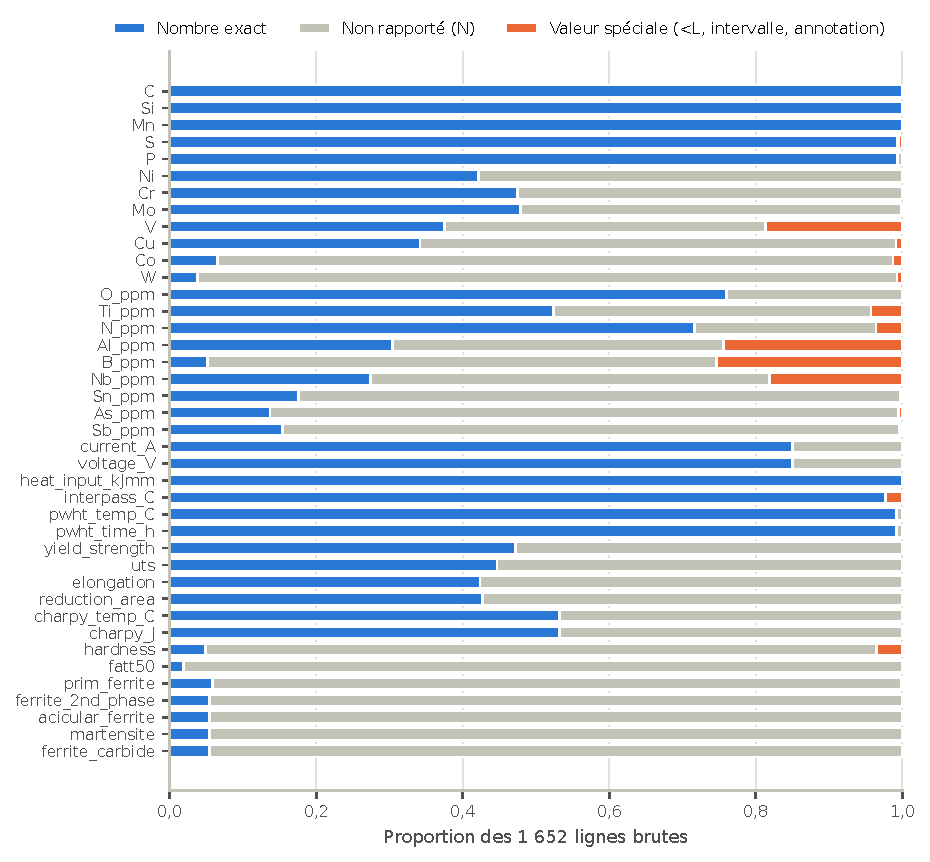
\includegraphics[width=0.93\textwidth]{eda_statuts_mesures}
\caption{Statut des 1\,652 valeurs de chaque variable numérique dans le fichier brut.
Les valeurs spéciales (censures, intervalles, annotations) sont de l'information
rapportée : elles ne doivent être confondues ni avec une absence ni avec un nombre exact.}
\label{fig:statuts}
\end{figure}

La \cref{fig:statuts} montre trois situations très différentes. Le carbone, le
silicium, le manganèse, l'apport thermique et le procédé sont renseignés sur
toutes les lignes. À l'inverse, la microstructure, la dureté et FATT50 sont
presque toujours absentes. Entre les deux, Ni, Cr, Mo, O, N, le courant et la
tension sont partiellement renseignés. \textbf{Aucune ligne n'est complète sur
les 44 colonnes} : supprimer les lignes incomplètes supprimerait toute la base.
Le \cref{tab:speciales} détaille les variables les plus concernées par la
censure ou les annotations.

\begin{table}[htbp]
\centering
\small
\caption{Variables les plus concernées par les valeurs spéciales (fichier brut, 1\,652 lignes).}
\label{tab:speciales}
\begin{tabular}{@{}lrrrr@{}}
\toprule
Variable & Nombres exacts & Censurées & Intervalles/annotations & Non rapportées \\
\midrule
Aluminium                 & 502   & 403 & 0  & 747   \\
Vanadium                  & 620   & 308 & 0  & 724   \\
Bore                      & 85    & 419 & 0  & 1\,148 \\
Niobium                   & 453   & 299 & 0  & 900   \\
Azote                     & 1\,183 & 0  & 59 & 410   \\
Température entre passes  & 1\,614 & 0  & 38 & 0     \\
Dureté                    & 80    & 0   & 58 & 1\,514 \\
FATT50                    & 31    & 0   & 0  & 1\,621 \\
\bottomrule
\end{tabular}
\end{table}

Pour l'aluminium, 44,5\,\% des valeurs rapportées sont censurées ; pour le bore,
83,1\,\%. Un histogramme calculé sur les seuls nombres exacts décrirait donc un
sous-ensemble sélectionné. Les annotations de dureté (\texttt{Hv5}, \texttt{Hv10},
\texttt{Hv30}) renvoient à des protocoles Vickers différents : les nombres
annotés vont de 143 à 467, alors que les valeurs non annotées s'arrêtent à 265.

\subsection{Identifiants, répétitions et séries}
\label{subsec:eda_series}

Les 1\,652 lignes portent \textbf{1\,490 identifiants distincts} ; 91 identifiants
apparaissent plusieurs fois et concernent 253 lignes (par exemple un même dépôt
testé en Charpy à plusieurs températures). Aucune ligne n'est un doublon exact sur
les 44 colonnes, mais \textbf{quatre lignes répètent exactement une autre ligne
lorsqu'on ignore l'identifiant} (indices bruts 393, 423, 425 et 1\,434, qui
dupliquent 333, 363, 365 et 1\,418).

Surtout, les identifiants révèlent des \textbf{séries expérimentales} : par exemple
\ident{Evans-Ni/CMn-1990/1991-0Aaw} et \ident{Evans-Ni/CMn-1990/1991-0Aawch}
appartiennent à la même étude, qui fait varier un seul élément d'alliage à
procédé et protocole constants. Les observations d'une même série partagent la
composition de base, le matériel, les opérateurs et le laboratoire d'essai.

\begin{precaution}
Si l'on mélange aléatoirement les lignes, une soudure de la validation a presque
toujours une \og sœur \fg{} de la même série dans l'entraînement. Le score obtenu
mesure alors la capacité à \emph{interpoler à l'intérieur de séries connues}, et
non à prédire une nouvelle étude. Cette observation motive la validation par
groupes décrite en \cref{sec:protocole}.
\end{precaution}

\subsection{Distributions et ordres de grandeur}

La \cref{fig:distributions} présente les distributions de neuf variables après
retrait des quatre doublons, sur les seuls nombres exacts ; le \cref{tab:ordres}
donne les ordres de grandeur correspondants.

\begin{figure}[htbp]
\centering
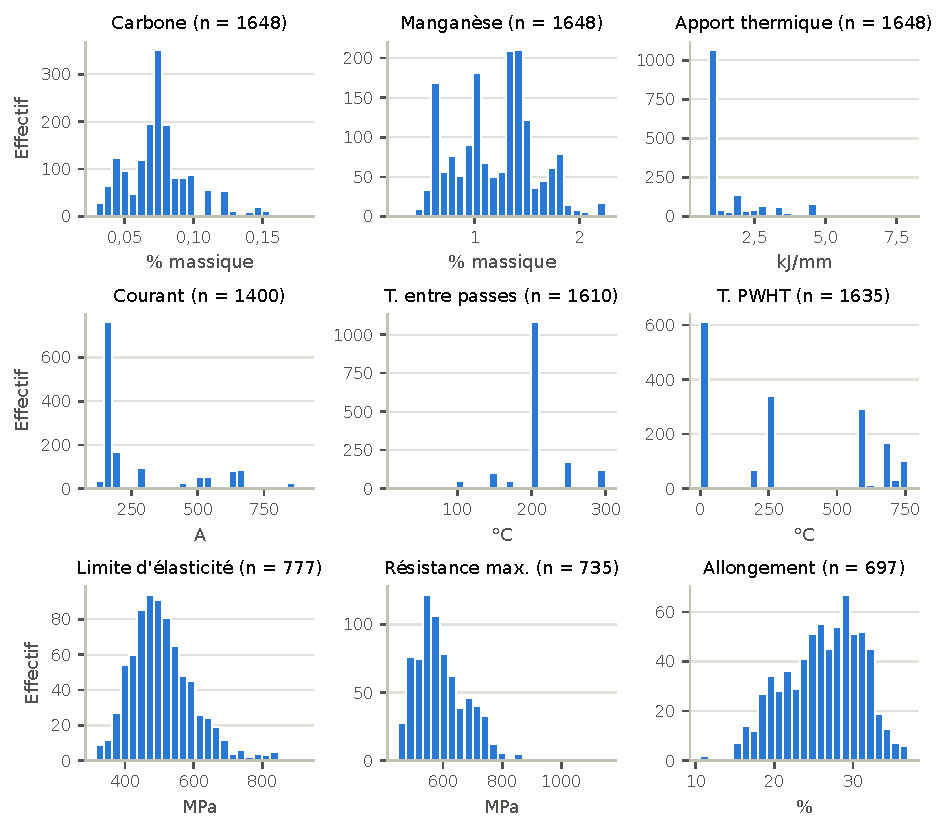
\includegraphics[width=\textwidth]{eda_distributions}
\caption{Distributions de compositions, de paramètres de soudage et de propriétés
mécaniques (nombres exacts, 1\,648 lignes dédupliquées ; $n$ = effectif disponible).
Aucune valeur extrême n'est supprimée et aucune unité n'est convertie.}
\label{fig:distributions}
\end{figure}

\begin{table}[htbp]
\centering
\small
\caption{Ordres de grandeur des principales entrées (nombres exacts, lignes dédupliquées).}
\label{tab:ordres}
\begin{tabular}{@{}llrrrr@{}}
\toprule
Variable & Unité & Effectif & Minimum & Médiane & Maximum \\
\midrule
Carbone                    & \% mass. & 1\,648 & 0,029 & 0,074 & 0,18 \\
Silicium                   & \% mass. & 1\,648 & 0,04  & 0,32  & 1,14 \\
Manganèse                  & \% mass. & 1\,648 & 0,27  & 1,27  & 2,25 \\
Nickel                     & \% mass. & 696   & 0     & 0,0675 & 3,5 \\
Chrome                     & \% mass. & 783   & 0     & 0,53  & 10,2 \\
Molybdène                  & \% mass. & 790   & 0     & 0,34  & 1,5 \\
Oxygène                    & ppm      & 1\,253 & 132  & 423   & 1\,650 \\
Azote (non annoté)         & ppm      & 1\,180 & 21   & 83    & 552 \\
Courant                    & A        & 1\,400 & 115  & 170   & 900 \\
Tension                    & V        & 1\,400 & 11,5 & 21    & 75,36 \\
Apport thermique           & kJ/mm    & 1\,648 & 0,6  & 1     & 7,9 \\
Température entre passes   & °C       & 1\,610 & 20   & 200   & 300 \\
Température PWHT           & °C       & 1\,635 & 0    & 250   & 760 \\
Durée PWHT                 & h        & 1\,635 & 0    & 2     & 24 \\
Température d'essai Charpy & °C       & 877   & $-114$ & $-40$ & 188 \\
\bottomrule
\end{tabular}
\end{table}

Plusieurs observations orientent le prétraitement :
\begin{itemize}
  \item \textbf{Distributions multimodales.} Le manganèse présente plusieurs pics ; le chrome forme des groupes autour de faibles teneurs, de 2\,\% et de 9\,\%. Ces structures traduisent un \emph{mélange de familles d'aciers et de séries expérimentales} plutôt qu'une loi unique.
  \item \textbf{Régimes de procédé.} Les 30 lignes entre 850 et 900\,A appartiennent toutes au procédé sous flux \texttt{SA}, alors que le courant médian est de 170\,A. Ces valeurs sont cohérentes avec le procédé et ne sont pas des anomalies.
  \item \textbf{Réglages répétés.} Les pics d'apport thermique (1\,kJ/mm), de température entre passes (200\,°C) et de PWHT correspondent à des réglages standard répétés.
  \item \textbf{Zéros PWHT.} 610 lignes ont le couple (0\,°C, 0\,h), qui code vraisemblablement un état brut de soudage. Ces zéros mesurés sont conservés tels quels.
  \item \textbf{Valeurs élevées regroupées.} Les plus fortes teneurs en soufre (0,14\,\%) et phosphore (0,25\,\%) apparaissent ensemble dans dix lignes d'une même série (\texttt{Mart-G\ldots}) : cela justifie un examen de provenance, pas une suppression automatique.
  \item \textbf{Cibles.} La limite d'élasticité et la résistance maximale sont unimodales avec une queue vers les fortes valeurs ; l'allongement est concentré entre 25 et 30\,\%.
\end{itemize}

\begin{decision}
Les valeurs extrêmes sont \textbf{conservées} : leur amplitude seule ne démontre
pas une erreur, et elles appartiennent souvent à un procédé ou à une série
identifiable. Supprimer ces points réduirait artificiellement la diversité des
conditions que le modèle doit apprendre.
\end{decision}

\subsection{Les absences dépendent du procédé}
\label{subsec:absences_procede}

Les absences ne sont pas réparties au hasard. La \cref{fig:absences_procede}
croise le taux de valeurs non rapportées avec le procédé de soudage (après
regroupement des seuls synonymes documentés \texttt{ShMA}$\to$\texttt{MMA} et
\texttt{SMA}$\to$\texttt{SA}).

\begin{figure}[htbp]
\centering
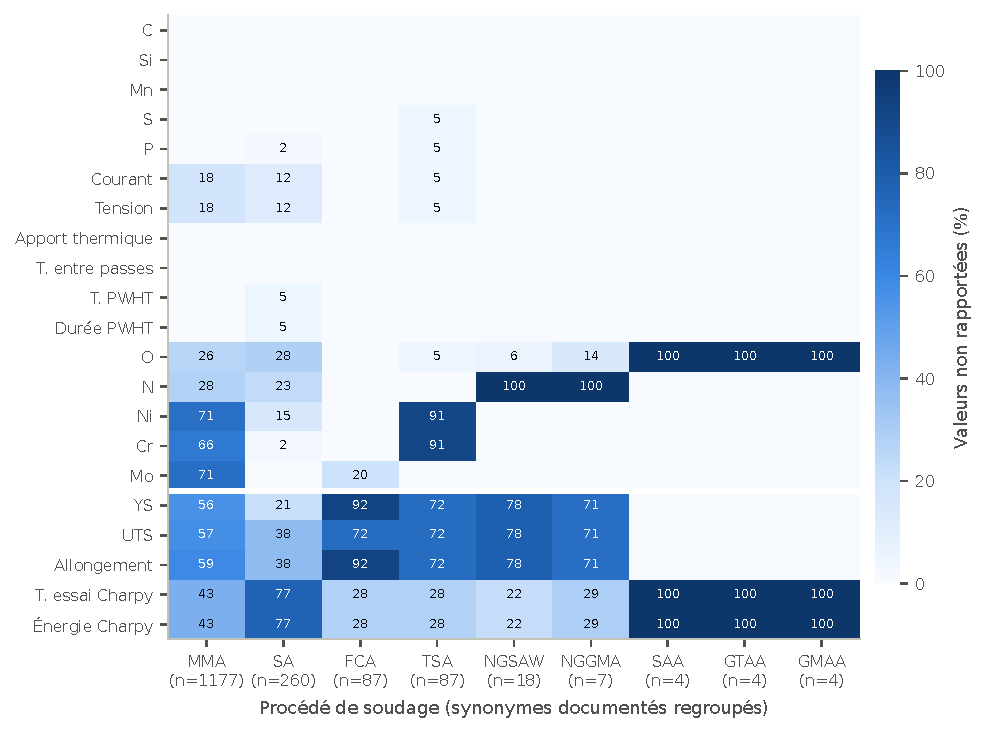
\includegraphics[width=0.95\textwidth]{eda_absences_procede}
\caption{Part de valeurs non rapportées (\%) par procédé, pour les 16 entrées
numériques retenues (haut) et les mesures cibles (bas), sur les 1\,648 lignes
dédupliquées. Cases vides : moins de 0,5\,\% d'absences.}
\label{fig:absences_procede}
\end{figure}

On y lit par exemple que l'oxygène n'est jamais rapporté pour les procédés
\texttt{SAA}, \texttt{GTAA} et \texttt{GMAA}, que l'azote manque toujours pour
\texttt{NGSAW} et \texttt{NGGMA}, que Ni et Cr manquent dans 91\,\% des lignes
\texttt{TSA}, ou que l'énergie Charpy manque dans 77\,\% des lignes \texttt{SA}.
En statistique des données manquantes, ces absences ne sont donc pas
\og complètement aléatoires \fg{} (MCAR)~\cite{little_rubin_2019} : elles dépendent
au moins du procédé et de la source.

\begin{precaution}
Une valeur imputée n'est pas une mesure. Quand l'absence dépend de la source,
l'imputation peut confondre une composition réelle avec la composition
\og typique \fg{} des autres séries. C'est pourquoi l'imputation sera ajustée dans
chaque pli d'entraînement, comparée entre plusieurs méthodes, et ses limites
explicitement testées (\cref{subsec:sensibilites}).
\end{precaution}

\subsection{Cohérence physique et unités douteuses}
\label{subsec:unites}

Les bornes physiques élémentaires sont respectées : concentrations positives,
fractions entre 0 et 100\,\%, températures au-dessus du zéro absolu. Sur les
714 lignes où les deux résistances sont présentes, \textbf{aucune limite
d'élasticité ne dépasse la résistance maximale}. Ce contrôle ne démontre
cependant pas l'homogénéité des unités. Plusieurs indices demandent un retour aux
sources :
\begin{itemize}
  \item \textbf{Aluminium} : dix lignes de la famille \texttt{EPRI-TR-101394s} contiennent 0,004 à 0,014 dans une colonne annoncée en ppm ; en \% massique, cela correspondrait à 40--140\,ppm.
  \item \textbf{Étain, arsenic, antimoine} : les mêmes 90 lignes ont simultanément des valeurs positives inférieures à 1\,ppm, motif typique d'une saisie en \% massique.
  \item \textbf{Titane et vanadium} : une valeur de 0,5\,ppm de titane, des limites \texttt{<0.01} pour Ti/Al (famille \texttt{PantK-1990}) et \texttt{<5} pour V dans une colonne en \% massique.
\end{itemize}
Rappelons que 1\,\% massique $=$ 10\,000\,ppm : multiplier toutes les petites
valeurs par 10\,000 serait une hypothèse non vérifiée. Une normalisation
statistique ne corrigerait pas non plus une erreur d'unité. Ces cellules sont donc
mises en quarantaine (\cref{subsec:nettoyage}). L'audit des publications
(\cref{subsec:charpy_audit}) a d'ailleurs confirmé qu'au moins une source
(Svensson--Gretoft) exprime Ti/Al/Sn/As/Sb en \% massique.

\subsection{Propriétés mesurées et relations entre cibles}
\label{subsec:eda_cibles}

Le \cref{tab:proprietes} recense les propriétés mécaniques candidates. Toutes
sont partiellement renseignées : chaque cible n'est disponible que pour 42 à
53\,\% des lignes.

\begin{table}[htbp]
\centering
\small
\caption{Propriétés mécaniques candidates (nombres exacts du fichier brut).}
\label{tab:proprietes}
\begin{tabular}{@{}lrrrr@{}}
\toprule
Propriété & Mesures & Minimum & Médiane & Maximum \\
\midrule
Limite d'élasticité (MPa)          & 780 & 315  & 495   & 920   \\
Résistance maximale (MPa)          & 738 & 447  & 575,5 & 1\,151 \\
Allongement (\%)                   & 700 & 10,6 & 26,8  & 37    \\
Réduction de section (\%)          & 705 & 17   & 75    & 83    \\
Énergie Charpy (J)                 & 879 & 3    & 100   & 270   \\
Dureté non annotée (kg/mm$^2$)        & 80  & --   & --    & 265   \\
FATT50 (unité non précisée)        & 31  & --   & --    & --    \\
\bottomrule
\end{tabular}
\end{table}

\begin{figure}[htbp]
\centering
\begin{minipage}[c]{0.52\textwidth}
\centering
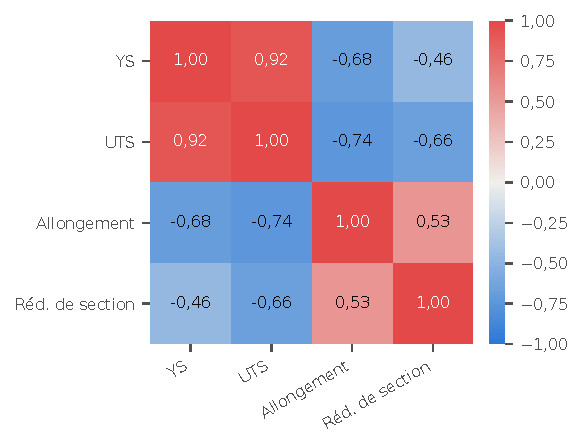
\includegraphics[width=\textwidth]{eda_correlations_cibles}
\end{minipage}\hfill
\begin{minipage}[c]{0.45\textwidth}
\caption{Corrélations de Pearson entre propriétés de traction, calculées sur les
paires observées (lignes dédupliquées). Bleu : corrélation négative ; rouge :
positive. Cette matrice décrit des dépendances par paires ; ce n'est pas une ACP.}
\label{fig:correlations}
\end{minipage}
\end{figure}

La \cref{fig:correlations} montre que \YS{} et \UTS{} sont très corrélées
($r = 0{,}915$), tandis que l'allongement leur est opposé ($r = -0{,}680$ avec
\YS, $-0{,}738$ avec \UTS) : un métal plus résistant est en moyenne moins ductile.
Ces corrélations n'autorisent pas à remplacer une cible par une autre : 0,915
laisse une part substantielle de variation propre à chacune, et résistance et
ductilité sont des informations complémentaires.

L'énergie Charpy doit toujours être lue avec sa température d'essai
(\cref{fig:charpy}). Sur 877 couples exacts dédupliqués, \textbf{355 énergies
valent exactement 100\,J et 118 valent 28\,J}. Ces valeurs correspondent à des
critères classiques de transition ductile-fragile : certaines publications
rapportent la \emph{température} à laquelle l'énergie atteint 100\,J ou 28\,J,
plutôt qu'une énergie mesurée à une température choisie~\cite{evans_1989_cr}.
Les deux protocoles produisent des points d'apparence identique dans la base.

\begin{figure}[htbp]
\centering
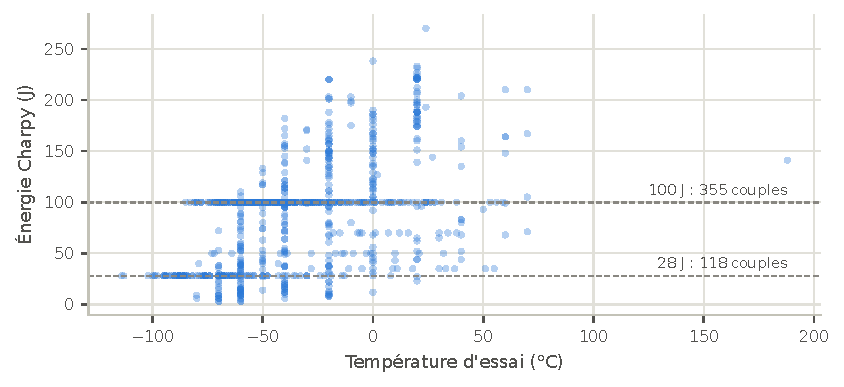
\includegraphics[width=\textwidth]{eda_charpy_couples}
\caption{Couples (température d'essai, énergie Charpy) exacts. Les lignes
horizontales à 28\,J et 100\,J concentrent 54\,\% des points, signature probable
de températures de transition plutôt que de mesures à température imposée.}
\label{fig:charpy}
\end{figure}

\subsection{Analyse en composantes principales descriptive}
\label{subsec:acp}

L'énoncé demande d'appliquer une ACP pour développer une intuition sur le
problème. L'ACP cherche les directions orthogonales de l'espace des entrées qui
expliquent le plus de variance~\cite{jolliffe_2016}. Comme les unités sont
différentes, chaque variable est d'abord \textbf{standardisée} (moyenne nulle,
écart-type unité) ; sinon le courant (centaines d'ampères) écraserait le carbone
(centièmes de pourcent).

\begin{decision}
L'ACP porte sur les \textbf{1\,339 lignes dédupliquées dont les onze entrées de
base sont des nombres exacts complets} (C, Si, Mn, S, P, courant, tension, apport
thermique, température entre passes, température et durée PWHT), \textbf{sans
imputation}. Ainsi, la structure observée n'est pas fabriquée par des valeurs
reconstruites. En contrepartie, cette sous-population peut différer de la base
entière, et l'ACP reste descriptive : elle n'est réutilisée ni pour entraîner ni
pour évaluer les modèles.
\end{decision}

\begin{figure}[htbp]
\centering
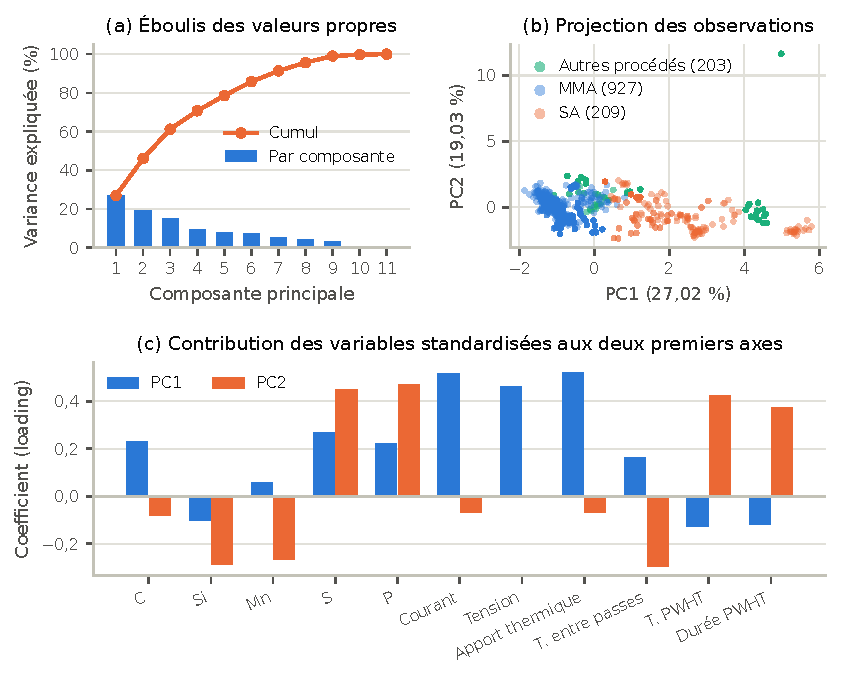
\includegraphics[width=\textwidth]{eda_acp}
\caption{ACP standardisée des onze entrées complètes (1\,339 lignes). (a) Variance
expliquée par composante et cumul. (b) Projection sur les deux premiers axes,
colorée par procédé. (c) Coefficients des variables sur les deux premiers axes.}
\label{fig:acp}
\end{figure}

Les deux premiers axes expliquent \textbf{27,02\,\%} et \textbf{19,03\,\%} de la
variance, soit 46,05\,\% cumulés ; trois axes en expliquent 61,26\,\% et il faut
huit axes pour dépasser 95\,\% (\cref{fig:acp}a). L'information est donc
\emph{répartie} sur de nombreuses directions. L'interprétation des axes
(\cref{fig:acp}c) est néanmoins éclairante :
\begin{itemize}
  \item \textbf{PC1 --- \og énergie du procédé \fg{}.} Les coefficients les plus forts sont l'apport thermique (0,52), le courant (0,52) et la tension (0,46). Cet axe sépare nettement le soudage manuel \texttt{MMA}, à faible courant, du soudage sous flux \texttt{SA}, à fort courant (\cref{fig:acp}b).
  \item \textbf{PC2 --- \og impuretés et traitement thermique \fg{}.} Le phosphore (0,47), le soufre (0,45), la température (0,43) et la durée (0,37) du PWHT s'opposent au silicium ($-0{,}29$), à la température entre passes ($-0{,}29$) et au manganèse ($-0{,}27$).
\end{itemize}
La projection montre des amas compacts correspondant à des séries et des procédés,
plutôt qu'un nuage continu. L'ACP confirme ainsi, du point de vue des entrées,
la structure en séries identifiée par les identifiants.

\begin{decision}
Aucune ACP n'est incluse dans les pipelines prédictives : les deux premiers axes
ne résument que 46\,\% de la variance, les forêts aléatoires n'en ont pas besoin,
et une réduction de dimension aurait dû être réapprise dans chaque pli. Une ACP
ajustée sur toute la base puis réutilisée en validation constituerait une fuite
d'information.
\end{decision}

\subsection{Bilan de l'analyse exploratoire}

\begin{aretenir}
\begin{itemize}[leftmargin=1.2em]
  \item La base est une \textbf{compilation de séries expérimentales} : observations apparentées, compositions multimodales, procédés déséquilibrés (\texttt{MMA} majoritaire).
  \item \texttt{N} signifie \textbf{non rapporté} ; censures, intervalles et annotations sont des informations à conserver, pas à confondre avec des nombres exacts.
  \item Les absences \textbf{dépendent du procédé et de la source} ; aucune ligne n'est complète.
  \item Quelques cellules ont une \textbf{unité douteuse} ; elles doivent être isolées sans conversion conjecturale.
  \item Les cibles sont partiellement renseignées et corrélées sans être interchangeables ; l'énergie Charpy mélange probablement plusieurs protocoles.
  \item L'ACP met en évidence un axe \og énergie du procédé \fg{} et un axe \og impuretés/PWHT \fg{}, et confirme une structure en amas liée aux séries.
\end{itemize}
\end{aretenir}

% =====================================================================
%  3. Variables cibles et stratégie de prédiction
% =====================================================================
\clearpage
\section{Variables cibles et stratégie de prédiction}
\label{sec:cibles}

\subsection{Quelles variables représentent la qualité ?}

À partir de l'EDA, nous retenons comme \textbf{cibles principales} les trois
propriétés de traction --- \YS, \UTS{} et allongement --- et comme \textbf{cible
exploratoire} l'énergie Charpy à température d'essai connue. Le
\cref{tab:cibles} justifie ce choix et donne les effectifs à chaque étape du
filtrage décrit en \cref{sec:prep}.

\begin{table}[htbp]
\centering
\small
\caption{Cibles retenues et effectifs de labels. \og Cohorte \fg{} désigne la
population de modélisation de 1\,555 lignes (\cref{subsec:cohorte}) ;
\og Groupes \fg{} le nombre de séries inférées portant au moins un label.}
\label{tab:cibles}
\begin{tabularx}{\textwidth}{@{}l l r r r r L@{}}
\toprule
Cible & Unité & Brut & Dédupl. & Cohorte & Groupes & Rôle et justification \\
\midrule
\YS           & MPa & 780 & 777 & 706 & 40 & Principale : propriété de dimensionnement, bonne couverture \\
\UTS          & MPa & 738 & 735 & 677 & 39 & Principale : résistance, complémentaire de \YS \\
Allongement   & \%  & 700 & 697 & 631 & 34 & Principale : ductilité, opposée à la résistance \\
Énergie \charpy & J & 879 & 877 & 861 & 24 & Exploratoire : protocoles hétérogènes (\cref{subsec:charpy_strategie}) \\
\midrule
Réduction de section & \% & 705 & 702 & 635 & -- & Complémentaire, non entraînée \\
Dureté        & kg/mm$^2$ & 138 & -- & -- & -- & Écartée : 80 valeurs exactes, protocoles Vickers mélangés \\
FATT50        & ?   & 31  & -- & -- & -- & Écartée : 31 valeurs, unité non documentée \\
\bottomrule
\end{tabularx}
\end{table}

Les distributions des cibles dans la cohorte sont résumées au \cref{tab:stats_cibles}.

\begin{table}[htbp]
\centering
\small
\caption{Statistiques des cibles dans la cohorte de modélisation.}
\label{tab:stats_cibles}
\begin{tabular}{@{}lrrrr@{}}
\toprule
Cible & Labels & Médiane & Minimum & Maximum \\
\midrule
\YS{} (MPa)              & 706 & 496,0 & 315,0 & 920,0 \\
\UTS{} (MPa)             & 677 & 576,0 & 447,0 & 1\,151,0 \\
Allongement (\%)         & 631 & 26,6  & 10,6  & 36,4 \\
Énergie \charpy{} (J)    & 861 & 100,0 & 3,0   & 270,0 \\
\bottomrule
\end{tabular}
\end{table}

\subsection{Pourquoi des régressions séparées ?}

Dans la cohorte, seules \textbf{609 lignes} renseignent simultanément les trois
propriétés de traction et \textbf{141} les quatre cibles. Un modèle
multi-sorties exigeant les trois propriétés de traction perdrait 14\,\% des
labels de \YS ; exiger les quatre cibles ne conserverait que 16 à 22\,\% des
labels selon la cible. Il faudrait sinon imputer des cibles, ce qui reviendrait
à entraîner sur des valeurs inventées.

\begin{decision}
Chaque cible dispose de \textbf{son propre modèle et de ses propres lignes
d'entraînement} : on apprend la cible $t$ sur toutes les lignes qui renseignent
$t$, sans exiger les autres. Une cible absente reste inconnue et
\textbf{n'est jamais imputée}. Aucune propriété mécanique n'est utilisée comme
entrée pour en prédire une autre, car elle ne serait pas disponible au moment
d'estimer une soudure non encore testée.
\end{decision}

\subsection{Le cas particulier de l'énergie Charpy}
\label{subsec:charpy_strategie}

Deux formulations sont possibles pour la ténacité : prédire l'énergie $E$ à une
température $T$ donnée, ou prédire la température $T_{100\,\mathrm{J}}$ (ou
$T_{28\,\mathrm{J}}$) à laquelle l'énergie atteint un seuil. Nous retenons la
première, \textbf{$E(T)$ avec la température d'essai en entrée}, formulation
utilisée par des travaux de référence sur cette famille de données~\cite{bhadeshia_1995,cool_1996}.
La température n'est jamais reconstruite : seules les 861 lignes de la cohorte
où elle est connue sont utilisées.

\begin{precaution}
La documentation définit bien deux colonnes distinctes (température en °C,
énergie en J), mais pas le protocole de chaque ligne. Une partie des couples
correspond probablement à des températures de transition à 28 ou 100\,J
(\cref{fig:charpy}), une autre à des courbes $E(T)$ complètes. Aucun seuil
28/100\,J ne sert à exclure automatiquement des lignes : cette tâche est traitée
comme \textbf{exploratoire} et les sources ont été auditées a posteriori
(\cref{subsec:charpy_audit}).
\end{precaution}

\subsection{Entrées autorisées et entrées exclues}
\label{subsec:entrees_exclues}

Une variable n'est utilisée en entrée que si elle serait connue \emph{avant}
l'essai mécanique, dans un usage réaliste du modèle. Le \cref{tab:entrees_exclues}
résume cette règle.

\begin{table}[htbp]
\centering
\small
\caption{Entrées autorisées et exclues des modèles.}
\label{tab:entrees_exclues}
\begin{tabularx}{\textwidth}{@{}l L@{}}
\toprule
Statut & Variables et raison \\
\midrule
\textbf{Autorisées} & Composition (C, Si, Mn, S, P, Ni, Cr, Mo, O, N), courant, tension, apport thermique, température entre passes, température et durée PWHT, procédé ; pour Charpy uniquement : température d'essai. \\
\addlinespace
Exclues (fuite) & Autres propriétés mécaniques, dureté, FATT50 : mesurées après l'essai, indisponibles pour une soudure nouvelle. \\
Exclues (fuite) & Identifiant, série, groupe, numéro de pli, drapeaux d'éligibilité : ils renseigneraient sur la source et non sur la soudure. \\
Exclues (disponibilité) & Microstructure : observée après soudage, 89 à 98 valeurs par colonne seulement. \\
Exclues (fiabilité) & V, Cu, Co, W, Ti, Al, B, Nb, Sn, As, Sb : couverture faible, censures nombreuses ou unités douteuses. Cette exclusion ne signifie pas que ces éléments n'ont pas d'effet métallurgique. \\
Non utilisées & Type de courant et polarité : conservés dans la table maître (modalité \texttt{missing} si non rapportés), non retenus dans les schémas d'entrées. \\
\bottomrule
\end{tabularx}
\end{table}

\subsection{Stratégie d'ensemble}

La stratégie de prédiction se déroule en cinq temps :
\begin{enumerate}
  \item \textbf{Construire une population fiable} : nettoyage déterministe, déduplication, groupes de séries et cohorte avec peu d'entrées manquantes (\cref{sec:prep}).
  \item \textbf{Fixer une référence minimale} : prédire la médiane de $y$ du train, sans utiliser $\bm{x}$. Tout modèle doit faire mieux.
  \item \textbf{Comparer des familles de modèles vues en cours}, du linéaire régularisé (Ridge) aux méthodes non linéaires (SVR, forêt aléatoire, $k$NN), avec réglage des hyperparamètres par validation croisée \textbf{imbriquée} (\cref{sec:methodes,sec:protocole}).
  \item \textbf{Évaluer selon deux usages} : interpolation dans des séries connues (découpage aléatoire) et transfert à de nouvelles séries (découpage groupé).
  \item \textbf{Exploiter les lignes non étiquetées} avec une méthode semi-supervisée (COREG), comparée à son exact pendant supervisé.
\end{enumerate}

Les lignes de la cohorte sans la cible forment le \textbf{pool non étiqueté} de
cette cible : 849 lignes pour \YS, 878 pour \UTS{} et 924 pour l'allongement.
Pour Charpy, \textbf{aucune} ligne de la cohorte n'a une température d'essai
connue sans énergie : le pool naturel est vide, et aucune température n'est
fabriquée pour en créer un.

\begin{aretenir}
Quatre régressions indépendantes : \YS, \UTS, allongement (principales) et
énergie Charpy $E(T)$ (exploratoire). Les entrées sont limitées à ce qui est
connu avant l'essai ; aucune cible n'est imputée ni utilisée comme entrée. Les
lignes sans cible alimentent l'étude semi-supervisée pour les trois cibles de
traction.
\end{aretenir}

% =====================================================================
%  4. Préparation des données
% =====================================================================
\clearpage
\section{Préparation des données}
\label{sec:prep}

La préparation (notebook \notebook{02\_data\_preparation.ipynb}) transforme le
fichier brut en une table maître traçable, définit les groupes, la cohorte et
les plis, puis fournit le prétraitement qui sera appris \emph{à l'intérieur} de
chaque entraînement. Elle a d'abord été prototypée, auditée à deux reprises
(rapports 06 et 07 du dépôt), puis migrée dans ce notebook autonome ; les huit
exports migrés reproduisent exactement les exports audités.

\subsection{Deux niveaux de traitement}

Il est essentiel de distinguer deux types d'opérations :
\begin{description}[leftmargin=1em,style=nextline]
  \item[Nettoyage déterministe (global)] règles fixées \emph{a priori}, qui ne
  dépendent d'aucune statistique apprise : interpréter \texttt{N}, remplacer une
  censure par une valeur conventionnelle, isoler une unité douteuse. Elles
  peuvent être appliquées à toute la base sans fuite d'information.
  \item[Prétraitement appris (dans les plis)] opérations qui estiment des
  paramètres sur les données : moyennes et écarts-types, médianes, catégories
  connues, modèles d'imputation. Elles sont \textbf{réajustées sur chaque ensemble
  d'entraînement}, puis appliquées telles quelles à la validation correspondante.
\end{description}

\begin{intuition}
Si l'on calculait la médiane d'imputation ou la moyenne de standardisation sur
toute la base, la validation \og verrait \fg{} indirectement ses propres valeurs
à travers ces statistiques : le score serait légèrement optimiste. Ajuster ces
statistiques dans le train seulement reproduit la situation réelle, où une
nouvelle soudure arrive après l'entraînement.
\end{intuition}

\subsection{Nettoyage déterministe}
\label{subsec:nettoyage}

Le \cref{tab:nettoyage} récapitule chaque règle et sa justification. Le résultat
est une \textbf{table maître de 1\,652 lignes} (dont quatre alias marqués) et un
fichier de \textbf{provenance de 66\,080 cellules numériques} (1\,652 lignes
$\times$ 40 colonnes numériques) qui conserve, pour chaque cellule, le jeton
brut, son statut, ses bornes, l'opérateur de censure, l'annotation éventuelle,
le drapeau de revue et la valeur retenue. Aucune cible observée n'est modifiée.

\begin{table}[htbp]
\centering
\small
\caption{Règles de nettoyage déterministe et justification.}
\label{tab:nettoyage}
\begin{tabularx}{\textwidth}{@{}>{\raggedright\arraybackslash}p{3.6cm} >{\raggedright\arraybackslash}p{4.6cm} L@{}}
\toprule
Situation & Règle appliquée & Justification \\
\midrule
Lecture & 44 champs lus comme texte ; identifiant brut \texttt{raw\_row\_id} stable (0 à 1\,651) & Ne rien perdre avant d'avoir classé chaque jeton \\
\texttt{N} (non rapporté) & Valeur manquante (NaN), jamais zéro & Définition de la documentation source \\
Nombres exacts, zéros, extrêmes & Conservés & Une valeur extrême n'est pas une erreur démontrée \\
Censure \texttt{<L} sans doute d'unité & $L/2$, avec statut, opérateur et borne conservés & Approximation conventionnelle, explicitement signalée comme telle \\
Intervalle \texttt{a-b} & Milieu $(a+b)/2$, bornes conservées & 38 températures entre passes \texttt{150-200} $\to$ 175\,°C \\
Unité douteuse & NaN, sans conversion ; 322 cellules : Al 26, Ti 17, V 9, Sn/As/Sb 90 chacun & Seule la source peut confirmer l'unité (\cref{subsec:unites}) \\
Azote annoté (\texttt{tot}/\texttt{res}) & 59 annotations hors de N principal, extraction lexicale conservée & Sens total/résiduel non comparable aux autres valeurs \\
Dureté & Valeur et protocole Vickers séparés & Protocoles non regroupés automatiquement \\
Procédé & Seuls \texttt{ShMA}$\to$\texttt{MMA} et \texttt{SMA}$\to$\texttt{SA} & Synonymes documentés ; les autres procédés restent distincts \\
Courant et polarité & \texttt{N} $\to$ modalité \texttt{missing} ; aucune déduction DC/AC & Ne pas inventer une catégorie \\
Doublons hors identifiant & 4 occurrences excédentaires exclues de la cohorte et des plis ; alias conservés & Éviter qu'une même observation soit en train et en validation \\
PWHT & 13 lignes PWHT manquant conservées ; couples (0, 0) conservés & Le sens métallurgique exact du zéro n'est pas affirmé \\
\bottomrule
\end{tabularx}
\end{table}

\begin{precaution}
Les choix $L/2$ et milieu d'intervalle sont des \emph{approximations
déterministes}, pas des mesures. Ils concernent surtout des éléments absents des
schémas d'entrées retenus (Al, B, Nb, V). Pour les 16 entrées retenues, seules
47 cellules du fichier brut sont concernées : 38 intervalles de température entre passes, 7
censures de soufre et 2 de molybdène (les 59 azotes annotés étant indisponibles).
Le statut d'origine reste disponible pour toute analyse de sensibilité.
\end{precaution}

\subsection{Groupes : des séries expérimentales inférées}
\label{subsec:groupes}

Pour évaluer le transfert à de nouvelles séries, il faut d'abord les définir.
La base ne fournit pas de numéro de publication ; les groupes sont donc
\textbf{inférés des identifiants}, de manière conservatrice :
\begin{enumerate}
  \item préfixe de l'identifiant jusqu'à l'année (\ident{Evans-Ni/CMn-1990/1991-0Aaw} $\to$ \ident{Evans-Ni/CMn-1990}) ;
  \item familles explicites de rapports ou de lettres (par exemple \texttt{EvansLetter}) ;
  \item préfixe non daté, ou identifiant exact en dernier recours ;
  \item les doublons bruts relient leurs séries respectives.
\end{enumerate}
On obtient \textbf{47 groupes} sur les 1\,648 lignes dédupliquées. Les variantes
orthographiques d'auteurs (\texttt{Ga\&K}/\texttt{Gar\&K}, \texttt{Kocak}) ne sont
pas fusionnées dans le protocole actif. Ces groupes sont des \emph{séries
inférées}, pas des publications vérifiées : une série peut regrouper plusieurs
conditions de soudage (\cref{subsec:decoupages}).

\subsection{Cohorte de modélisation}
\label{subsec:cohorte}

Ni, Cr et Mo sont absents dans plus de la moitié des lignes ; d'autres entrées
le sont plus rarement. Nous définissons une cohorte qui limite le nombre
d'entrées à reconstruire tout en conservant un maximum de séries :

\begin{decision}
\textbf{Cohorte principale} : lignes non dupliquées ayant \textbf{au plus deux
entrées numériques indisponibles parmi les 13 entrées du schéma A1\_13}
(\cref{tab:schemas}). Elle compte \textbf{1\,555 lignes réparties en 44 groupes} ;
trois séries (\texttt{Cunh-1982}, \texttt{EvHtIp1979}, \texttt{Natsume-1990})
sortent entièrement. Les seuils alternatifs $\leq 1$ et $\leq 3$ donneraient
1\,087 et 1\,603 lignes, 34 et 46 groupes, 501 et 748 labels de \YS{} : le
seuil 2 est un compromis d'ingénierie entre couverture et quantité d'imputation,
pas une garantie de fiabilité.
\end{decision}

\begin{figure}[htbp]
\centering
\begin{tikzpicture}[
  bloc/.style={rectangle, rounded corners=2pt, draw=csbordeaux, line width=0.7pt,
               fill=csgrisclair, align=center, minimum height=1.05cm, font=\footnotesize},
  cible/.style={rectangle, rounded corners=2pt, draw=csgris, line width=0.6pt,
               fill=white, align=center, minimum height=0.95cm, text width=2.55cm, font=\scriptsize},
  fleche/.style={-{Stealth[length=2mm]}, line width=0.8pt, color=csgris},
  lab/.style={font=\scriptsize\itshape, color=encre2, align=left}]
  \node[bloc, text width=3.1cm] (brut) {\textbf{1\,652 lignes brutes}\\ 44 colonnes};
  \node[bloc, text width=3.1cm, right=1.9cm of brut] (dedup) {\textbf{1\,648 lignes}\\ dédupliquées, 47 groupes};
  \node[bloc, text width=3.4cm, right=1.9cm of dedup] (coh) {\textbf{1\,555 lignes, 44 groupes}\\ cohorte $\leq 2$ absences sur A1\_13};
  \draw[fleche] (brut) -- node[above, lab] {$-4$ alias} (dedup);
  \draw[fleche] (dedup) -- node[above, lab] {$-93$ lignes} (coh);
  \node[cible, below=1.25cm of brut.south west, anchor=north west] (ys) {\textbf{\YS} : 706 labels\\ 40 groupes ; pool 849};
  \node[cible, right=0.35cm of ys] (uts) {\textbf{\UTS} : 677 labels\\ 39 groupes ; pool 878};
  \node[cible, right=0.35cm of uts] (el) {\textbf{Allongement} : 631\\ 34 groupes ; pool 924};
  \node[cible, right=0.35cm of el] (ch) {\textbf{\charpy} : 861\\ 24 groupes ; pool 0};
  \draw[fleche] (coh.south) -- ++(0,-0.45) -| (ys.north);
  \draw[fleche] (coh.south) -- ++(0,-0.45) -| (uts.north);
  \draw[fleche] (coh.south) -- ++(0,-0.45) -| (el.north);
  \draw[fleche] (coh.south) -- ++(0,-0.45) -| (ch.north);
\end{tikzpicture}
\caption{Du fichier brut aux populations de modélisation. Chaque cible utilise les
lignes de la cohorte qui la renseignent ; les autres lignes de la cohorte forment
son pool non étiqueté (vide pour Charpy, faute de température d'essai connue sans énergie).}
\label{fig:entonnoir}
\end{figure}

Dans la cohorte, \textbf{607 lignes} ont au moins une entrée absente parmi les
13, soit \textbf{1\,075 cellules}. La table maître conserve ces NaN : aucune
table globalement imputée n'est utilisée par les modèles. Parmi les lignes
dédupliquées, 105 n'ont aucune des cinq sorties traction/Charpy (99 dans la
cohorte) ; elles sont conservées comme exemples non étiquetés.

\subsection{Schémas d'entrées}
\label{subsec:schemas}

Trois schémas emboîtés ont été définis et comparés (\cref{tab:schemas}). Le
schéma de départ A1\_13 privilégiait des entrées bien renseignées ; l'extension
A1b\_16 ajoute Ni, Cr et Mo, éléments d'alliage métallurgiquement importants
mais souvent absents (\cref{fig:absences_cohorte}). Passer de 13 à 16 entrées
\textbf{ajoute des colonnes, pas des lignes} : la cohorte n'est pas refiltrée.

\begin{table}[htbp]
\centering
\small
\caption{Schémas d'entrées numériques ; le procédé catégoriel est ajouté à chacun.}
\label{tab:schemas}
\begin{tabularx}{\textwidth}{@{}l c L@{}}
\toprule
Schéma & Entrées & Variables \\
\midrule
A0\_11  & 11 & C, Si, Mn, S, P, courant, tension, apport thermique, température entre passes, température et durée PWHT \\
A1\_13  & 13 & A0\_11 $+$ oxygène et azote \\
A1b\_16 & 16 & A1\_13 $+$ nickel, chrome et molybdène \\
\bottomrule
\end{tabularx}
\end{table}

\begin{figure}[htbp]
\centering
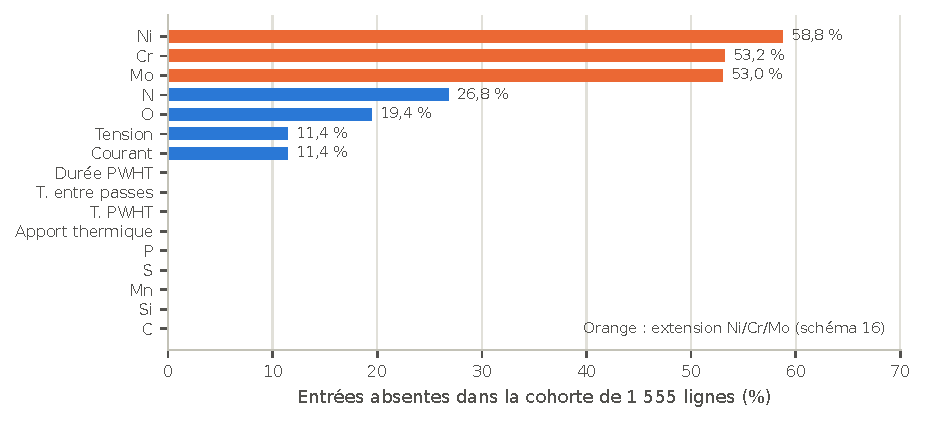
\includegraphics[width=0.95\textwidth]{prep_absences_cohorte}
\caption{Part d'entrées absentes dans la cohorte de 1\,555 lignes pour les
16 entrées numériques. Ni, Cr et Mo manquent dans plus de la moitié des lignes.}
\label{fig:absences_cohorte}
\end{figure}

\subsection{Normalisation : pourquoi standardiser ?}
\label{subsec:standardisation}

Chaque entrée numérique est standardisée avec la moyenne $\mu_j$ et
l'écart-type $\sigma_j$ calculés sur les valeurs \emph{observées} du train :
\begin{equation}
  z_{ij} = \frac{x_{ij} - \mu_j^{\text{train}}}{\sigma_j^{\text{train}}}.
\end{equation}
Cette étape est indispensable pour les méthodes fondées sur des distances ou des
normes : le $k$NN, la SVR à noyau RBF (dont le noyau
$\exp(-\gamma\lVert\bm{x}-\bm{x}'\rVert^2)$ dépend des échelles) et la régression
Ridge (dont la pénalité $\lambda\lVert\bm{\beta}\rVert^2$ traite tous les
coefficients de la même manière). Elle est sans effet sur les partitions d'une
forêt aléatoire, mais elle est conservée pour que toutes les familles partagent
exactement la même représentation. Le procédé est encodé en \emph{one-hot} sur
les catégories vues dans le train ; une catégorie inconnue devient un vecteur nul.
Pour la SVR uniquement, la cible $y$ est aussi standardisée dans le train, puis
les prédictions sont remises dans leur unité physique.

\subsection{Imputation des entrées manquantes}
\label{subsec:imputation}

Deux méthodes d'imputation ont été mises en œuvre, toutes deux \textbf{ajustées
dans chaque train} et appliquées aux seules \emph{entrées} :
\begin{description}[leftmargin=1em,style=nextline]
  \item[Médiane] chaque valeur manquante reçoit la médiane de la colonne dans le
  train. Simple et stable, elle ignore les relations entre variables.
  \item[Itérative] (\emph{chained equations})~\cite{vanbuuren_2011} chaque
  colonne incomplète est régressée sur les autres par une régression bayésienne
  ridge (\texttt{IterativeImputer} + \texttt{BayesianRidge}), en alternant
  jusqu'à convergence : initialisation médiane, ordre ascendant, au plus 100
  itérations, tolérance $10^{-3}$, graine 42, bornes non négatives.
\end{description}
Après imputation, un PWHT reconstruit est projeté sur un couple
(température, durée) \emph{réellement observé} dans le train, au plus proche en
distance standardisée et compatible avec une composante observée. Toute situation
anormale --- colonne entièrement absente du train, absence de couple compatible,
non-convergence de l'imputation itérative --- déclenche une \textbf{erreur
explicite}, sans repli silencieux. Les cibles ne sont jamais transmises à
l'imputeur.

\paragraph{Pourquoi l'itérative au départ ?} Une étude historique de
reconstruction (5 octobre) masquait artificiellement 10, 20 ou 40\,\% de valeurs
exactes et comparait les méthodes sur des plis par séries (\cref{tab:reconstruction}).
Sur 11 entrées, l'itérative reconstruisait le mieux ; sur une extension à
22 entrées, elle ne convergeait dans aucun pli.

\begin{table}[htbp]
\centering
\small
\caption{Étude historique de reconstruction de valeurs masquées (3 plis par
séries, graines 42/43). MAE normalisée par l'écart interquartile du train ; plus
bas est meilleur.}
\label{tab:reconstruction}
\begin{tabular}{@{}llrrr@{}}
\toprule
Entrées & Méthode & MAE normalisée & $\Delta$ corrélations & Plis convergés \\
\midrule
11 (noyau)    & Médiane              & 1,697 & 0,084 & 3/3 \\
11 (noyau)    & Médiane par procédé  & 1,254 & 0,069 & 3/3 \\
11 (noyau)    & Itérative            & \meilleur{0,853} & \meilleur{0,066} & 3/3 \\
22 (étendu)   & Médiane              & 2,253 & 0,106 & 3/3 \\
22 (étendu)   & Médiane par procédé  & 2,060 & 0,106 & 3/3 \\
22 (étendu)   & Itérative            & 2,009 & 0,159 & 0/3 \\
\bottomrule
\end{tabular}
\end{table}

Un contrôle à paramètres fixes, sur le schéma A1\_13 et les plis groupés, a
ensuite comparé les deux imputations sous une forêt aléatoire (300 arbres,
feuille minimale 2, graine 42). Les 15 ajustements itératifs convergeaient en
4 à 7 itérations, et l'itérative n'était pas uniformément meilleure
(\cref{tab:controle_imputation}).

\begin{table}[htbp]
\centering
\small
\caption{Contrôle d'imputation à paramètres fixes, schéma 13, validation groupée
(MAE moyenne des cinq plis externes).}
\label{tab:controle_imputation}
\begin{tabular}{@{}lrrrr@{}}
\toprule
Cible & Baseline médiane & RF / médiane & RF / itérative & \Rdeux{} RF / itérative \\
\midrule
\YS{} (MPa)               & 70,45 & \meilleur{65,39} & 66,13 & 0,077 \\
\UTS{} (MPa)              & 72,66 & 58,10 & \meilleur{56,71} & 0,190 \\
Allongement (points de \%) & 4,09 & 3,70 & \meilleur{3,55} & 0,114 \\
\bottomrule
\end{tabular}
\end{table}

\begin{decision}
Le premier benchmark supervisé utilise \textbf{A1\_13 avec imputation
itérative}, justifiée par l'étude de reconstruction. Les diagnostics
(\cref{subsec:sensibilites}) montreront ensuite que l'itérative \textbf{ne converge
pas} dans 11 contextes sur 16 entrées, alors que la médiane reste stable et que
l'ajout de Ni/Cr/Mo améliore nettement \YS{} et \UTS. La configuration de travail
devient alors \textbf{A1b\_16 avec imputation médiane}. Ce choix est
rétrospectif : il a été fait après observation des scores sur ces mêmes données.
\end{decision}

\subsection{Le prétraitement complet dans une pipeline}

Toutes les étapes apprises sont encapsulées dans une \texttt{Pipeline} de
scikit-learn~\cite{pedregosa_2011} : la classe \texttt{FoldPreprocessor}, définie
dans le notebook 02, est suivie de l'estimateur. La \cref{fig:pipeline} illustre son
fonctionnement : la même pipeline est ajustée sur le train, puis appliquée
sans réajustement à la validation et, pour COREG, au pool non étiqueté.

\begin{figure}[htbp]
\centering
\begin{tikzpicture}[
  etape/.style={rectangle, rounded corners=2pt, draw=csbordeaux, line width=0.6pt,
                fill=csgrisclair, align=center, text width=2.05cm, minimum height=1.15cm,
                font=\scriptsize},
  data/.style={rectangle, draw=csgris, line width=0.6pt, fill=white, align=center,
               text width=1.8cm, minimum height=0.85cm, font=\scriptsize},
  fit_/.style={-{Stealth[length=1.8mm]}, line width=0.75pt, color=csbordeaux},
  app/.style={-{Stealth[length=1.8mm]}, line width=0.75pt, color=bleuviz, dashed},
  node distance=0.32cm]
  \node[data] (xtr) {Train\\ $(X, y)$ étiqueté};
  \node[etape, right=0.45cm of xtr] (s1) {Moyenne/écart-type\\ des valeurs observées};
  \node[etape, right=of s1] (s2) {One-hot du procédé\\ (catégories du train)};
  \node[etape, right=of s2] (s3) {Imputation\\ médiane ou itérative};
  \node[etape, right=of s3] (s4) {Garde PWHT\\ (couples du train)};
  \node[etape, right=of s4, fill=white, draw=csgris] (m) {Modèle\\ (Ridge, SVR,\\ RF, $k$NN)};
  \node[data, below=1.15cm of xtr] (xva) {Validation $X$\\ ou pool $U$};
  \node[data, below=1.15cm of m] (pred) {Prédictions\\ $\hat{y}$ $\to$ métriques};
  \draw[fit_] (xtr) -- (s1);
  \draw[fit_] (s1) -- (s2);
  \draw[fit_] (s2) -- (s3);
  \draw[fit_] (s3) -- (s4);
  \draw[fit_] (s4) -- (m);
  \draw[app] (xva) -- node[below, font=\scriptsize, color=bleuviz!80!black] {transformations figées (aucun réajustement)} (pred);
  \draw[app] (m) -- (pred);
  \node[font=\scriptsize, color=csbordeaux, above=0.08cm of s3] {ajustement (fit) sur le train uniquement};
\end{tikzpicture}
\caption{Pipeline de prétraitement et de modélisation. Les flèches pleines
indiquent les paramètres appris sur le train ; la flèche pointillée, l'application
de ces paramètres figés à la validation (ou au pool non étiqueté).}
\label{fig:pipeline}
\end{figure}

\begin{aretenir}
\begin{itemize}[leftmargin=1.2em]
  \item Nettoyage \textbf{déterministe et traçable} (66\,080 cellules documentées) ; brut inchangé ; aucune cible modifiée ou imputée.
  \item \textbf{47 groupes} de séries inférées ; cohorte de \textbf{1\,555 lignes / 44 groupes} avec au plus deux entrées manquantes sur 13.
  \item Standardisation, encodage et imputation sont \textbf{appris dans chaque train} via une pipeline unique.
  \item Configuration initiale 13/itérative, puis configuration de travail \textbf{16/médiane} après diagnostic.
\end{itemize}
\end{aretenir}

% =====================================================================
%  5. Méthodes d'apprentissage
% =====================================================================
\clearpage
\section{Méthodes d'apprentissage}
\label{sec:methodes}

Nous comparons cinq familles supervisées vues en cours, choisies pour couvrir des
hypothèses différentes sur la forme de la relation entre conditions de soudage et
propriétés, puis une méthode semi-supervisée. Toutes sont implémentées avec
scikit-learn~\cite{pedregosa_2011} dans les notebooks 03 à 07. Dans la suite,
$\{(\bm{x}_i, y_i)\}_{i=1}^{n}$ désigne l'ensemble d'entraînement d'un pli, après
prétraitement.

\subsection{Méthodes supervisées}

\subsubsection{Référence : médiane de la cible}
Le modèle constant $\hat{y} = \operatorname{médiane}(y_1,\dots,y_n)$ ignore
complètement $\bm{x}$. Il fixe le \textbf{gain minimal} à dépasser : un modèle qui
ne fait pas mieux n'apprend rien d'utile des conditions de soudage. La médiane
minimise l'erreur absolue moyenne parmi les prédicteurs constants, ce qui en fait
la référence naturelle pour la MAE.

\subsubsection{Régression Ridge}
La régression Ridge~\cite{hoerl_1970} est une régression linéaire pénalisée :
\begin{equation}
  \hat{\bm{\beta}} = \arg\min_{\bm{\beta}}\; \sum_{i=1}^{n}\bigl(y_i - \beta_0 - \bm{x}_i^{\top}\bm{\beta}\bigr)^2 + \alpha\,\lVert\bm{\beta}\rVert_2^2 .
\end{equation}
La pénalité $\alpha$ réduit l'amplitude des coefficients et stabilise
l'estimation lorsque des entrées sont corrélées (courant, tension et apport
thermique, par exemple). Ridge sert de \textbf{contrôle linéaire} : si un modèle
non linéaire fait beaucoup mieux, la relation contient des non-linéarités ou des
interactions.

\subsubsection{Régression à vecteurs de support (SVR) à noyau RBF}
La SVR~\cite{smola_2004} cherche une fonction $f(\bm{x}) = \langle \bm{w}, \phi(\bm{x})\rangle + b$
aussi \og plate \fg{} que possible, en ignorant les erreurs inférieures à
$\varepsilon$ (perte $\varepsilon$-insensible) :
\begin{gather}
  \min_{\bm{w}, b}\; \tfrac{1}{2}\lVert\bm{w}\rVert^2 + C\sum_{i=1}^{n}\max\bigl(0,\, |y_i - f(\bm{x}_i)| - \varepsilon\bigr), \\
  k(\bm{x},\bm{x}') = \langle\phi(\bm{x}),\phi(\bm{x}')\rangle = \exp\bigl(-\gamma\lVert\bm{x}-\bm{x}'\rVert^2\bigr).
\end{gather}
Le noyau gaussien (RBF) permet des relations non linéaires lisses. $C$ règle le
compromis entre régularité et ajustement, $\gamma$ la portée du noyau et
$\varepsilon$ la largeur du tube de tolérance. Comme $\varepsilon$ s'exprime dans
l'unité de $y$, la cible est standardisée dans le train
(\texttt{TransformedTargetRegressor}) puis les prédictions sont reconverties.

\subsubsection{Forêt aléatoire}
Une forêt aléatoire~\cite{breiman_2001} moyenne $B$ arbres de régression, chacun
appris sur un échantillon bootstrap et choisissant ses coupures parmi un
sous-ensemble aléatoire de variables :
\begin{equation}
  \hat{y}(\bm{x}) = \frac{1}{B}\sum_{b=1}^{B} T_b(\bm{x}).
\end{equation}
Les arbres capturent les interactions et les effets de seuil (par exemple un
traitement thermique au-delà d'une certaine température) ; la moyenne réduit la
variance. La méthode est insensible aux transformations monotones des entrées et
robuste à des entrées peu informatives. Nous fixons $B = 300$ arbres et la
graine 42, et réglons la taille minimale des feuilles, la profondeur maximale et
la fraction de variables candidates à chaque coupure.

\subsubsection{$k$ plus proches voisins}
Le $k$NN~\cite{cover_1967} prédit la moyenne des cibles des $k$ voisins les plus
proches dans l'espace standardisé :
\begin{gather}
  \hat{y}(\bm{x}) = \frac{1}{k}\sum_{i \in \mathcal{N}_k(\bm{x})} y_i, \\
  d_p(\bm{x},\bm{x}') = \Bigl(\sum_j |x_j - x'_j|^p\Bigr)^{1/p}, \quad p = 1 \text{ (L1, Manhattan) ou } p = 2 \text{ (L2, euclidienne)}.
\end{gather}
C'est une méthode locale et sans hypothèse de forme. Elle est aussi le
\textbf{pendant supervisé de COREG}, qui repose sur deux $k$NN : la comparer
directement permet d'isoler l'effet des pseudo-labels.

\subsubsection{Grilles d'hyperparamètres}

Le \cref{tab:grilles} donne les grilles explorées. Elles ont été fixées
\emph{avant} les entraînements comme budgets raisonnables, et non optimisées a
posteriori. Au total, \textbf{39 configurations} sont évaluées par cible et par
pli externe.

\begin{table}[htbp]
\centering
\small
\caption{Familles supervisées, rôle dans la comparaison et grilles d'hyperparamètres.}
\label{tab:grilles}
\begin{tabularx}{\textwidth}{@{}l L l r@{}}
\toprule
Famille & Rôle & Grille & Config. \\
\midrule
Médiane de $y$ & Gain minimal à dépasser & aucune & 1 \\
Ridge & Contrôle linéaire régularisé & $\alpha \in \{0{,}01;\,0{,}1;\,1;\,10;\,100;\,1\,000\}$ & 6 \\
SVR RBF & Non-linéarité lisse à noyau & \makecell[l]{$C\in\{1,10,100\}$, $\gamma\in\{\text{scale}, 0{,}05\}$,\\ $\varepsilon\in\{0{,}05;\,0{,}2\}$} & 12 \\
Forêt aléatoire & Interactions et seuils & \makecell[l]{300 arbres ; feuille $\in\{1,2,5\}$,\\ profondeur $\in\{\text{libre}, 10\}$, \texttt{max\_features} $\in\{0{,}5;\,1\}$} & 12 \\
$k$NN & Méthode locale, contrôle de COREG & $k\in\{3,5,9,15\}$, $p\in\{1,2\}$, poids uniformes & 8 \\
\midrule
\multicolumn{3}{@{}l}{Total par cible et par pli externe} & 39 \\
\bottomrule
\end{tabularx}
\end{table}

\begin{decision}
Le critère de réglage est la \textbf{MAE interne moyenne} (\cref{subsec:metriques}).
Elle s'exprime dans l'unité de la cible et est moins dominée que la RMSE par
quelques séries très mal prédites. La famille elle-même peut être choisie dans la
boucle interne : on parle alors de \og sélection interne \fg{}, procédure dont le
score externe est une estimation honnête (\cref{sec:protocole}).
\end{decision}

\subsection{Apprentissage semi-supervisé : revue bibliographique}
\label{subsec:ssl_biblio}

L'apprentissage semi-supervisé cherche à améliorer un prédicteur en utilisant, en
plus des exemples étiquetés $\mathcal{D}_L$, des exemples non étiquetés
$\mathcal{D}_U$~\cite{chapelle_2006,vanengelen_2020}. Il n'aide que si la
distribution des entrées renseigne sur la fonction à apprendre, ce qui suppose
l'une des hypothèses suivantes :
\begin{itemize}
  \item \textbf{régularité} : deux entrées proches ont des sorties proches ;
  \item \textbf{amas} : les points d'un même amas partagent une sortie similaire ;
  \item \textbf{variété} : les données vivent près d'une variété de faible dimension.
\end{itemize}

Les principales familles de méthodes sont résumées au \cref{tab:ssl_familles}.

\begin{table}[htbp]
\centering
\small
\caption{Grandes familles de méthodes semi-supervisées et adéquation au projet.}
\label{tab:ssl_familles}
\begin{tabularx}{\textwidth}{@{}>{\raggedright\arraybackslash}p{3.2cm} L L@{}}
\toprule
Famille & Principe & Adéquation à notre problème \\
\midrule
Auto-apprentissage (\emph{self-training})~\cite{yarowsky_1995} & Un modèle étiquette ses prédictions les plus sûres et se réentraîne dessus & Simple, mais risque de renforcer ses propres erreurs ; la \og confiance \fg{} est mal définie en régression \\
Co-apprentissage (\emph{co-training})~\cite{blum_mitchell_1998} & Deux modèles sur deux vues indépendantes s'étiquettent mutuellement & Conçu pour la classification et pour deux vues naturelles, absentes ici \\
Méthodes à graphe (propagation de labels)~\cite{zhu_ghahramani_2002} & Les labels diffusent le long d'un graphe de similarité & Essentiellement transductives ; graphe sensible aux absences et aux échelles \\
Modèles génératifs, SVM transductives~\cite{chapelle_2006} & Modéliser $p(\bm{x}, y)$ ou placer la frontière dans les zones peu denses & Pensés surtout pour la classification \\
Régularisation par cohérence (réseaux profonds)~\cite{vanengelen_2020} & Prédictions stables sous perturbation & Exigent de grands volumes de données \\
\textbf{COREG}~\cite{zhou_li_2005} & Co-apprentissage pour la \textbf{régression}, deux $k$NN, confiance par réduction locale d'erreur & \textbf{Retenu} : conçu pour la régression, inductif, peu coûteux \\
\bottomrule
\end{tabularx}
\end{table}

\begin{decision}
Nous retenons \textbf{COREG} (\emph{CO-training REGressors}) de Zhou et
Li~\cite{zhou_li_2005}, pour cinq raisons :
\begin{enumerate}[leftmargin=1.5em]
  \item il est \textbf{conçu pour la régression}, alors que la plupart des méthodes le sont pour la classification ;
  \item il définit une \textbf{confiance mesurable} pour une prédiction numérique : la baisse d'erreur locale qu'elle provoque ;
  \item il n'exige pas deux vues naturelles indépendantes : la diversité provient de \textbf{deux métriques de distance} ;
  \item il repose sur le $k$NN, méthode vue en cours, ce qui permet un \textbf{contrôle supervisé exact} (mêmes $k$NN, mêmes labels, sans pseudo-labels) ;
  \item il est \textbf{inductif} : le modèle final prédit de nouvelles soudures sans réapprentissage, ce qui correspond à l'usage visé.
\end{enumerate}
\end{decision}

\subsection{L'algorithme COREG}
\label{subsec:coreg_algo}

COREG entraîne deux régresseurs $k$NN, $h_1$ (distance L1) et $h_2$ (distance L2),
sur les mêmes labels. À chaque tour, chaque régresseur examine des candidats du
pool $U$ et estime leur \textbf{confiance} : pour un candidat $\bm{x}_u$, on
calcule sa prédiction $\hat{y}_u = h_j(\bm{x}_u)$, on ajoute temporairement
$(\bm{x}_u, \hat{y}_u)$ au jeu de $h_j$ pour obtenir $h'_j$, puis on mesure la
réduction d'erreur quadratique sur les $k$ voisins étiquetés $\Omega_u$ de $\bm{x}_u$ :
\begin{equation}
  \Delta_u = \sum_{\bm{x}_i \in \Omega_u}\Bigl[\bigl(y_i - h_j(\bm{x}_i)\bigr)^2 - \bigl(y_i - h'_j(\bm{x}_i)\bigr)^2\Bigr].
  \label{eq:coreg_gain}
\end{equation}
Le candidat de plus grand gain positif est \textbf{transmis à l'autre régresseur},
qui l'ajoute à ses données comme pseudo-label. La prédiction finale est la
moyenne $\hat{y} = \tfrac{1}{2}\bigl(h_1(\bm{x}) + h_2(\bm{x})\bigr)$. La
\cref{fig:coreg} et l'\cref{algo:coreg} résument la procédure.

\begin{figure}[htbp]
\centering
\begin{tikzpicture}[
  reg/.style={rectangle, rounded corners=3pt, draw=csbordeaux, line width=0.7pt,
              fill=csgrisclair, align=center, text width=3.1cm, minimum height=1.3cm, font=\footnotesize},
  pool/.style={ellipse, draw=csgris, line width=0.6pt, fill=white, align=center,
               minimum width=3.2cm, minimum height=1.25cm, font=\footnotesize},
  fl/.style={-{Stealth[length=2mm]}, line width=0.8pt},
  lab/.style={font=\scriptsize, align=center}]
  \node[pool] (U) {Pool $U$ sans label\\ (train du pli seulement)};
  \node[reg, below left=0.9cm and 0.6cm of U] (h1) {$h_1$ : $k$NN, distance L1\\ labels $L$ + pseudo-labels de $h_2$};
  \node[reg, below right=0.9cm and 0.6cm of U] (h2) {$h_2$ : $k$NN, distance L2\\ labels $L$ + pseudo-labels de $h_1$};
  \node[reg, below=2.3cm of U, fill=white, draw=csgris, text width=3.6cm] (out) {Prédiction finale\\ $\hat{y} = \frac{1}{2}\bigl(h_1(\bm{x}) + h_2(\bm{x})\bigr)$};
  \draw[fl, color=csgris] (U) -- node[lab, left=2pt] {candidats\\ ($\leq 100$)} (h1);
  \draw[fl, color=csgris] (U) -- node[lab, right=2pt] {candidats\\ ($\leq 100$)} (h2);
  \draw[fl, color=orangeviz, bend left=12] (h1.east) to node[lab, above] {meilleur $\Delta_u>0$} (h2.west);
  \draw[fl, color=bleuviz, bend left=12] (h2.west) to node[lab, below] {meilleur $\Delta_u>0$} (h1.east);
  \draw[fl, color=csgris] (h1.south) |- (out.west);
  \draw[fl, color=csgris] (h2.south) |- (out.east);
\end{tikzpicture}
\caption{Principe de COREG. Chaque $k$NN choisit dans le pool l'exemple dont sa
propre prédiction réduit le plus l'erreur locale, puis le transmet à l'autre
$k$NN comme pseudo-label.}
\label{fig:coreg}
\end{figure}

\begin{algorithm}[htbp]
\caption{COREG tel qu'implémenté dans le notebook 07 (un pli, une cible)}
\label{algo:coreg}
\small
\begin{algorithmic}[1]
\Require labels du train $L$ (prétraités), pool $U$ du train, $k$, $T_{\max}=100$, $N_{\text{cand}}=100$
\State Ajuster le prétraitement sur $L$ ; le figer ; transformer $U$
\State Dédupliquer $U$ par représentation exacte ; retirer les $\bm{x}$ déjà présents dans $L$
\State $L_1 \gets L$, $L_2 \gets L$ ; $h_1 \gets k\text{NN}_{L1}(L_1)$, $h_2 \gets k\text{NN}_{L2}(L_2)$
\For{$t = 1, \dots, T_{\max}$}
  \State Tirer (graine dérivée du pli) au plus $N_{\text{cand}}$ candidats actifs $U' \subseteq U$
  \For{$j \in \{1, 2\}$}
    \State Pour chaque $\bm{x}_u \in U'$ : $\hat{y}_u \gets h_j(\bm{x}_u)$ et calculer $\Delta_u$ (\cref{eq:coreg_gain})
    \State $u_j^\star \gets \arg\max_u \Delta_u$ ; retenir si $\Delta_{u_j^\star} > \tau = 10^{-12}\max(1, \operatorname{var}(y))\,k$
    \State Retirer $\bm{x}_{u_j^\star}$ de $U'$ et de $U$
  \EndFor
  \State $L_2 \gets L_2 \cup \{(\bm{x}_{u_1^\star}, \hat{y}_{u_1^\star})\}$, $L_1 \gets L_1 \cup \{(\bm{x}_{u_2^\star}, \hat{y}_{u_2^\star})\}$ ; mettre à jour $h_1, h_2$
  \If{aucun ajout accepté \textbf{ou} $U$ épuisé}
    \State \textbf{arrêter}
  \EndIf
\EndFor
\State \Return $\hat{y}(\bm{x}) = \frac{1}{2}\bigl(h_1(\bm{x}) + h_2(\bm{x})\bigr)$
\end{algorithmic}
\end{algorithm}

Le \cref{tab:coreg_choix} distingue ce qui vient de l'article original et ce
qui relève de nos choix d'implémentation, tous fixés \emph{avant} le calcul.

\begin{table}[htbp]
\centering
\small
\caption{Paramétrage de COREG et écarts à l'article original.}
\label{tab:coreg_choix}
\begin{tabularx}{\textwidth}{@{}>{\raggedright\arraybackslash}p{3.4cm} L@{}}
\toprule
Élément & Choix du projet \\
\midrule
Régresseurs & Deux $k$NN uniformes sur les mêmes 16 entrées $+$ procédé ; distances L1 et L2 (l'article utilise des distances de Minkowski d'ordres 2 et 5) \\
Nombre de voisins & Même $k$ pour les deux, choisi dans $\{3, 5, 9, 15\}$ par MAE interne \\
Prétraitement & Appris sur les vrais labels du train, figé pendant toute la boucle \\
Confiance & \cref{eq:coreg_gain} ; voisinage dans le jeu courant, pseudo-labels précédents inclus ; mise à jour exacte vérifiée contre un réapprentissage explicite \\
Candidats et tours & Au plus 100 candidats actifs par tour, au plus 100 tours, un ajout par régresseur et par tour, aucun identifiant ajouté deux fois \\
Pool & Déduplication des représentations identiques (plus petit identifiant conservé) ; retrait des $\bm{x}$ déjà présents dans les vrais labels \\
Arrêt & Pool épuisé, aucun gain positif dans le pool actif, ou 100 tours ; jamais sur un label de validation \\
Égalités & Ordre stable : vrais labels triés par identifiant, puis représentants du pool \\
\bottomrule
\end{tabularx}
\end{table}

\begin{precaution}
Un pseudo-label est une \emph{estimation}, pas une mesure mécanique. Le gain
local $\Delta_u$ mesure la cohérence d'une prédiction avec ses voisins étiquetés ;
il ne garantit pas qu'elle soit exacte, et deux $k$NN qui partagent les mêmes
entrées peuvent propager une même erreur.
\end{precaution}

\begin{aretenir}
Cinq familles supervisées couvrent le constant, le linéaire, le non-linéaire lisse,
les arbres et le local ; 39 configurations sont réglées par MAE interne.
COREG est retenu comme méthode semi-supervisée parce qu'il est conçu pour la
régression, inductif et directement comparable à un contrôle $k$NN supervisé.
\end{aretenir}

% =====================================================================
%  6. Protocole d'évaluation
% =====================================================================
\clearpage
\section{Protocole de validation et métriques}
\label{sec:protocole}

\subsection{Pourquoi une validation croisée imbriquée ?}

Un modèle doit être jugé sur des données qu'il n'a pas vues ; c'est le rôle de la
validation croisée~\cite{sklearn_cv}. Mais lorsqu'on \emph{choisit} aussi des
hyperparamètres, voire une famille de modèles, en regardant des scores de
validation, ces scores deviennent optimistes : on a sélectionné le meilleur
résultat parmi beaucoup d'essais~\cite{varma_simon_2006,cawley_talbot_2010}.

La validation croisée \textbf{imbriquée} sépare les deux rôles :
\begin{itemize}
  \item une \textbf{boucle interne} (3 plis) choisit les hyperparamètres --- et, pour la \og sélection interne \fg{}, la famille --- en n'utilisant que le train externe ;
  \item une \textbf{boucle externe} (5 plis) évalue \emph{une seule fois} la configuration choisie sur des données jamais utilisées pour la choisir.
\end{itemize}
Le score externe estime donc la performance de \emph{toute la procédure} de
réglage, et non celle d'une configuration choisie après coup.

\begin{figure}[htbp]
\centering
\begin{tikzpicture}[x=1cm,y=1cm,
  tr/.style={draw=white, line width=0.8pt, fill=bleuviz!75},
  va/.style={draw=white, line width=0.8pt, fill=orangeviz!90},
  itr/.style={draw=white, line width=0.6pt, fill=bleuviz!40},
  iva/.style={draw=white, line width=0.6pt, fill=vertviz!80},
  lab/.style={font=\scriptsize, color=encre2, anchor=east}]
  % Boucle externe
  \foreach \k in {1,...,5} {
    \pgfmathsetmacro{\y}{-0.5*(\k-1)}
    \node[lab] at (-0.1,\y+0.2) {Pli externe \k};
    \foreach \j in {1,...,5} {
      \pgfmathsetmacro{\x}{1.6*(\j-1)}
      \ifnum\j=\k
        \fill[va] (\x,\y) rectangle ++(1.6,0.4);
      \else
        \fill[tr] (\x,\y) rectangle ++(1.6,0.4);
      \fi
    }
  }
  % Zoom sur le train externe du pli 1
  \draw[decorate, decoration={brace, amplitude=5pt, mirror}, color=csgris, line width=0.7pt]
    (1.6,-2.15) -- (8.0,-2.15) node[midway, below=6pt, font=\scriptsize, color=encre2]
    {train externe du pli 1, redécoupé en 3 plis internes};
  \foreach \k in {1,...,3} {
    \pgfmathsetmacro{\y}{-3.2-0.42*(\k-1)}
    \node[lab] at (1.5,\y+0.17) {interne \k};
    \foreach \j in {1,...,3} {
      \pgfmathsetmacro{\x}{1.6+2.1333*(\j-1)}
      \ifnum\j=\k
        \fill[iva] (\x,\y) rectangle ++(2.1333,0.34);
      \else
        \fill[itr] (\x,\y) rectangle ++(2.1333,0.34);
      \fi
    }
  }
  % Légende et étapes
  \node[font=\scriptsize, align=left, anchor=north west, text width=4.3cm] at (8.4,0.4) {
    \tikz\fill[bleuviz!75] (0,0) rectangle (0.3,0.2); \ train externe\\[2pt]
    \tikz\fill[orangeviz!90] (0,0) rectangle (0.3,0.2); \ validation externe (évaluation)\\[2pt]
    \tikz\fill[bleuviz!40] (0,0) rectangle (0.3,0.2); \ train interne\\[2pt]
    \tikz\fill[vertviz!80] (0,0) rectangle (0.3,0.2); \ validation interne (réglage)};
  \node[font=\scriptsize, align=left, anchor=north west, text width=4.3cm] at (8.4,-2.0) {
    \textbf{Pour chaque pli externe :}\\
    1. 39 configurations $\times$ 3 plis internes ;\\
    2. choix par MAE interne moyenne ;\\
    3. réapprentissage sur tout le train externe ;\\
    4. prédiction unique de la validation externe.};
\end{tikzpicture}
\caption{Validation croisée imbriquée : 5 plis externes pour l'évaluation, 3 plis
internes dans chaque train externe pour le réglage. Le prétraitement est réappris
à chaque ajustement (interne et externe).}
\label{fig:cv_imbriquee}
\end{figure}

Pour chaque cible et chaque pli externe, cela représente 39 configurations
$\times$ 3 validations internes, plus un réapprentissage par famille : dans le
benchmark du notebook 03, \textbf{2\,340 ajustements internes et 100 réapprentissages
externes}, soit 2\,440 ajustements d'estimateurs. Tout échec d'ajustement lève une
erreur (\texttt{error\_score='raise'}) plutôt que d'être masqué.

\subsection{Deux scénarios de validation, deux questions}
\label{subsec:deux_scenarios}

La manière de former les plis détermine la question à laquelle répond le score.
Nous utilisons deux scénarios, avec les mêmes labels et les mêmes familles
(\cref{tab:scenarios}).

\begin{table}[htbp]
\centering
\small
\caption{Les deux scénarios de validation croisée.}
\label{tab:scenarios}
\begin{tabularx}{\textwidth}{@{}>{\raggedright\arraybackslash}p{2.9cm} L L@{}}
\toprule
 & \textbf{Validation aléatoire} & \textbf{Validation groupée} \\
\midrule
Découpage externe & KFold(5) mélangé, graine 42, par cible & GroupKFold(5) sur les séries inférées, sans mélange \\
Découpage interne & KFold(3) mélangé, graine $43 + \text{pli}$ & GroupKFold(3) dans chaque train externe \\
Ce qui est séparé & Des lignes & Des séries entières \\
Question posée & Prédire une nouvelle soudure d'une série \emph{déjà représentée} & Prédire les soudures d'une \emph{nouvelle étude} \\
Partage observé & 99 à 100\,\% des lignes de validation ont une série présente dans le train & Aucune série partagée \\
Risque & Optimisme si l'usage visé concerne de nouvelles séries & Pessimisme si les séries sont très hétérogènes ou mal définies \\
\bottomrule
\end{tabularx}
\end{table}

\begin{intuition}
Imaginons une étude qui fait varier la teneur en nickel de cinq soudures
fabriquées avec le même procédé, dans le même laboratoire. En validation
aléatoire, quatre d'entre elles peuvent être dans le train : le modèle
\og connaît \fg{} déjà le niveau de cette étude et n'a qu'à interpoler. En
validation groupée, les cinq sont absentes : le modèle doit deviner le niveau
d'une étude qu'il n'a jamais vue. Les données structurées en groupes appellent
une validation qui respecte cette structure~\cite{roberts_2017}.
\end{intuition}

En validation groupée, chaque pli externe contient 8 à 10 groupes ; les
validations des trois cibles de traction comportent 103 à 166 labels selon le
pli. Le nombre de lignes ne garantit pas le nombre d'observations réellement
indépendantes.

\begin{decision}
Les deux scénarios sont conservés et rapportés côte à côte. Le choix du
protocole \og principal \fg{} dépend de l'usage : la validation aléatoire décrit
l'interpolation dans la population couverte par la base, la validation groupée
est un test de transfert à de nouvelles études. On ne choisit pas le protocole
qui affiche le meilleur score.
\end{decision}

\subsection{Métriques}
\label{subsec:metriques}

Pour $n$ labels de validation $y_i$, de prédictions $\hat{y}_i$ et de moyenne $\bar{y}$ :
\begin{align}
  \mathrm{MAE}  &= \frac{1}{n}\sum_{i=1}^{n} |y_i - \hat{y}_i|, \\
  \mathrm{RMSE} &= \sqrt{\frac{1}{n}\sum_{i=1}^{n} (y_i - \hat{y}_i)^2}, \\
  R^2 &= 1 - \frac{\sum_{i=1}^{n} (y_i - \hat{y}_i)^2}{\sum_{i=1}^{n} (y_i - \bar{y})^2}.
\end{align}

\begin{itemize}
  \item La \textbf{MAE} est l'erreur typique, dans l'unité de la cible (MPa, points de \%, J). Elle sert de \textbf{critère de réglage}.
  \item La \textbf{RMSE} pénalise davantage les grandes erreurs ; l'écart entre RMSE et MAE renseigne sur la présence d'erreurs très fortes.
  \item Le \textbf{$R^2$} est sans unité : c'est la part de la variance de la validation expliquée par le modèle. $R^2 = 0$ correspond à prédire la moyenne \emph{de la validation} ; $R^2 < 0$ signifie faire pire. Il permet de comparer des cibles d'unités différentes, mais dépend de la variance de la population évaluée.
\end{itemize}

Deux agrégations coexistent. La \textbf{moyenne des plis} calcule la métrique dans
chaque pli externe puis en fait la moyenne non pondérée (avec l'écart-type SD) ;
le score \textbf{OOF} (\emph{out-of-fold}) réunit toutes les prédictions externes
puis calcule une seule métrique. Les deux diffèrent, surtout pour le $R^2$, car
chaque pli a sa propre variance. Sauf mention contraire, les tableaux donnent la
moyenne des plis. Pour comparer deux méthodes sur les mêmes observations, nous
utilisons un \textbf{gain apparié} de MAE OOF accompagné d'un intervalle
\textbf{bootstrap par groupes} (2\,000 rééchantillonnages des séries)~\cite{efron_tibshirani_1993},
plus honnête qu'un bootstrap par lignes lorsque les lignes d'une série sont dépendantes.

\begin{precaution}
Les écarts-types entre plis et les intervalles bootstrap sont descriptifs : ils
sont conditionnels aux plis et aux modèles entraînés, et ne constituent pas des
intervalles de confiance sur de nouvelles publications. Un $R^2$ de 0,5 n'est
pas un seuil garanti par le choix d'un algorithme.
\end{precaution}

\subsection{Protocole inductif pour le semi-supervisé}
\label{subsec:inductif}

Un protocole semi-supervisé est \emph{transductif} s'il exploite les entrées de
validation (sans leurs labels) pendant l'apprentissage, et \emph{inductif} s'il
ne les voit jamais. Nous adoptons un protocole \textbf{strictement inductif} :
\begin{itemize}
  \item le pool non étiqueté d'un pli ne contient que des lignes sans la cible \emph{affectées au train courant} --- interne comme externe ;
  \item en validation aléatoire, les lignes sans label sont réparties en cinq blocs équilibrés (graine 142), puis en trois blocs internes (graine $1042 + \text{pli}$) ; aucune ligne de validation n'entre dans le pool ;
  \item en validation groupée, le pool exclut en plus \emph{toutes les séries} de validation ;
  \item ni les entrées ni les labels de validation ne servent au calcul de confiance, à l'arrêt ou au prétraitement ;
  \item les modèles réentraînés sur tous les labels ne servent jamais à scorer les plis.
\end{itemize}

\subsection{Graines et reproductibilité}

Toutes les sources d'aléa sont fixées et enregistrées dans les manifestes
d'expérience (\cref{tab:graines}). Les partitions sont exportées par identifiant
brut ; les versions des bibliothèques et les empreintes SHA-256 des données, du
code et des exports sont consignées (\cref{annexe:reproductibilite}).

\begin{table}[htbp]
\centering
\small
\caption{Graines aléatoires utilisées.}
\label{tab:graines}
\begin{tabularx}{\textwidth}{@{}l L@{}}
\toprule
Graine & Usage \\
\midrule
42 & Estimateurs stochastiques (forêts), imputation itérative, plis externes aléatoires, base des graines de COREG, bootstrap des gains COREG (2\,000 tirages), test de permutation série/cible (999) \\
$43 + \text{pli}$ & Plis internes de la validation aléatoire \\
142 & Répartition des lignes sans label en cinq blocs (validation aléatoire) \\
$1042 + \text{pli}$ & Blocs internes des lignes sans label \\
1042 & CV5 aléatoire de sélection des modèles réentraînés sur tous les labels \\
1142 & Affectation des lignes sans label lors des réapprentissages complets de COREG \\
43, 44 & Sensibilité de COREG à la graine (à $k$ fixé) \\
\bottomrule
\end{tabularx}
\end{table}

\begin{aretenir}
Validation croisée \textbf{imbriquée} 5$\times$3, prétraitement réappris dans
chaque train, sélection par MAE interne. Deux scénarios complémentaires :
\textbf{aléatoire} (interpolation dans des séries connues) et \textbf{groupé}
(transfert à de nouvelles séries). Métriques MAE, RMSE, $R^2$ ; semi-supervisé
évalué selon un protocole \textbf{inductif}.
\end{aretenir}

% =====================================================================
%  7. Résultats d'entraînement supervisé
% =====================================================================
\clearpage
\section{Résultats de l'entraînement supervisé}
\label{sec:resultats}

Cette section présente les résultats dans l'ordre où ils ont été obtenus : un
premier benchmark groupé avec la configuration initiale (13 entrées, imputation
itérative), puis les résultats de la configuration de travail (16 entrées,
imputation médiane) sous les deux scénarios de validation.

\subsection{Premier benchmark : 13 entrées, imputation itérative, validation groupée}
\label{subsec:bench13}

Le notebook 03 a exécuté les 100 évaluations externes (5 familles $\times$
4 cibles $\times$ 5 plis) en six minutes environ. Les 80 ajustements de
prétraitement ont convergé (3 à 20 itérations selon la cible et le pli). Le
\cref{tab:bench13} donne les scores.

\begin{table}[htbp]
\centering
\small
\caption{Premier benchmark, schéma 13/itérative, validation groupée : moyenne
$\pm$ écart-type sur les cinq plis externes. En gras : plus faible MAE par cible.}
\label{tab:bench13}
\begin{tabular}{@{}llrrr@{}}
\toprule
Cible & Modèle & MAE & RMSE & $R^2$ \\
\midrule
\multirow{5}{*}{\YS{} (MPa)}
 & Médiane de $y$ & 70,45 $\pm$ 10,68 & 92,50 & $-0{,}073$ \\
 & Ridge          & 69,92 $\pm$ 5,17  & 90,88 & $-0{,}054$ \\
 & SVR RBF        & 69,28 $\pm$ 12,81 & 89,26 & 0,004 \\
 & Forêt aléatoire & \meilleur{65,88 $\pm$ 10,61} & 85,65 & 0,079 \\
 & $k$NN          & 76,87 $\pm$ 15,75 & 98,68 & $-0{,}208$ \\
\midrule
\multirow{5}{*}{\UTS{} (MPa)}
 & Médiane de $y$ & 72,66 $\pm$ 15,24 & 93,73 & $-0{,}180$ \\
 & Ridge          & 65,88 $\pm$ 15,14 & 82,99 & 0,054 \\
 & SVR RBF        & 63,40 $\pm$ 12,70 & 83,43 & 0,039 \\
 & Forêt aléatoire & \meilleur{57,65 $\pm$ 10,78} & 76,25 & 0,194 \\
 & $k$NN          & 66,65 $\pm$ 16,00 & 88,66 & $-0{,}089$ \\
\midrule
\multirow{5}{*}{\makecell[l]{Allongement\\ (points de \%)}}
 & Médiane de $y$ & 4,09 $\pm$ 0,31 & 4,96 & $-0{,}062$ \\
 & Ridge          & 3,73 $\pm$ 0,31 & 4,57 & 0,094 \\
 & SVR RBF        & 3,88 $\pm$ 0,39 & 4,82 & $-0{,}007$ \\
 & Forêt aléatoire & \meilleur{3,56 $\pm$ 0,18} & 4,49 & 0,125 \\
 & $k$NN          & 3,91 $\pm$ 0,25 & 5,02 & $-0{,}093$ \\
\midrule
\multirow{5}{*}{\charpy{} (J)}
 & Médiane de $y$ & 36,04 $\pm$ 16,91 & 50,60 & $-0{,}149$ \\
 & Ridge          & 35,74 $\pm$ 12,87 & 45,84 & 0,072 \\
 & SVR RBF        & 36,14 $\pm$ 8,51  & 46,12 & 0,035 \\
 & Forêt aléatoire & \meilleur{34,71 $\pm$ 12,36} & 46,53 & 0,017 \\
 & $k$NN          & 34,92 $\pm$ 13,12 & 49,36 & $-0{,}139$ \\
\bottomrule
\end{tabular}
\end{table}

\paragraph{Analyse.} La forêt aléatoire obtient la plus faible MAE pour les
quatre cibles, mais les gains sur la référence restent modestes : 4,6\,MPa pour
\YS{} et 15,0\,MPa pour \UTS, avec des $R^2$ entre 0,02 et 0,19. Pour Charpy, le
gain est d'à peine 1,3\,J. Les écarts-types entre plis (jusqu'à 16\,MPa) sont
du même ordre que les écarts entre familles : les performances dépendent
fortement des séries placées en validation. Ces résultats insuffisants ont
déclenché une investigation dédiée (\cref{sec:diag}), dont deux conclusions ont
modifié la configuration : ajouter Ni, Cr et Mo et passer à l'imputation médiane.

\subsection{Configuration de travail : 16 entrées, imputation médiane}
\label{subsec:res16}

Avec 16 entrées numériques, le procédé et une imputation médiane, chaque
scénario est évalué par validation imbriquée où \textbf{la famille et ses
hyperparamètres sont choisis dans la boucle interne} (\og sélection interne \fg{}).
La \cref{fig:synthese} et le \cref{tab:synthese} présentent le résultat
principal du projet.

\begin{figure}[htbp]
\centering
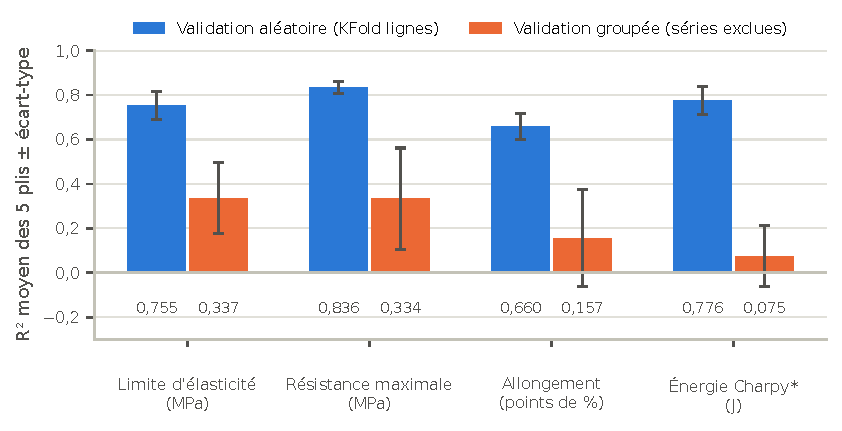
\includegraphics[width=\textwidth]{res_synthese_r2}
\caption{Résultat principal : $R^2$ moyen ($\pm$ écart-type sur 5 plis) de la
procédure supervisée avec sélection interne de la famille, configuration
16/médiane. Bleu : validation aléatoire ; orange : validation groupée.}
\label{fig:synthese}
\end{figure}

\begin{table}[htbp]
\centering
\small
\caption{Procédure supervisée avec sélection interne, configuration 16/médiane :
moyennes $\pm$ écart-type sur 5 plis externes, et MAE relative à la médiane de la cible.}
\label{tab:synthese}
\footnotesize
\setlength{\tabcolsep}{4pt}
\begin{tabular}{@{}l rrr rrr@{}}
\toprule
 & \multicolumn{3}{c}{Validation aléatoire} & \multicolumn{3}{c}{Validation groupée} \\
\cmidrule(lr){2-4}\cmidrule(lr){5-7}
Cible & MAE & MAE rel. & $R^2$ & MAE & MAE rel. & $R^2$ \\
\midrule
\YS{} (MPa)               & 31,630 $\pm$ 4,114 & 6,4\,\%  & 0,755 $\pm$ 0,063 & 56,757 $\pm$ 12,398 & 11,4\,\% & 0,337 $\pm$ 0,161 \\
\UTS{} (MPa)              & 23,861 $\pm$ 0,906 & 4,1\,\%  & 0,836 $\pm$ 0,027 & 54,344 $\pm$ 13,181 & 9,4\,\%  & 0,334 $\pm$ 0,228 \\
Allongement (pts de \%)   & 2,054 $\pm$ 0,239  & 7,7\,\%  & 0,660 $\pm$ 0,058 & 3,517 $\pm$ 0,516   & 13,2\,\% & 0,157 $\pm$ 0,220 \\
\charpy{} (J)             & 16,461 $\pm$ 1,161 & 16,5\,\% & 0,776 $\pm$ 0,062 & 35,752 $\pm$ 11,863 & 35,8\,\% & 0,075 $\pm$ 0,138 \\
\bottomrule
\end{tabular}
\end{table}

\paragraph{Lecture.} En validation aléatoire, l'erreur typique est de
\textbf{32\,MPa sur \YS{} et 24\,MPa sur \UTS}, soit 4 à 6\,\% de la valeur
médiane, et les $R^2$ dépassent 0,75 pour \YS, \UTS{} et Charpy. Par rapport à la
référence médiane, la MAE baisse de 55\,\% (\YS), 65\,\% (\UTS), 49\,\%
(allongement) et 55\,\% (Charpy). En validation groupée, les mêmes procédures
perdent une grande partie de leur pouvoir prédictif : la MAE ne baisse plus que
de 19\,\% (\YS), 25\,\% (\UTS), 14\,\% (allongement) et 1\,\% (Charpy) par rapport à
la référence. L'écart entre les deux scénarios est le résultat le plus
important du projet ; la \cref{sec:diag} en analyse les causes.

\subsection{Comparaison des familles de modèles}

Pour comprendre d'où viennent ces scores, chaque famille est aussi évaluée
séparément, avec ses hyperparamètres réglés en interne
(\cref{fig:familles}, \cref{tab:familles}).

\begin{figure}[htbp]
\centering
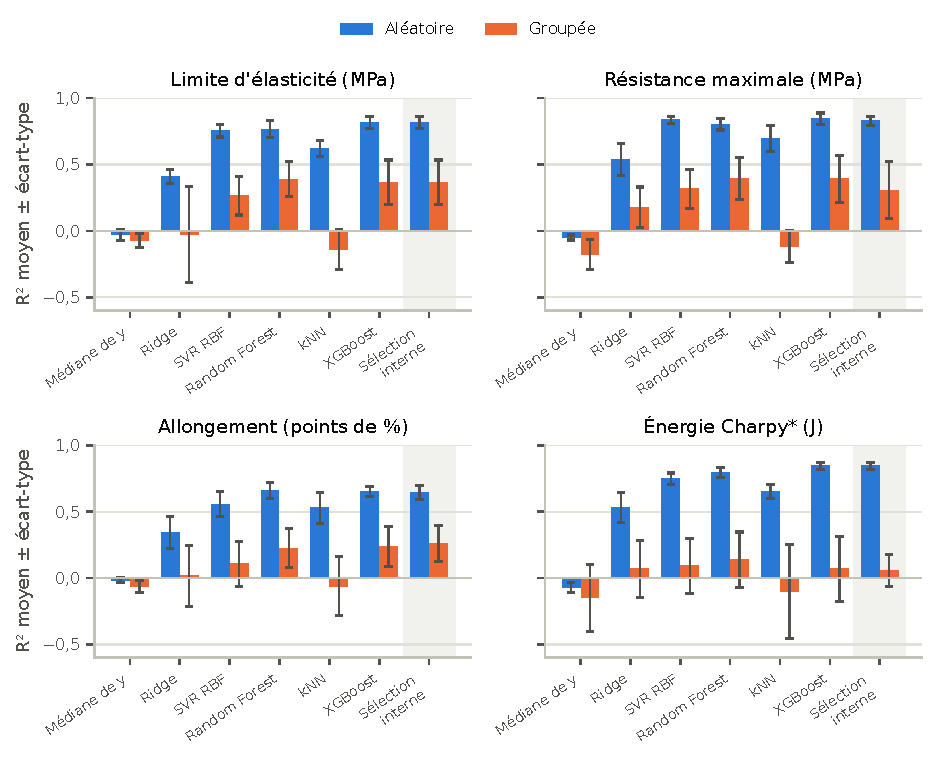
\includegraphics[width=\textwidth]{res_familles_r2}
\caption{$R^2$ moyen ($\pm$ écart-type) de chaque famille, configuration 16/médiane,
validations aléatoire et groupée. La dernière colonne (fond gris) est la procédure
de sélection interne de la famille.}
\label{fig:familles}
\end{figure}

\begin{table}[htbp]
\centering
\small
\caption{MAE moyenne et $R^2$ moyen par famille, configuration 16/médiane
(A : validation aléatoire ; G : validation groupée). En gras : meilleure famille par colonne.}
\label{tab:familles}
\setlength{\tabcolsep}{4pt}
\begin{tabular}{@{}l rr rr rr rr@{}}
\toprule
 & \multicolumn{2}{c}{\YS{} (MPa)} & \multicolumn{2}{c}{\UTS{} (MPa)} & \multicolumn{2}{c}{Allong. (pts)} & \multicolumn{2}{c}{\charpy{} (J)} \\
\cmidrule(lr){2-3}\cmidrule(lr){4-5}\cmidrule(lr){6-7}\cmidrule(lr){8-9}
Famille & A & G & A & G & A & G & A & G \\
\midrule
\multicolumn{9}{@{}l}{\emph{MAE}} \\
Médiane de $y$  & 70,03 & 70,45 & 68,88 & 72,66 & 4,02 & 4,09 & 36,76 & 36,04 \\
Ridge           & 54,05 & 69,39 & 44,32 & 61,90 & 3,01 & 3,66 & 26,91 & 34,75 \\
SVR RBF         & 31,75 & 59,35 & \meilleur{23,86} & 52,86 & 2,27 & 3,67 & 17,39 & 35,96 \\
Forêt aléatoire & \meilleur{31,24} & \meilleur{54,14} & 26,91 & \meilleur{48,91} & \meilleur{2,05} & \meilleur{3,34} & \meilleur{16,10} & \meilleur{33,03} \\
$k$NN           & 38,14 & 73,50 & 33,45 & 68,54 & 2,42 & 3,98 & 19,25 & 35,73 \\
\addlinespace
\multicolumn{9}{@{}l}{\emph{$R^2$}} \\
Médiane de $y$  & $-0{,}031$ & $-0{,}073$ & $-0{,}050$ & $-0{,}180$ & $-0{,}015$ & $-0{,}062$ & $-0{,}069$ & $-0{,}149$ \\
Ridge           & 0,412 & $-0{,}025$ & 0,538 & 0,179 & 0,345 & 0,016 & 0,529 & 0,069 \\
SVR RBF         & 0,754 & 0,264 & \meilleur{0,836} & 0,316 & 0,556 & 0,106 & 0,749 & 0,091 \\
Forêt aléatoire & \meilleur{0,765} & \meilleur{0,390} & 0,805 & \meilleur{0,394} & \meilleur{0,660} & \meilleur{0,226} & \meilleur{0,795} & \meilleur{0,138} \\
$k$NN           & 0,619 & $-0{,}140$ & 0,697 & $-0{,}115$ & 0,530 & $-0{,}060$ & 0,651 & $-0{,}099$ \\
\bottomrule
\end{tabular}
\end{table}

\paragraph{Analyse par famille.}
\begin{itemize}
  \item \textbf{Référence médiane.} Son $R^2$ est légèrement négatif, comme attendu : prédire la médiane du train est un peu moins bon que prédire la moyenne de la validation. Elle fixe le plancher.
  \item \textbf{Ridge.} Elle capte une partie du signal en aléatoire ($R^2$ de 0,35 à 0,54), mais presque rien en groupé. Une relation \emph{linéaire} globale ne suffit pas à décrire les propriétés.
  \item \textbf{SVR RBF et forêt aléatoire.} Ce sont les deux meilleures familles. La SVR est la meilleure pour \UTS{} en aléatoire ; la forêt est la meilleure partout ailleurs et la plus robuste en validation groupée. Les non-linéarités et interactions sont donc importantes.
  \item \textbf{$k$NN.} Très correct en aléatoire ($R^2$ de 0,53 à 0,70) mais \emph{négatif} en groupé. C'est un signal clair : une méthode purement locale prédit bien lorsqu'un voisin de la même série est présent dans le train, et échoue lorsque ce n'est plus le cas.
\end{itemize}

\begin{precaution}
La forêt aléatoire isolée peut afficher un meilleur score externe que la
procédure de sélection interne (par exemple 0,390 contre 0,337 pour \YS{} en
groupé). Choisir la forêt \emph{après} avoir lu ce tableau reviendrait à
sélectionner sur la validation : seul le score de la sélection interne est une
estimation honnête de la procédure complète.
\end{precaution}

\subsection{Familles et hyperparamètres sélectionnés}

La sélection interne peut choisir une famille différente selon le pli. Les
\cref{tab:selection_aleatoire,tab:selection_groupee} détaillent ces choix.

\begin{table}[htbp]
\centering
\small
\caption{Validation aléatoire : famille et hyperparamètres choisis par la MAE
interne dans chaque pli externe, et scores externes obtenus.}
\label{tab:selection_aleatoire}
\setlength{\tabcolsep}{4pt}
\begin{tabular}{@{}l c l l r r@{}}
\toprule
Cible & Pli & Famille & Hyperparamètres & MAE & $R^2$ \\
\midrule
\YS     & 0 & SVR RBF & $C=10$, $\varepsilon=0{,}05$, $\gamma=0{,}05$ & 28,27 & 0,769 \\
        & 1 & Forêt   & feuille 1, prof. libre, \texttt{mf} 0,5 & 29,26 & 0,817 \\
        & 2 & Forêt   & feuille 1, prof. libre, \texttt{mf} 0,5 & 35,67 & 0,671 \\
        & 3 & SVR RBF & $C=10$, $\varepsilon=0{,}05$, $\gamma$=scale & 28,42 & 0,807 \\
        & 4 & SVR RBF & $C=10$, $\varepsilon=0{,}05$, $\gamma$=scale & 36,54 & 0,710 \\
\midrule
\UTS    & 0--4 & SVR RBF & $C=10$, $\varepsilon=0{,}05$, $\gamma \in \{0{,}05;\text{scale}\}$ & 23,1--25,4 & 0,814--0,871 \\
\midrule
Allong. & 0--4 & Forêt & feuille 1, prof. libre, \texttt{mf} $\in\{0{,}5; 1\}$ & 1,84--2,42 & 0,569--0,728 \\
\midrule
Charpy  & 0, 1, 3, 4 & Forêt & feuille 1, prof. libre, \texttt{mf} $\in\{0{,}5; 1\}$ & 14,9--17,5 & 0,756--0,849 \\
        & 2 & SVR RBF & $C=100$, $\varepsilon=0{,}05$, $\gamma=0{,}05$ & 17,51 & 0,683 \\
\bottomrule
\end{tabular}
\end{table}

\begin{table}[htbp]
\centering
\small
\caption{Validation groupée : famille et hyperparamètres choisis par la MAE
interne dans chaque pli externe, et scores externes obtenus.}
\label{tab:selection_groupee}
\setlength{\tabcolsep}{4pt}
\begin{tabular}{@{}l c l l r r@{}}
\toprule
Cible & Pli & Famille & Hyperparamètres & MAE & $R^2$ \\
\midrule
\YS     & 0 & Forêt   & feuille 2, prof. libre, \texttt{mf} 0,5 & 43,62 & 0,472 \\
        & 1 & Forêt   & feuille 1, prof. libre, \texttt{mf} 0,5 & 68,48 & 0,204 \\
        & 2 & SVR RBF & $C=10$, $\varepsilon=0{,}05$, $\gamma=0{,}05$ & 49,94 & 0,273 \\
        & 3 & Forêt   & feuille 1, prof. 10, \texttt{mf} 0,5 & 50,28 & 0,543 \\
        & 4 & SVR RBF & $C=10$, $\varepsilon=0{,}2$, $\gamma=0{,}05$ & 71,46 & 0,191 \\
\midrule
\UTS    & 0 & Ridge   & $\alpha=100$ & 74,90 & 0,038 \\
        & 1 & Forêt   & feuille 1, prof. libre, \texttt{mf} 0,5 & 49,49 & 0,155 \\
        & 2 & SVR RBF & $C=10$, $\varepsilon=0{,}05$, $\gamma=0{,}05$ & 38,76 & 0,399 \\
        & 3 & Forêt   & feuille 2, prof. 10, \texttt{mf} 0,5 & 52,60 & 0,555 \\
        & 4 & Forêt   & feuille 2, prof. libre, \texttt{mf} 0,5 & 55,98 & 0,523 \\
\midrule
Allong. & 0, 1, 3 & Forêt & \texttt{mf} 0,5, feuille 5/2/5 & 2,86--3,63 & 0,166--0,468 \\
        & 2, 4 & SVR RBF & $\varepsilon=0{,}2$, $\gamma=0{,}05$, $C=1$/$10$ & 3,61--4,25 & $-0{,}080$--$-0{,}022$ \\
\midrule
Charpy  & 0, 1 & SVR RBF & $C=1$, $\varepsilon=0{,}2$, $\gamma=0{,}05$ & 31,00 / 27,33 & $-0{,}038$ / 0,222 \\
        & 2, 4 & Médiane de $y$ & -- & 24,24 / 44,12 & $-0{,}034$ / $-0{,}006$ \\
        & 3 & Forêt   & feuille 1, prof. libre, \texttt{mf} 1 & 52,09 & 0,228 \\
\bottomrule
\end{tabular}
\end{table}

Plusieurs enseignements ressortent. En aléatoire, les choix sont
\textbf{stables} : SVR ($C=10$, $\varepsilon=0{,}05$) pour \UTS{} dans les cinq
plis, forêt à feuilles de taille 1 pour l'allongement. Les modèles peu
régularisés sont préférés, ce qui est cohérent avec un contexte où des voisins
très proches existent dans le train. En groupé, les choix sont \textbf{instables}
--- Ridge, SVR ou forêt pour \UTS{} selon le pli --- et la boucle interne
retient même la \textbf{référence médiane} dans deux plis Charpy : en l'absence
de séries connues, aucun modèle ne bat de façon fiable la constante pour cette
cible. Cette instabilité illustre l'incertitude du transfert entre séries.

\subsection{Prédictions et observations}

La \cref{fig:obs_pred} compare les prédictions hors pli aux valeurs observées.

\begin{figure}[htbp]
\centering
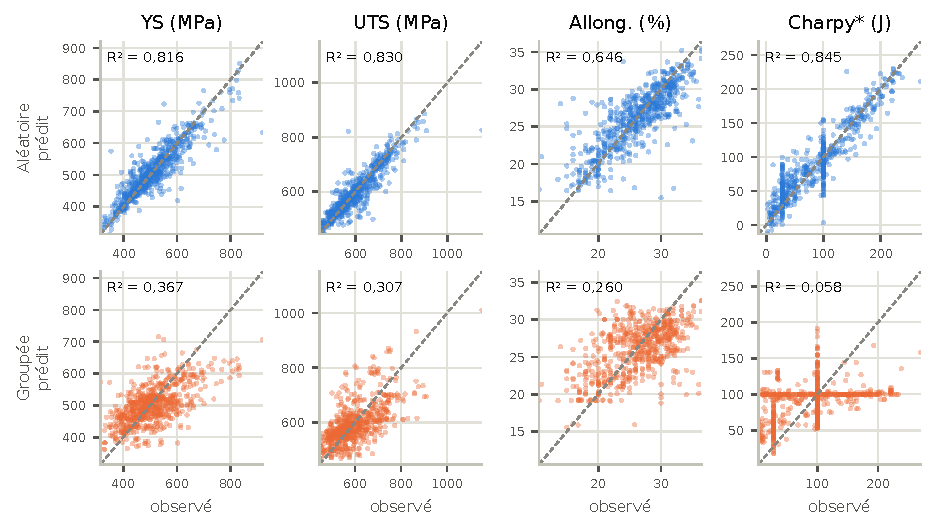
\includegraphics[width=\textwidth]{res_observe_predit}
\caption{Valeurs observées et prédites hors pli (OOF) par la procédure de
sélection interne, configuration 16/médiane. Haut : validation aléatoire ; bas :
validation groupée. La diagonale pointillée correspond à une prédiction parfaite.}
\label{fig:obs_pred}
\end{figure}

En validation aléatoire, les points suivent la diagonale. En validation groupée,
le nuage est \textbf{aplati} : les prédictions restent proches de la moyenne et
les fortes valeurs de \YS{} et \UTS{} sont sous-estimées. Pour Charpy, on
distingue des bandes verticales à 28 et 100\,J : pour ces couples, le modèle
prédit des énergies très variées alors que l'énergie observée est fixée par le
protocole, ce qui est cohérent avec l'hypothèse de températures de transition.

\subsection{Modèles réentraînés pour l'inférence}

Une fois l'évaluation terminée, chaque famille est réglée par une nouvelle CV5
sur \emph{tous} les labels (aléatoire, graine 1042, ou par groupes), puis
réentraînée. La famille de plus faible MAE de sélection est retenue par cible
(\cref{tab:modeles_finaux}). Ces MAE de sélection sont optimistes et \textbf{ne
remplacent pas} les scores imbriqués ; ces modèles ont vu tous les labels et ne
servent jamais à scorer les plis.

\begin{table}[htbp]
\centering
\small
\caption{Modèles supervisés réentraînés sur tous les labels, retenus pour l'inférence.}
\label{tab:modeles_finaux}
\begin{tabular}{@{}l l l r l@{}}
\toprule
CV de choix & Cible & Famille & MAE de sélection & Hyperparamètres \\
\midrule
Aléatoire & \YS     & SVR RBF & 31,228 & $C=10$, $\varepsilon=0{,}05$, $\gamma$=scale \\
          & \UTS    & SVR RBF & 24,060 & $C=10$, $\varepsilon=0{,}05$, $\gamma=0{,}05$ \\
          & Allong. & Forêt   & 1,940  & feuille 1, prof. libre, \texttt{mf} 0,5 \\
          & Charpy  & Forêt   & 15,387 & feuille 1, prof. libre, \texttt{mf} 1 \\
\midrule
Groupée   & \YS     & Forêt   & 58,695 & feuille 2, prof. libre, \texttt{mf} 0,5 \\
          & \UTS    & SVR RBF & 46,555 & $C=10$, $\varepsilon=0{,}05$, $\gamma=0{,}05$ \\
          & Allong. & Forêt   & 3,282  & feuille 1, prof. libre, \texttt{mf} 0,5 \\
          & Charpy  & Forêt   & 32,375 & feuille 1, prof. 10, \texttt{mf} 0,5 \\
\bottomrule
\end{tabular}
\end{table}

Au total, \textbf{80 pipelines supervisées} sont exportées (40 par protocole :
20 modèles de plis externes et 20 réapprentissages complets), avec leur
prétraitement, leurs métadonnées (entrées, unités, identifiants du train,
paramètres, versions) et leur empreinte SHA-256. Toutes ont été rechargées dans
un processus Python neuf et les modèles de plis reproduisent exactement leurs
prédictions hors pli.

\begin{aretenir}
\begin{itemize}[leftmargin=1.2em]
  \item Configuration initiale 13/itérative : gains modestes, $R^2 \leq 0{,}19$ en validation groupée.
  \item Configuration 16/médiane : $R^2$ de \textbf{0,66 à 0,84 en aléatoire}, mais \textbf{0,08 à 0,34 en groupé}.
  \item \textbf{Forêt aléatoire et SVR RBF} sont les meilleures familles ; le $k$NN s'effondre dès que la série est absente.
  \item Les choix internes sont stables en aléatoire, instables en groupé.
\end{itemize}
\end{aretenir}

% =====================================================================
%  8. Diagnostics et explicabilité
% =====================================================================
\clearpage
\section{Diagnostics des performances et explicabilité}
\label{sec:diag}

Le premier benchmark (\cref{tab:bench13}) a produit des $R^2$ faibles en
validation groupée. Plutôt que d'essayer des modèles au hasard, le notebook
\notebook{04\_diagnostics.ipynb} a cherché à \emph{comprendre} ces scores. Le
protocole des diagnostics a été fixé avant leur calcul ; il réutilise les mêmes
labels, la même cohorte et les mêmes plis. Ces analyses sont \textbf{rétrospectives} :
elles ne constituent pas une validation indépendante des choix qu'elles ont motivés.

\subsection{Les modèles apprennent, mais transfèrent mal}

Le \cref{tab:ecart_train} compare les scores sur le train et en validation
groupée pour le benchmark 13/itérative.

\begin{table}[htbp]
\centering
\small
\caption{Écart entre entraînement et validation groupée, forêt aléatoire du benchmark 13/itérative.}
\label{tab:ecart_train}
\begin{tabular}{@{}lrrrr@{}}
\toprule
Cible & MAE train & MAE validation & $R^2$ train & $R^2$ validation \\
\midrule
\YS{} (MPa)             & 30,08 & 65,88 & 0,795 & 0,079 \\
\UTS{} (MPa)            & 23,79 & 57,65 & 0,842 & 0,194 \\
Allongement (pts de \%) & 1,33  & 3,56  & 0,859 & 0,125 \\
\charpy{} (J)           & 8,40  & 34,71 & 0,941 & 0,017 \\
\bottomrule
\end{tabular}
\end{table}

La forêt reproduit bien le train ($R^2$ de 0,80 à 0,94) mais généralise mal aux
séries absentes. Les modèles linéaires ont aussi un faible $R^2$ d'entraînement
(0,18 à 0,27 pour Ridge) : ajouter de la capacité non linéaire ne suffit pas.
De plus, les prédictions sont \textbf{comprimées} : l'écart-type des prédictions
vaut environ 0,53 fois celui des observations pour \YS{} et Charpy, 0,68 pour
\UTS{} et 0,64 pour l'allongement ; les soudures très résistantes ou très
tenaces sont sous-estimées.

\subsection{Une grande part de l'erreur vient des séries}

L'erreur quadratique totale peut se décomposer exactement en une part due au
\textbf{biais moyen de chaque série} et une part due aux variations à
l'intérieur des séries :
\begin{equation}
  \mathrm{SSE} = \sum_{g}\sum_{i \in g} e_i^2
  = \underbrace{\sum_{g} n_g\, b_g^2}_{\text{décalage des séries}}
  + \underbrace{\sum_{g}\sum_{i \in g}\bigl(e_i - b_g\bigr)^2}_{\text{dispersion interne}},
\end{equation}
où $e_i = \hat{y}_i - y_i$ est l'erreur de la ligne $i$, $n_g$ l'effectif de la
série $g$ et $b_g = \frac{1}{n_g}\sum_{i\in g} e_i$ son biais moyen.

\begin{table}[htbp]
\centering
\small
\caption{Décomposition de l'erreur de la forêt du benchmark 13/itérative (prédictions OOF réunies).}
\label{tab:decomposition}
\begin{tabularx}{\textwidth}{@{}l C C C C C@{}}
\toprule
Cible & Variance entre séries (\% de SST) & Part de SSE due au biais des séries & $R^2$ OOF & RMSE OOF & RMSE requise pour $R^2 = 0{,}5$ \\
\midrule
\YS{} (MPa)       & 48,0\,\% & 56,4\,\% & 0,091 & 87,7 & 65,0 \\
\UTS{} (MPa)      & 54,9\,\% & 50,6\,\% & 0,280 & 75,9 & 63,3 \\
Allongement (pts) & 54,4\,\% & 50,0\,\% & 0,156 & 4,48 & 3,45 \\
\charpy{} (J)     & 29,1\,\% & 36,5\,\% & 0,116 & 47,5 & 35,7 \\
\bottomrule
\end{tabularx}
\end{table}

Le \cref{tab:decomposition} montre que \textbf{la moitié environ de l'erreur
quadratique} provient de décalages de niveau entre séries : le modèle se trompe
de façon systématique sur une série entière. La \cref{fig:biais} donne les séries
qui concentrent le plus d'erreur. Les biais sont majoritairement négatifs pour la
résistance : les séries très résistantes (par exemple \texttt{SurianEtAl-C-1991},
\texttt{Birmingham}, \texttt{Sw\&Rog-1973}) sont sous-estimées de 170 à 240\,MPa.

\begin{figure}[htbp]
\centering
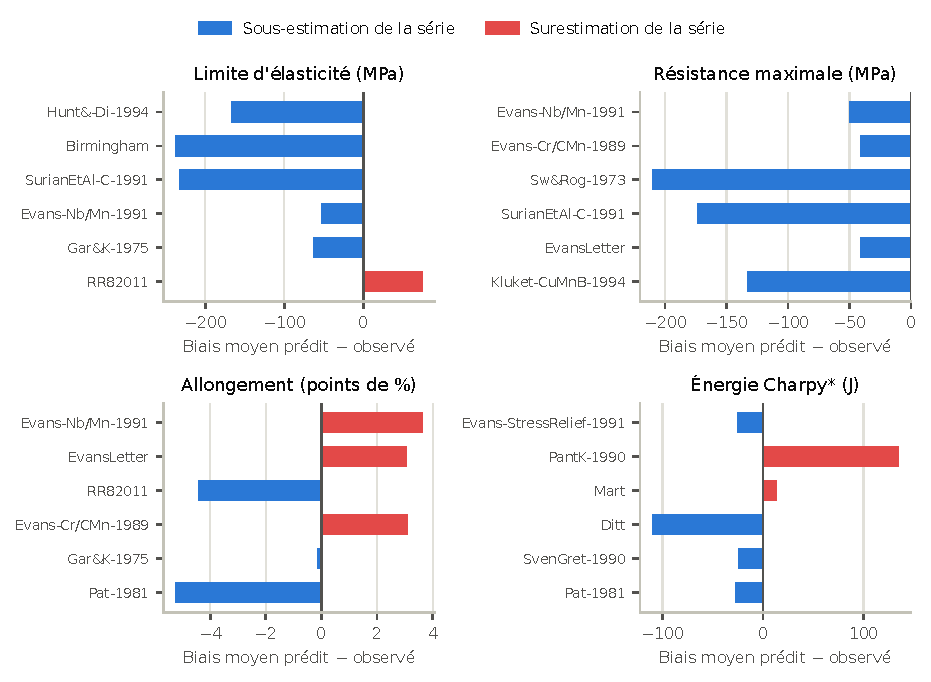
\includegraphics[width=\textwidth]{diag_biais_series}
\caption{Biais moyen (prédit $-$ observé) des six séries qui contribuent le plus à
l'erreur quadratique, forêt du benchmark 13/itérative, validation groupée.}
\label{fig:biais}
\end{figure}

L'examen de cas concrets éclaire ces décalages. La ligne 722
(\texttt{Evans-AlEl9Cr1Mo-1994}) contient 3,01\,\% de Ni et 9,17\,\% de Cr ; son
\UTS{} observée vaut 1\,151\,MPa contre 729\,MPa prédits. La ligne 1\,209
(\texttt{PantK-1990}) contient 8,7\,\% de Cr ; son énergie Charpy observée est de
8\,J contre 159\,J prédits. Or Ni, Cr et Mo \emph{ne faisaient pas partie} des
13 entrées. Ces exemples suggèrent une information omise, que l'extension à
16 entrées teste directement (\cref{subsec:sensibilites}).

\subsection{Domaine des entrées et rôle de l'imputation}

Le \cref{tab:domaine} compare la MAE selon trois indicateurs : présence d'une
entrée imputée, entrée hors des plages observées dans le train, procédé absent
du train.

\begin{table}[htbp]
\centering
\small
\caption{MAE de la forêt (benchmark 13/itérative) selon l'appartenance au domaine du train.}
\label{tab:domaine}
\begin{tabular}{@{}l rr rr rr@{}}
\toprule
 & \multicolumn{2}{c}{Entrée imputée} & \multicolumn{2}{c}{Hors plages du train} & \multicolumn{2}{c}{Procédé inconnu} \\
\cmidrule(lr){2-3}\cmidrule(lr){4-5}\cmidrule(lr){6-7}
Cible & non & oui & non & oui & non & oui \\
\midrule
\YS{} (MPa)       & 72,5 & 57,4 & 65,0 & 73,2 & 64,4 & 102,4 \\
\UTS{} (MPa)      & 58,5 & 53,5 & 54,9 & 64,0 & 54,6 & 95,3 \\
Allongement (pts) & 3,64 & 3,44 & 3,67 & 2,99 & 3,50 & 4,29 \\
\charpy{} (J)     & 33,5 & 37,1 & 28,2 & 52,8 & 32,9 & 45,2 \\
\bottomrule
\end{tabular}
\end{table}

Deux constats en ressortent. D'abord, les lignes avec une entrée imputée
\textbf{ne sont pas systématiquement moins bien prédites} ; pour \YS{} elles le
sont même mieux. L'hypothèse \og l'imputation explique tout \fg{} est donc
contredite. Ensuite, sortir du domaine du train dégrade nettement Charpy
(MAE de 52,8\,J contre 28,2\,J, corrélation de rang erreur/distance 0,41), et un
procédé inconnu du train dégrade fortement \YS{} et \UTS{} (MAE
d'environ 100\,MPa). Ces comparaisons sont descriptives et confondues par les
séries.

\subsection{Sensibilités : entrées et méthode d'imputation}
\label{subsec:sensibilites}

Pour isoler les deux facteurs (nombre d'entrées et imputation), les six
combinaisons \{11, 13, 16 entrées\} $\times$ \{médiane, itérative\} ont été
évaluées avec les quatre familles, les grilles du notebook 03 et les mêmes plis
groupés : 480 évaluations prévues. \textbf{436 ont abouti} ; l'imputation
itérative à 16 entrées \textbf{n'a pas convergé} dans 11 contextes cible/pli
(\YS{} pli 4 ; \UTS{} plis 3--4 ; allongement plis 2--4 ; Charpy tous les plis),
rendant 44 évaluations indisponibles. Conformément au protocole, aucun repli
silencieux n'a été appliqué.

\begin{figure}[htbp]
\centering
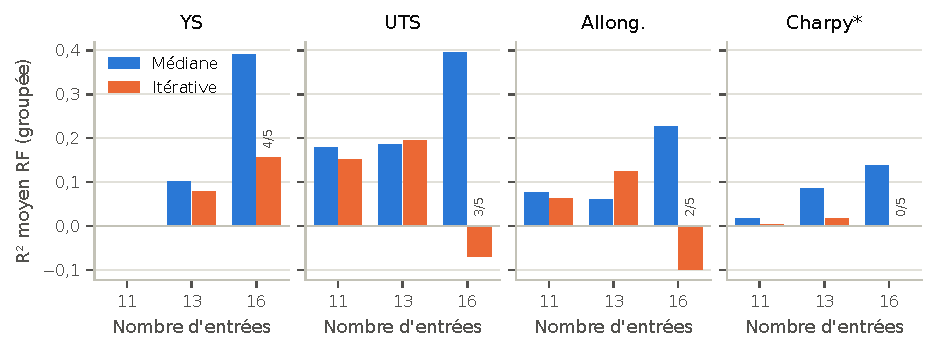
\includegraphics[width=\textwidth]{diag_sensibilites_rf}
\caption{$R^2$ moyen de la forêt aléatoire en validation groupée selon le nombre
d'entrées et l'imputation. Les mentions \og $k$/5 \fg{} signalent les scénarios
où seuls $k$ plis sur 5 ont abouti (non comparables aux scénarios complets).}
\label{fig:sensibilites}
\end{figure}

\begin{table}[htbp]
\centering
\small
\caption{Forêt aléatoire en validation groupée : MAE et $R^2$ moyens selon le
schéma et l'imputation (plis aboutis sur 5 entre parenthèses lorsque incomplets).}
\label{tab:sensibilites}
\setlength{\tabcolsep}{4.5pt}
\begin{tabular}{@{}l l rr rr rr rr@{}}
\toprule
 & & \multicolumn{2}{c}{\YS{} (MPa)} & \multicolumn{2}{c}{\UTS{} (MPa)} & \multicolumn{2}{c}{Allong. (pts)} & \multicolumn{2}{c}{\charpy{} (J)} \\
\cmidrule(lr){3-4}\cmidrule(lr){5-6}\cmidrule(lr){7-8}\cmidrule(lr){9-10}
Entrées & Imputation & MAE & $R^2$ & MAE & $R^2$ & MAE & $R^2$ & MAE & $R^2$ \\
\midrule
11 & médiane   & 68,98 & 0,000 & 57,31 & 0,179 & 3,69 & 0,076 & 35,14 & 0,018 \\
11 & itérative & 69,14 & $-0{,}001$ & 58,38 & 0,151 & 3,68 & 0,063 & 34,71 & 0,002 \\
13 & médiane   & 64,98 & 0,102 & 57,84 & 0,185 & 3,74 & 0,060 & 33,70 & 0,084 \\
13 & itérative & 65,88 & 0,079 & 57,65 & 0,194 & 3,56 & 0,125 & 34,71 & 0,017 \\
16 & médiane   & \meilleur{54,14} & \meilleur{0,390} & \meilleur{48,91} & \meilleur{0,394} & \meilleur{3,34} & \meilleur{0,226} & \meilleur{33,03} & \meilleur{0,138} \\
16 & itérative & 60,80 (4) & 0,156 & 57,32 (3) & $-0{,}069$ & 3,97 (2) & $-0{,}099$ & -- (0) & -- \\
\bottomrule
\end{tabular}
\end{table}

Le passage de 13 à 16 entrées à imputation médiane identique produit un
\textbf{gain apparié de MAE OOF} de la forêt (bootstrap par groupes, 2\,000 tirages) :
\begin{itemize}
  \item \YS{} : \textbf{11,06\,MPa}, intervalle [3,09 ; 20,19] ;
  \item \UTS{} : \textbf{8,80\,MPa}, intervalle [2,38 ; 15,40] ;
  \item allongement : 0,39 point, intervalle [$-0{,}05$ ; 0,87] ;
  \item Charpy : 0,65\,J, intervalle [$-0{,}21$ ; 1,64].
\end{itemize}
Les intervalles de \YS{} et \UTS{} excluent zéro : Ni, Cr et Mo apportent une
information prédictive réelle sur la résistance. Pour l'allongement et Charpy,
le gain n'est pas établi.

Un contrôle complémentaire a masqué 20\,\% des valeurs \emph{observées} de Ni,
Cr et Mo en validation, puis comparé leur reconstruction. L'itérative ne domine
pas : pour Charpy, l'erreur absolue moyenne sur Cr vaut 4,79\,\% massique avec
l'itérative contre 1,50\,\% avec la médiane, sur les mêmes cellules. Une
imputation plus sophistiquée ne garantit donc pas une meilleure reconstruction
hors série.

\begin{decision}
La configuration de travail devient \textbf{16 entrées + médiane} : gain établi
pour \YS{} et \UTS, convergence garantie, aucune perte de lignes. Elle reste un
\emph{candidat} à valider sur des séries indépendantes, car elle a été choisie
après observation des scores.
\end{decision}

\paragraph{Sélection conjointe interne.} Pour mesurer ce que coûterait un choix
automatique, une procédure a aussi choisi \emph{dans la boucle interne} le schéma,
l'imputation, la famille et les hyperparamètres. Ses $R^2$ externes sont 0,337
(\YS), 0,334 (\UTS), 0,164 (allongement) et $-0{,}100$ (Charpy), inférieurs à ceux
de la forêt 16/médiane fixée : la sélection fluctue d'un pli à l'autre, signe
de la fragilité du transfert. Enfin, régler les hyperparamètres par MSE plutôt
que par MAE ne change presque rien (par exemple $R^2$ de la forêt pour \UTS{} :
0,206 contre 0,194).

\subsection{Effet du mode de découpage}
\label{subsec:decoupages}

Si la difficulté vient des séries, le même modèle devrait obtenir des scores très
différents selon ce qui est séparé. Une forêt \emph{identique}, sans réglage
(300 arbres, feuille 2, profondeur libre, toutes les variables, graine 42), a été
évaluée avec trois découpages (\cref{fig:decoupages}) : lignes aléatoires,
conditions de soudage séparées (même signature des 16 entrées et du procédé), et
séries séparées.

\begin{figure}[htbp]
\centering
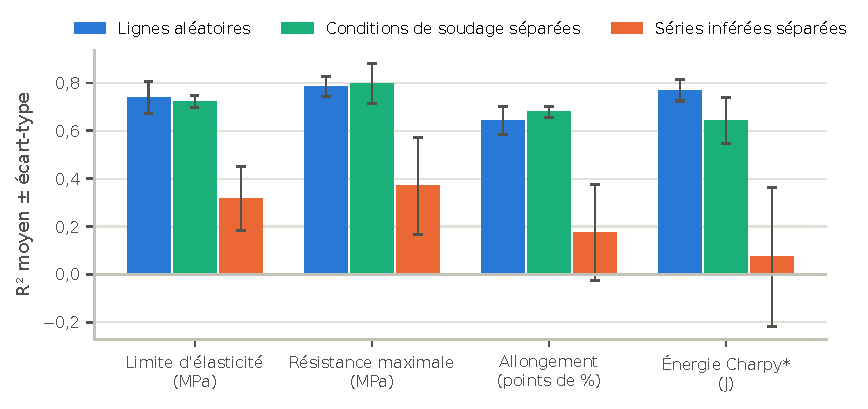
\includegraphics[width=\textwidth]{diag_decoupages_rf}
\caption{Même forêt aléatoire, sans réglage, configuration 16/médiane, sous trois
découpages. Séparer des conditions de soudage répétées change peu le score ;
séparer des séries entières le fait chuter.}
\label{fig:decoupages}
\end{figure}

\begin{table}[htbp]
\centering
\small
\caption{$R^2$ moyen de la forêt fixe selon le découpage, et structure des séries.}
\label{tab:decoupages}
\begin{tabular}{@{}l rrr rr@{}}
\toprule
 & \multicolumn{3}{c}{$R^2$ moyen selon le découpage} & \multicolumn{2}{c}{Structure des séries} \\
\cmidrule(lr){2-4}\cmidrule(lr){5-6}
Cible & Lignes & Conditions & Séries & Séries multi-conditions & Variance entre séries \\
\midrule
\YS     & 0,739 & 0,722 & 0,318 & 37 / 40 & 48,0\,\% \\
\UTS    & 0,786 & 0,797 & 0,370 & 36 / 39 & 54,9\,\% \\
Allong. & 0,644 & 0,680 & 0,175 & 33 / 34 & 54,4\,\% \\
Charpy  & 0,769 & 0,643 & 0,074 & 23 / 24 & 29,1\,\% \\
\bottomrule
\end{tabular}
\end{table}

Pour la traction, séparer les conditions répétées ne fait presque pas baisser le
score : le problème n'est pas une simple répétition de mesures identiques. En
revanche, séparer des séries divise le $R^2$ par deux à quatre. Presque toutes
les séries contiennent plusieurs conditions de soudage (37 sur 40 pour \YS) : ce
ne sont pas des doublons, mais des études cohérentes dont le \og niveau \fg{} est
propre. Un test de permutation (999 permutations) confirme que la part de
variance des cibles portée par les séries (29 à 55\,\%) est très supérieure à ce
qu'on obtiendrait par hasard (4 à 8\,\% au 95\textsuperscript{e} centile ; $p = 0{,}001$).
Ce test reste exploratoire : les répétitions limitent l'échangeabilité des lignes.
Pour Charpy, 65\,\% des points de validation aléatoire partagent la condition de
soudage d'un point du train (à une autre température), ce qui explique son
$R^2$ aléatoire élevé.

\subsection{Quantité de données : courbes d'apprentissage}

La \cref{fig:apprentissage} fait varier la fraction des groupes du train (50, 75 et
100\,\%) sans toucher à la validation, avec deux graines.

\begin{figure}[htbp]
\centering
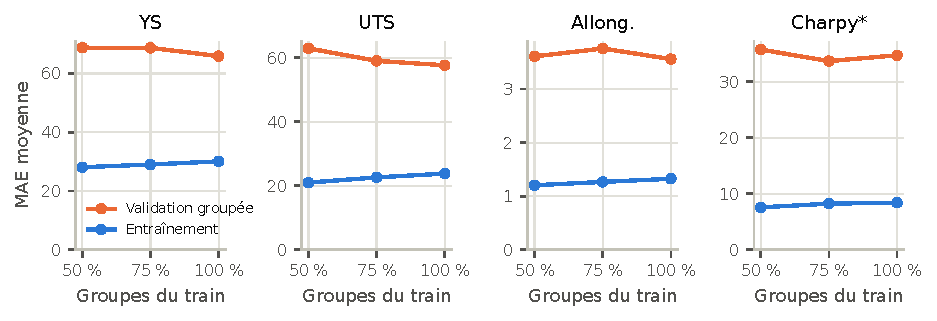
\includegraphics[width=\textwidth]{diag_courbes_apprentissage}
\caption{MAE d'entraînement et de validation groupée de la forêt (benchmark
13/itérative) en fonction de la fraction de groupes d'entraînement utilisée.}
\label{fig:apprentissage}
\end{figure}

\YS{} et \UTS{} profitent de groupes supplémentaires (MAE \UTS{} de 62,9 à
57,7\,MPa), tandis que l'allongement et Charpy ne s'améliorent pas de façon
monotone. Le large écart entre train et validation persiste : davantage de
\emph{séries diverses} semble plus utile que davantage de lignes d'une même série.

\subsection{Explicabilité : quelles informations le modèle utilise-t-il ?}

L'importance par permutation~\cite{breiman_2001,fisher_2019} mesure la hausse de
MAE lorsque l'on mélange aléatoirement une entrée (ou un bloc d'entrées corrélées)
dans la validation, sans réentraîner le modèle. Les blocs sont : composition,
paramètres de soudage, PWHT, procédé et, pour Charpy, température d'essai.

\begin{figure}[htbp]
\centering
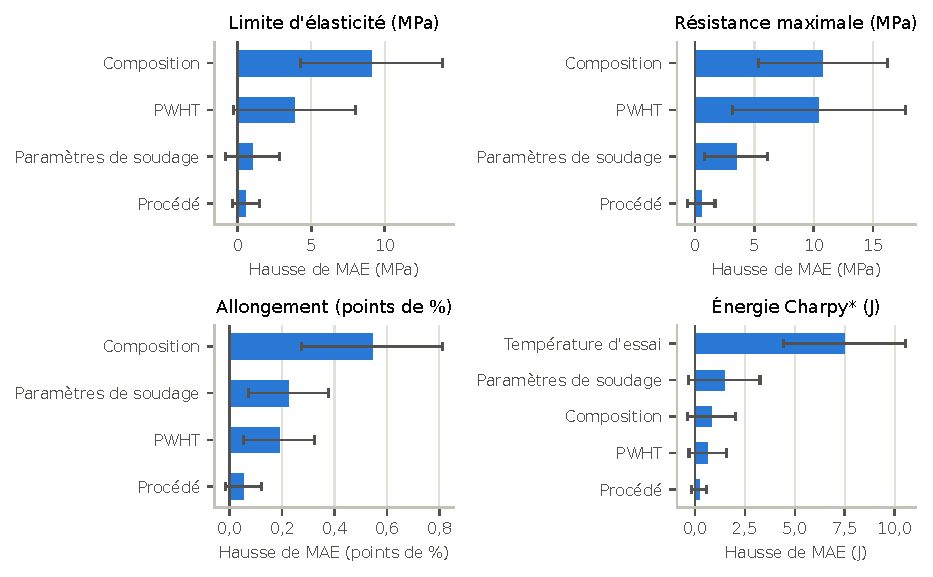
\includegraphics[width=\textwidth]{diag_importance_blocs}
\caption{Importance par permutation de blocs d'entrées (forêt du benchmark
13/itérative, validation groupée, dix permutations par pli). Barres : hausse
moyenne de MAE ; traits : écart-type entre répétitions et plis.}
\label{fig:importance}
\end{figure}

La \cref{fig:importance} indique que la \textbf{composition} et le \textbf{PWHT}
portent l'essentiel de l'information utilisée pour la résistance (hausse de MAE
de 9,1 et 3,9\,MPa pour \YS ; 10,7 et 10,4\,MPa pour \UTS), que la composition
domine pour l'allongement, et que la \textbf{température d'essai} domine pour
Charpy (+7,5\,J). Des contributions locales exactes, calculées le long des chemins
des arbres, reconstruisent chaque prédiction et ont servi à analyser les plus
grosses erreurs ; elles dépendent de l'ordre des coupures et ne sont pas des
valeurs SHAP.

\begin{precaution}
Ces importances décrivent \emph{le comportement du modèle}, pas des effets
physiques causaux. Des entrées corrélées peuvent se substituer l'une à l'autre,
et l'importance d'une variable dans un modèle faible n'établit pas une hiérarchie
métallurgique.
\end{precaution}

\subsection{Audit des protocoles Charpy}
\label{subsec:charpy_audit}

Pour Charpy, les séries ont été confrontées à leurs publications originales,
par correspondance de compositions et de conditions (\cref{tab:charpy_audit}).

\begin{table}[htbp]
\centering
\small
\caption{Correspondance des séries Charpy avec leurs publications originales.}
\label{tab:charpy_audit}
\begin{tabularx}{\textwidth}{@{}l r L@{}}
\toprule
Série & Lignes & Constat \\
\midrule
\texttt{SvenGret-1990}~\cite{svensson_gretoft_1990} & 80 & 16 compositions et conditions concordantes ; énergies mesurées à cinq températures présélectionnées, cinq éprouvettes par température : \textbf{courbes $E(T)$ confirmées} \\
\texttt{Evans-StressRelief-1991}~\cite{evans_1986_sr} & 94 & 16 compositions et six conditions concordantes avec une publication de 1986 (malgré l'année 1991 de l'identifiant) : \textbf{famille de courbes de transition confirmée} \\
\texttt{Evans-Cr/CMn-1989}~\cite{evans_1989_cr} & 31 & 20 compositions concordantes ; la publication présente des températures à 100\,J et les 31 couples valent 100\,J : \textbf{extraction de températures de transition probable} \\
21 autres séries & 656 & Non résolues par leur publication originale \\
\bottomrule
\end{tabularx}
\end{table}

Dans la cohorte, 457 des 861 énergies (53,1\,\%) valent exactement 28 ou 100\,J.
Un point à 100\,J appartient bien à la courbe $E(T)$, mais sa température a été
choisie en fonction de l'énergie : il renseigne la position de la transition,
pas toute la courbe. Mélanger ces règles d'échantillonnage peut modifier la
distribution évaluée. Deux familles confirmées (174 points) ne suffisent pas à
construire une nouvelle validation imbriquée par sources : \textbf{Charpy reste
exploratoire}. L'audit a par ailleurs confirmé que la publication Svensson--Gretoft
exprime Ti/Al/Sn/As/Sb en \% massique, ce qui conforte la quarantaine des unités.

\subsection{Bilan des diagnostics}

\begin{aretenir}
\textbf{Établi :} grand écart train/validation ; environ la moitié de l'erreur
due à des décalages de niveau entre séries ; prédictions comprimées ; apport
réel de Ni/Cr/Mo pour \YS{} et \UTS ; instabilité de l'imputation itérative à
16 entrées ; difficulté accrue hors du domaine du train pour Charpy ; règles
d'échantillonnage Charpy hétérogènes.

\textbf{Plausible mais non isolé :} compositions ou états métallurgiques omis
(Nb, V, Cu, Ti, B\ldots), différences de protocoles entre séries, précision de
transcription des labels.

\textbf{Non démontré :} que l'imputation explique les faibles scores ; qu'un
bruit expérimental plafonne le $R^2$ sous 0,5 ; qu'une ACP ou un modèle
multi-sorties résoudrait le problème ; que retirer les séries difficiles
améliorerait la généralisation.
\end{aretenir}

% =====================================================================
%  9. Résultats semi-supervisés : COREG
% =====================================================================
\clearpage
\section{Résultats semi-supervisés : COREG}
\label{sec:ssl}

COREG (\cref{subsec:coreg_algo}) a été entraîné dans le notebook
\notebook{07\_coreg.ipynb} pour les trois cibles de traction, avec la
configuration 16/médiane, sous les deux protocoles de validation imbriquée et selon
le protocole inductif de la \cref{subsec:inductif}. Tous les vrais labels du train
sont utilisés ; aucun label n'est masqué artificiellement. Charpy n'est pas
concerné, son pool naturel étant vide. Au total : 180 évaluations externes et
576 ajustements COREG (choix internes, réapprentissages complets et sensibilité
aux graines compris).

\subsection{Méthodes comparées}

Pour attribuer correctement un éventuel gain aux pseudo-labels, COREG est comparé
à plusieurs contrôles évalués sur exactement les mêmes observations :
\begin{itemize}
  \item \textbf{moyenne $k$NN L1/L2 au même $k$, sans pseudo-labels} : le contrôle \emph{apparié}, qui ne diffère de COREG que par l'ajout de pseudo-labels ;
  \item \textbf{moyenne $k$NN L1/L2 réglée} : même architecture, $k$ choisi indépendamment ;
  \item \textbf{$k$NN L1 seul} et \textbf{$k$NN L2 seul} ;
  \item \textbf{sélection supervisée} : la procédure de référence de la \cref{subsec:res16}, qui ne sert jamais à initialiser COREG.
\end{itemize}

\subsection{Déroulement de la boucle}

Le \cref{tab:coreg_boucle} résume ce qui se passe dans les cinq ajustements
externes de chaque cible et protocole.

\begin{table}[htbp]
\centering
\small
\caption{Déroulement de COREG dans les cinq plis externes (min--max sur les plis).
\og Pool distinct \fg{} : après déduplication et retrait des représentations déjà
présentes parmi les vrais labels.}
\label{tab:coreg_boucle}
\footnotesize
\setlength{\tabcolsep}{4pt}
\begin{tabular}{@{}l l rrrr l@{}}
\toprule
Protocole & Cible & Pool brut & Pool distinct & Pseudo-labels & Tours & Arrêts \\
\midrule
Aléatoire & \YS     & 679--680 & 224--234 & 118--170 & 61--91 & 5 sans gain positif \\
          & \UTS    & 702--703 & 249--258 & 70--158  & 38--82 & 5 sans gain positif \\
          & Allong. & 739--740 & 275--290 & 52--197  & 29--100 & 4 sans gain, 1 au maximum \\
\midrule
Groupé    & \YS     & 651--696 & 143--240 & 80--200  & 42--100 & 2 sans gain, 2 max., 1 pool épuisé \\
          & \UTS    & 682--742 & 149--270 & 122--200 & 66--100 & 3 sans gain, 2 au maximum \\
          & Allong. & 725--763 & 189--293 & 80--200  & 42--100 & 2 sans gain, 3 au maximum \\
\bottomrule
\end{tabular}
\end{table}

La déduplication réduit fortement le pool : sur environ 700 lignes sans label par
pli, seules 140 à 290 représentations sont réellement nouvelles. Beaucoup de
lignes non étiquetées décrivent des conditions déjà présentes parmi les labels.
La \cref{fig:coreg_iter} montre que chaque tour ajoute presque toujours deux
pseudo-labels (un par régresseur) jusqu'à l'arrêt.

\begin{figure}[htbp]
\centering
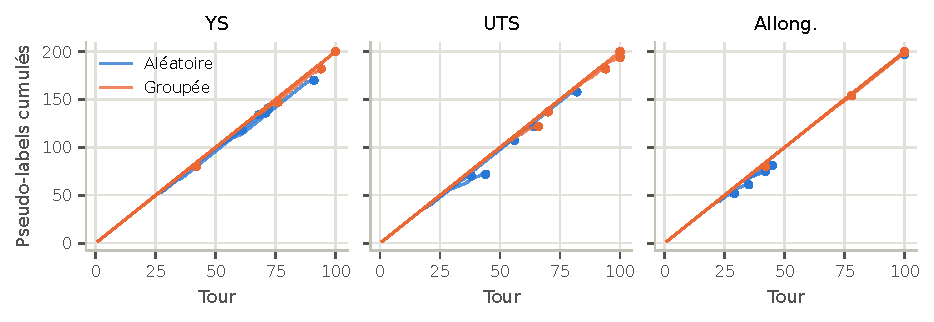
\includegraphics[width=\textwidth]{coreg_iterations}
\caption{Nombre cumulé de pseudo-labels acceptés au fil des tours, pour chacun des
cinq plis externes (un trait par pli ; point : arrêt). La croissance est
quasi linéaire (deux ajouts par tour) jusqu'à l'absence de gain positif ou au
plafond de 100 tours.}
\label{fig:coreg_iter}
\end{figure}

\subsection{Performances}

\begin{figure}[htbp]
\centering
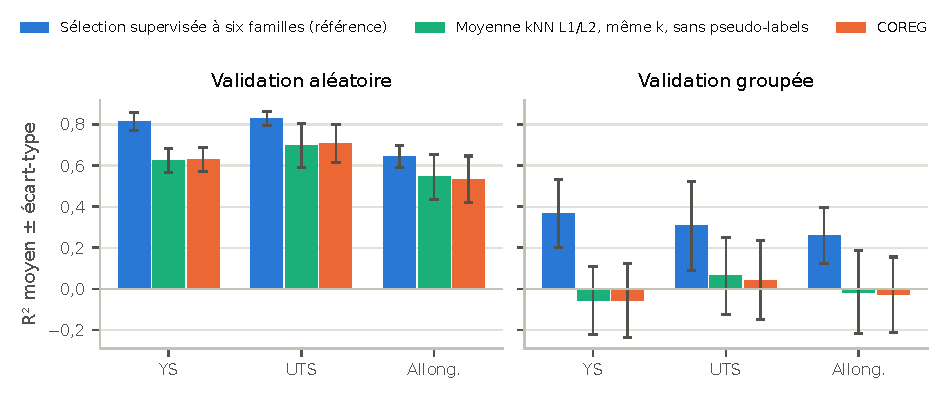
\includegraphics[width=\textwidth]{coreg_comparaison}
\caption{$R^2$ moyen ($\pm$ écart-type) de COREG, de son contrôle apparié sans
pseudo-labels et de la sélection supervisée de référence.}
\label{fig:coreg_comp}
\end{figure}

\begin{table}[htbp]
\centering
\small
\caption{COREG et contrôles : MAE moyenne et $R^2$ moyen sur les cinq plis externes.}
\label{tab:coreg_res}
\setlength{\tabcolsep}{4pt}
\begin{tabular}{@{}l l rr rr rr rr@{}}
\toprule
 & & \multicolumn{2}{c}{COREG} & \multicolumn{2}{c}{$k$NN même $k$} & \multicolumn{2}{c}{$k$NN réglés} & \multicolumn{2}{c}{Supervisé (réf.)} \\
\cmidrule(lr){3-4}\cmidrule(lr){5-6}\cmidrule(lr){7-8}\cmidrule(lr){9-10}
Protocole & Cible & MAE & $R^2$ & MAE & $R^2$ & MAE & $R^2$ & MAE & $R^2$ \\
\midrule
Aléatoire & \YS{} (MPa)   & 37,919 & 0,629 & 38,241 & 0,625 & 38,241 & 0,625 & \meilleur{31,630} & \meilleur{0,755} \\
          & \UTS{} (MPa)  & 33,037 & 0,709 & 33,319 & 0,698 & 33,319 & 0,698 & \meilleur{23,861} & \meilleur{0,836} \\
          & Allong. (pts) & 2,402  & 0,535 & 2,392  & 0,546 & 2,392  & 0,546 & \meilleur{2,054}  & \meilleur{0,660} \\
\midrule
Groupé    & \YS{} (MPa)   & 71,074 & $-0{,}056$ & 70,817 & $-0{,}055$ & 71,717 & $-0{,}080$ & \meilleur{56,757} & \meilleur{0,337} \\
          & \UTS{} (MPa)  & 63,060 & 0,043 & 62,081 & 0,064 & 62,081 & 0,064 & \meilleur{54,344} & \meilleur{0,334} \\
          & Allong. (pts) & 3,904  & $-0{,}028$ & 3,879 & $-0{,}015$ & 3,879 & $-0{,}015$ & \meilleur{3,517} & \meilleur{0,157} \\
\bottomrule
\end{tabular}
\end{table}

\subsection{Gain apparié et robustesse}

Le gain apparié compare COREG et le contrôle au même $k$ sur les mêmes
prédictions hors pli (gain positif = COREG réduit la MAE). L'intervalle est un
bootstrap descriptif par séries (2\,000 tirages).

\begin{table}[htbp]
\centering
\small
\caption{Gain de MAE OOF de COREG par rapport au contrôle apparié (même $k$, sans
pseudo-labels) et par rapport à la sélection supervisée.}
\label{tab:coreg_gain}
\begin{tabular}{@{}l l r l r l@{}}
\toprule
 & & \multicolumn{2}{c}{vs $k$NN même $k$} & \multicolumn{2}{c}{vs supervisé} \\
\cmidrule(lr){3-4}\cmidrule(lr){5-6}
Protocole & Cible & Gain & Intervalle 95\,\% & Gain & Intervalle 95\,\% \\
\midrule
Aléatoire & \YS     & 0,322    & [$-0{,}060$ ; 0,782]   & $-6{,}287$  & [$-11{,}367$ ; $-2{,}070$] \\
          & \UTS    & 0,283    & [$-0{,}154$ ; 0,886]   & $-9{,}175$  & [$-15{,}279$ ; $-3{,}679$] \\
          & Allong. & $-0{,}011$ & [$-0{,}035$ ; 0,013] & $-0{,}349$  & [$-0{,}637$ ; $-0{,}011$] \\
\midrule
Groupé    & \YS     & $-0{,}272$ & [$-1{,}144$ ; 0,523] & $-14{,}245$ & [$-21{,}023$ ; $-6{,}827$] \\
          & \UTS    & $-0{,}920$ & [$-1{,}939$ ; $-0{,}275$] & $-7{,}721$ & [$-18{,}425$ ; 3,331] \\
          & Allong. & $-0{,}024$ & [$-0{,}106$ ; 0,029] & $-0{,}382$  & [$-0{,}780$ ; $-0{,}023$] \\
\bottomrule
\end{tabular}
\end{table}

\paragraph{Lecture des résultats.}
\begin{itemize}
  \item \textbf{Effet propre des pseudo-labels.} En aléatoire, COREG améliore très légèrement la MAE pour \YS{} (0,32\,MPa) et \UTS{} (0,28\,MPa), mais les intervalles couvrent zéro. En groupé, les trois gains sont négatifs, et celui d'\UTS{} est entièrement négatif ([$-1{,}94$ ; $-0{,}28$]\,MPa).
  \item \textbf{Comparaison à la référence.} COREG est moins bon que la sélection supervisée dans \textbf{les six cas}, de 6 à 14\,MPa sur la résistance.
  \item \textbf{Graines.} Avec les graines de base 43 et 44 et le même $k$, les MAE varient de moins de 0,5\,MPa (par exemple \UTS{} aléatoire : 33,04 ; 32,98 ; 33,31) : la conclusion ne dépend pas du tirage des candidats.
\end{itemize}

\subsection{Pourquoi COREG n'apporte-t-il pas de gain ici ?}

Plusieurs explications sont cohérentes avec les mesures, sans qu'aucune ne soit
isolée comme cause unique :
\begin{enumerate}
  \item \textbf{Le régresseur de base est faible hors série.} Les $k$NN sans pseudo-labels ont déjà un $R^2$ proche de zéro en groupé. COREG ne peut que \emph{propager} leurs estimations ; il ne crée pas l'information physique manquante qui permettrait de corriger un décalage entre séries.
  \item \textbf{Le pool apporte peu de diversité.} Après déduplication, seule une fraction du pool est nouvelle, et ces lignes proviennent des mêmes séries que les labels.
  \item \textbf{La confiance est locale.} Le gain $\Delta_u$ mesure la cohérence d'une estimation avec ses voisins étiquetés, pas son exactitude ; les deux $k$NN partagent les mêmes entrées et peuvent renforcer une erreur commune.
  \item \textbf{Le budget de labels est complet.} Le semi-supervisé est surtout utile lorsque les labels sont rares ; ici tous les labels disponibles sont utilisés. Un scénario à 25 ou 50\,\% de labels serait une expérience distincte.
\end{enumerate}

\subsection{Modèles exportés}

Une nouvelle CV5 sur tous les labels (aléatoire graine 1042, ou par groupes) a
choisi $k$ pour les réapprentissages complets : $k = 3$ pour les trois cibles en
aléatoire (82, 44 et 41 pseudo-labels ajoutés), $k = 15$, 5 et 3 en groupé pour
\YS, \UTS{} et l'allongement (200, 186 et 14 pseudo-labels). Au total
\textbf{108 pipelines} sont exportées (90 de plis externes et 18 complètes,
contrôles inclus). Un audit indépendant a recalculé les 180 scores, vérifié
l'isolement des données pour les 576 ajustements et leurs 81\,931 pseudo-labels,
et recalculé explicitement 1\,410 gains.

\begin{aretenir}
COREG a été mis en œuvre selon un protocole inductif rigoureux et comparé à son
exact pendant supervisé. Il \textbf{n'apporte pas de gain significatif} : gains
de l'ordre de 0,3\,MPa non significatifs en aléatoire, gains négatifs en groupé,
et il reste nettement en dessous de la sélection supervisée dans tous les cas.
Les modèles supervisés restent la référence pour cette base.
\end{aretenir}

% =====================================================================
%  10. Analyse comparative, limites et recommandations
% =====================================================================
\clearpage
\section{Analyse comparative et discussion}
\label{sec:discussion}

\subsection{Vue d'ensemble des approches}

Le \cref{tab:recap} rassemble, pour la limite d'élasticité, les principales
approches évaluées au cours du projet. Les autres cibles suivent le même schéma
(\cref{sec:resultats,sec:ssl}).

\begin{table}[htbp]
\centering
\small
\caption{Récapitulatif des approches pour \YS{} : $R^2$ moyen sur cinq plis externes.}
\label{tab:recap}
\begin{tabularx}{\textwidth}{@{}L c c c@{}}
\toprule
Approche & Entrées / imputation & $R^2$ aléatoire & $R^2$ groupé \\
\midrule
Référence médiane de $y$ & -- & $-0{,}031$ & $-0{,}073$ \\
Forêt aléatoire, premier benchmark & 13 / itérative & -- & 0,079 \\
Forêt aléatoire & 13 / médiane & -- & 0,102 \\
Forêt aléatoire & 16 / médiane & 0,765 & 0,390 \\
Sélection conjointe interne (schéma, imputation, famille) & 11--16 / les deux & -- & 0,337 \\
\textbf{Sélection interne de la famille (référence)} & \textbf{16 / médiane} & \textbf{0,755} & \textbf{0,337} \\
$k$NN réglé & 16 / médiane & 0,619 & $-0{,}140$ \\
COREG (semi-supervisé) & 16 / médiane & 0,629 & $-0{,}056$ \\
\bottomrule
\end{tabularx}
\end{table}

Trois enseignements en découlent :
\begin{enumerate}
  \item \textbf{Les entrées comptent davantage que l'algorithme.} Passer de 13 à 16 entrées fait passer le $R^2$ groupé de la forêt de 0,10 à 0,39, alors que changer de famille à entrées fixées modifie beaucoup moins le score.
  \item \textbf{Le protocole change la conclusion.} Toutes les familles apprises perdent entre 0,3 et 0,8 point de $R^2$ entre validation aléatoire et groupée ; les méthodes locales ($k$NN, COREG) deviennent même pires que la constante.
  \item \textbf{Le semi-supervisé n'aide pas ici.} Exploiter les entrées sans label n'apporte pas l'information qui manque pour transférer entre séries.
\end{enumerate}

\subsection{Quelle approche est la plus appropriée ?}

\begin{decision}
L'approche recommandée est la \textbf{procédure supervisée 16 entrées + procédé,
imputation médiane apprise dans le train, avec choix de la famille et des
hyperparamètres par validation interne}. En pratique, cette procédure retient
une \textbf{SVR RBF} ou une \textbf{forêt aléatoire} selon la cible
(\cref{tab:modeles_finaux}) ; la forêt est la plus robuste lorsque la série est
inconnue. COREG est conservé comme expérience semi-supervisée documentée, pas
comme modèle de référence.
\end{decision}

Le niveau de confiance à accorder dépend toutefois de l'usage :
\begin{itemize}
  \item \textbf{Soudure proche d'une série déjà documentée} (même procédé, mêmes familles de composition) : l'erreur typique attendue est d'environ 30\,MPa sur \YS, 25\,MPa sur \UTS{} et 2 points d'allongement --- un ordre de grandeur utile pour pré-sélectionner des recettes avant essais.
  \item \textbf{Soudure d'une nouvelle étude, procédé ou famille d'alliage} : l'erreur double (environ 55\,MPa sur \YS{} et \UTS) et le $R^2$ chute sous 0,35. Le modèle ne remplace pas l'essai mécanique ; il peut au mieux orienter.
  \item \textbf{Énergie Charpy} : les prédictions restent exploratoires tant que les protocoles ne sont pas harmonisés ; elles ne doivent pas servir à une décision de ténacité.
\end{itemize}

\subsection{Limites de l'étude}

\begin{itemize}
  \item \textbf{Sélection rétrospective.} Le passage à 16/médiane a été décidé après observation des scores groupés sur ces mêmes données. Même avec une validation imbriquée ensuite, l'ensemble de la démarche n'a pas été validé sur un jeu indépendant.
  \item \textbf{Groupes imparfaits.} Les séries sont inférées des identifiants : elles peuvent fusionner ou séparer des publications. Elles restent des approximations des vraies unités d'indépendance.
  \item \textbf{Données hétérogènes.} Compositions incomplètes, unités douteuses en quarantaine, protocoles Charpy non harmonisés, précision de transcription inconnue.
  \item \textbf{Entrées omises.} Des éléments exclus pour leur faible couverture (Nb, V, Ti, B, Cu\ldots) peuvent expliquer une partie des décalages entre séries.
  \item \textbf{Incertitude.} Les intervalles rapportés sont descriptifs ; aucune prédiction n'est accompagnée d'un intervalle de prédiction calibré.
  \item \textbf{Semi-supervisé.} Une seule méthode, un seul budget de labels (complet) ; d'autres variantes (régresseurs différents, labels rares) restent à explorer.
\end{itemize}

\subsection{Recommandations}
\label{subsec:recommandations}

L'énoncé demande nos recommandations pour obtenir une bonne qualité de soudure.
Les modèles mettent en évidence des \emph{associations}, pas des causes : nous
séparons donc ce que les données permettent d'affirmer de ce qui demanderait des
essais dédiés.

\paragraph{Ce que l'étude permet de recommander.}
\begin{enumerate}
  \item \textbf{Mesurer et enregistrer la composition complète}, y compris Ni, Cr et Mo : leur ajout réduit l'erreur de 9 à 11\,MPa sur la résistance, alors qu'ils manquent dans plus de la moitié des lignes. Une valeur mesurée vaut mieux qu'une valeur imputée.
  \item \textbf{Documenter le traitement thermique après soudage} (température, durée) : avec la composition, c'est le bloc d'information le plus utilisé par les modèles pour prédire la résistance.
  \item \textbf{Enregistrer les protocoles d'essai}, en particulier pour Charpy : distinguer une énergie mesurée à température imposée d'une température de transition, et conserver des courbes $E(T)$ complètes.
  \item \textbf{Identifier les séries, éprouvettes et publications} dans les bases, afin de pouvoir valider honnêtement le transfert à de nouvelles études.
  \item \textbf{Valider tout modèle sur de nouvelles séries} avec de vraies mesures avant un usage opérationnel, et signaler les soudures hors du domaine du train (procédé inconnu, compositions extrêmes), où l'erreur augmente nettement.
  \item \textbf{Privilégier la diversité des études} plutôt que le nombre de lignes : les courbes d'apprentissage suggèrent que de nouvelles séries sont plus informatives que de nouvelles répétitions.
\end{enumerate}

\paragraph{Ce que l'étude ne permet pas d'affirmer.} Aucun réglage de soudage
\og optimal \fg{}, aucun seuil universel de bonne soudure et aucun effet causal
d'un élément ou d'un paramètre n'est démontré. Les importances indiquent
\emph{quelles} informations le modèle utilise, pas \emph{dans quel sens} modifier
une recette. Pour formuler des recommandations de procédé (composition cible,
apport thermique, PWHT), il faudrait des plans d'expériences contrôlés et
l'expertise de métallurgistes du soudage.

\begin{aretenir}
La procédure supervisée 16/médiane (SVR ou forêt aléatoire selon la cible) est
l'approche la plus appropriée. Elle est fiable pour interpoler dans des séries
connues, nettement moins pour de nouvelles études. Les leviers d'amélioration
sont avant tout la \textbf{qualité et la complétude des données} : composition
complète, PWHT, protocoles d'essai et identification des séries.
\end{aretenir}

% =====================================================================
%  11. Conclusion et perspectives
% =====================================================================
\section{Conclusion et perspectives}
\label{sec:conclusion}

Ce projet a traité la prédiction de la qualité de soudures d'acier comme un
ensemble de \textbf{régressions supervisées} sur des propriétés mécaniques
mesurées. L'analyse exploratoire a révélé une base compilée à partir de séries
expérimentales, avec des absences dépendant du procédé, des valeurs censurées,
des unités douteuses et des protocoles Charpy hétérogènes. Une préparation
entièrement traçable, un prétraitement appris dans chaque pli et une validation
croisée imbriquée selon deux scénarios ont permis une comparaison rigoureuse de
cinq familles supervisées et d'une méthode semi-supervisée.

Les résultats tiennent en trois phrases. \textbf{(1)} Avec 16 entrées et une
imputation médiane, la forêt aléatoire et la SVR RBF prédisent bien les soudures
de séries connues ($R^2$ de 0,66 à 0,84). \textbf{(2)} Le transfert à des séries
absentes reste difficile ($R^2$ de 0,08 à 0,34), principalement à cause de
décalages de niveau entre études que les entrées disponibles n'expliquent pas.
\textbf{(3)} COREG n'améliore pas la référence supervisée, car les entrées sans
label n'apportent pas l'information manquante.

\paragraph{Perspectives.}
\begin{itemize}
  \item \textbf{Validation indépendante} : évaluer la procédure retenue sur de nouvelles séries jamais utilisées pour la concevoir.
  \item \textbf{Enrichir les entrées} : réintégrer Nb, V, Ti, B ou Cu après vérification des unités par source, et tester leur apport par validation groupée.
  \item \textbf{Harmoniser Charpy} : poursuivre l'audit des 21 séries non résolues, séparer courbes $E(T)$ et températures de transition, puis construire une tâche homogène.
  \item \textbf{Quantifier l'incertitude} : intervalles de prédiction (forêts quantiles, prédiction conforme) et détection des entrées hors domaine.
  \item \textbf{Modèles hiérarchiques} : modéliser explicitement un effet aléatoire de série pour séparer variabilité intra- et inter-études.
  \item \textbf{Semi-supervisé} : tester COREG et d'autres méthodes dans un régime à labels rares (25 ou 50\,\%), où leur intérêt théorique est le plus grand.
\end{itemize}

% =====================================================================
%  12. Organisation du projet et diagramme de Gantt
% =====================================================================
\clearpage
\section{Organisation du projet et diagramme de Gantt}
\label{sec:organisation}

\subsection{Méthode de travail}

Le travail a été organisé autour d'un dépôt Git commun (\cref{tab:depot}) :
une branche par tâche, des modèles d'\emph{issue} et de \emph{pull request}, une
spécification vivante (\fichier{specs/spec.md}) consignant chaque décision
scientifique, des rapports intermédiaires datés et une suite de tests ciblés.
Le fichier \fichier{specs/time\_log.csv} est prévu pour enregistrer le temps
passé par membre et par séance.

\subsection{Chronologie et diagramme de Gantt}

La \cref{fig:gantt} retrace les grandes phases du projet. Les dates proviennent
de l'historique Git et des dates portées par les rapports intermédiaires : elles
indiquent \emph{quand} chaque livrable a été produit ou versionné, pas la durée
de travail effective.

\begin{figure}[htbp]
\centering
\begin{ganttchart}[
    hgrid, vgrid={*1{draw=black!12}},
    time slot format=isodate,
    x unit=0.98cm, y unit chart=0.58cm, y unit title=0.55cm,
    title height=1,
    title label font=\scriptsize\bfseries,
    bar label font=\scriptsize,
    group label font=\scriptsize\bfseries,
    milestone label font=\scriptsize\itshape,
    bar/.append style={fill=csbordeaux!70, draw=csbordeaux},
    bar height=0.55,
    group/.append style={fill=csgris, draw=csgris},
    group height=0.25,
    milestone/.append style={fill=orangeviz, draw=orangeviz},
    bar label node/.append style={align=right},
  ]{2026-10-02}{2026-10-11}
  \gantttitle{Octobre 2026}{10} \\
  \gantttitlecalendar{day} \\
  \ganttgroup{Cadrage et données}{2026-10-02}{2026-10-07} \\
  \ganttbar{Dépôt, énoncé, téléchargement}{2026-10-02}{2026-10-03} \\
  \ganttbar{Audit exploratoire (EDA)}{2026-10-03}{2026-10-07} \\
  \ganttbar{Essais de prétraitement, ACP}{2026-10-05}{2026-10-05} \\
  \ganttgroup{Préparation et protocole}{2026-10-08}{2026-10-09} \\
  \ganttbar{Audit et migration (notebook 02)}{2026-10-08}{2026-10-08} \\
  \ganttbar{Cibles et plan d'expériences}{2026-10-09}{2026-10-09} \\
  \ganttgroup{Modélisation et analyse}{2026-10-10}{2026-10-10} \\
  \ganttbar{Supervisé et diagnostics (03, 04)}{2026-10-10}{2026-10-10} \\
  \ganttbar{CV aléatoire, exports (05, 06)}{2026-10-10}{2026-10-10} \\
  \ganttbar{COREG (07)}{2026-10-10}{2026-10-10} \\
  \ganttgroup{Rédaction}{2026-10-10}{2026-10-11} \\
  \ganttbar{Synthèses et rapports}{2026-10-10}{2026-10-11} \\
  \ganttmilestone{Rendu final (date à compléter)}{2026-10-11}
\end{ganttchart}
\caption{Diagramme de Gantt des phases du projet, d'après l'historique Git et les
dates des rapports intermédiaires. Les responsables et les heures réelles sont
à renseigner dans le \cref{tab:taches} ; la date de rendu est indicative.}
\label{fig:gantt}
\end{figure}

\subsection{Répartition des tâches et temps passé}

L'énoncé demande d'indiquer, pour chaque tâche, le temps qu'elle a pris et le
membre de l'équipe qui s'en est chargé. Ces informations ne sont pas déductibles
des fichiers du dépôt (le journal de temps est vide) : elles sont laissées
\emph{à compléter par l'équipe}, sans être inventées. Les durées de calcul des
notebooks (quelques minutes chacun) ne sont pas des durées de travail humain.

\begin{table}[htbp]
\centering
\small
\caption{Répartition des tâches. Colonnes \og Membre(s) \fg{} et \og Heures \fg{} à
compléter par l'équipe à partir de \fichier{specs/time\_log.csv}.}
\label{tab:taches}
\begin{tabularx}{\textwidth}{@{}L l l l@{}}
\toprule
Tâche & Livrables & Membre(s) & Heures \\
\midrule
Cadrage, dépôt, téléchargement des données & \fichier{scripts/}, \fichier{specs/} & \acompleter{} & \acompleter{} \\
Analyse exploratoire et audit des mesures & notebook 01, rapport 01 & \acompleter{} & \acompleter{} \\
Prétraitement, groupes, cohorte, plis & notebook 02, rapports 02--08 & \acompleter{} & \acompleter{} \\
Plan d'expériences, choix des cibles & rapport 09, \fichier{spec.md} & \acompleter{} & \acompleter{} \\
Entraînement supervisé & notebooks 03, 05, 06 & \acompleter{} & \acompleter{} \\
Diagnostics et explicabilité & notebook 04, rapport 11 & \acompleter{} & \acompleter{} \\
Bibliographie et COREG & notebook 07, rapport 14 & \acompleter{} & \acompleter{} \\
Tests et reproductibilité & \fichier{tests/}, manifestes & \acompleter{} & \acompleter{} \\
Rédaction et relecture croisée & rapports 15, 16, présent rapport & \acompleter{} & \acompleter{} \\
\midrule
\textbf{Total} & & & \acompleter{} \\
\bottomrule
\end{tabularx}
\end{table}

\begin{aretenir}
Le projet s'est déroulé du 2 au 10 octobre 2026 pour sa partie technique, en
quatre phases : cadrage et données, préparation et protocole, modélisation et
analyse, rédaction. La répartition des tâches et les heures réelles restent à
renseigner par l'équipe.
\end{aretenir}


% ---------- Bibliographie -------------------------------------------
\clearpage
\phantomsection
\addcontentsline{toc}{section}{Références bibliographiques}
\bibliographystyle{unsrtnat}
\renewcommand{\bibname}{Références bibliographiques}
\renewcommand{\refname}{Références bibliographiques}
\bibliography{references}

% ---------- Annexes -------------------------------------------------
\clearpage
\appendix
\renewcommand{\thesection}{\Alph{section}}
% =====================================================================
%  Annexe A — Dictionnaire des variables
% =====================================================================
\section{Dictionnaire des variables}
\label{annexe:variables}

Positions et unités d'après la documentation de la base~\cite{cool_welddb} ; noms
utilisés dans les notebooks. Colonne \og Usage \fg{} : E11/E13/E16 = entrée des
schémas 11, 13 ou 16 (\cref{tab:schemas}) ; C = cible ; X = non utilisée.

{\footnotesize
\begin{longtable}{@{}r l >{\raggedright\arraybackslash}p{4.7cm} >{\raggedright\arraybackslash}p{2.6cm} >{\raggedright\arraybackslash}p{2.4cm}@{}}
\caption{Les 44 champs de la Cambridge Weld Database.}\label{tab:dictionnaire}\\
\toprule
Pos. & Nom (notebooks) & Signification & Unité & Usage \\
\midrule
\endfirsthead
\toprule
Pos. & Nom (notebooks) & Signification & Unité & Usage \\
\midrule
\endhead
\bottomrule
\endfoot
1  & \texttt{C}  & Carbone   & \% massique & E11 \\
2  & \texttt{Si} & Silicium  & \% massique & E11 \\
3  & \texttt{Mn} & Manganèse & \% massique & E11 \\
4  & \texttt{S}  & Soufre    & \% massique & E11 \\
5  & \texttt{P}  & Phosphore & \% massique & E11 \\
6  & \texttt{Ni} & Nickel    & \% massique & E16 \\
7  & \texttt{Cr} & Chrome    & \% massique & E16 \\
8  & \texttt{Mo} & Molybdène & \% massique & E16 \\
9  & \texttt{V}  & Vanadium  & \% massique & X \\
10 & \texttt{Cu} & Cuivre    & \% massique & X \\
11 & \texttt{Co} & Cobalt    & \% massique & X \\
12 & \texttt{W}  & Tungstène & \% massique & X \\
13 & \texttt{O\_ppm}  & Oxygène   & ppm & E13 \\
14 & \texttt{Ti\_ppm} & Titane    & ppm (unité à revoir) & X \\
15 & \texttt{N\_ppm}  & Azote     & ppm & E13 \\
16 & \texttt{Al\_ppm} & Aluminium & ppm (unité à revoir) & X \\
17 & \texttt{B\_ppm}  & Bore      & ppm & X \\
18 & \texttt{Nb\_ppm} & Niobium   & ppm & X \\
19 & \texttt{Sn\_ppm} & Étain     & ppm (unité à revoir) & X \\
20 & \texttt{As\_ppm} & Arsenic   & ppm (unité à revoir) & X \\
21 & \texttt{Sb\_ppm} & Antimoine & ppm (unité à revoir) & X \\
22 & \texttt{current\_A} & Courant de soudage & A & E11 \\
23 & \texttt{voltage\_V} & Tension            & V & E11 \\
24 & \texttt{ac\_dc}     & Type de courant (AC/DC) & catégoriel & X \\
25 & \texttt{polarity}  & Polarité de l'électrode & catégoriel & X \\
26 & \texttt{heat\_input\_kJmm} & Apport thermique & kJ/mm & E11 \\
27 & \texttt{interpass\_C} & Température entre passes & °C & E11 \\
28 & \texttt{weld\_type} & Procédé de soudage & catégoriel & tous schémas \\
29 & \texttt{pwht\_temp\_C} & Température du traitement après soudage & °C & E11 \\
30 & \texttt{pwht\_time\_h} & Durée du traitement après soudage & h & E11 \\
31 & \texttt{yield\_strength} & Limite d'élasticité & MPa & C \\
32 & \texttt{uts} & Résistance maximale à la traction & MPa & C \\
33 & \texttt{elongation} & Allongement & \% & C \\
34 & \texttt{reduction\_area} & Réduction de section & \% & X (complémentaire) \\
35 & \texttt{charpy\_temp\_C} & Température d'essai Charpy & °C & entrée Charpy \\
36 & \texttt{charpy\_J} & Énergie Charpy & J & C (exploratoire) \\
37 & \texttt{hardness} & Dureté (protocole Vickers séparé) & kg/mm$^2$ & X \\
38 & \texttt{fatt50} & Température de transition à 50\,\% de rupture ductile & non documentée & X \\
39 & \texttt{prim\_ferrite} & Ferrite primaire & \% & X \\
40 & \texttt{ferrite\_2nd\_phase} & Ferrite à seconde phase & \% & X \\
41 & \texttt{acicular\_ferrite} & Ferrite aciculaire & \% & X \\
42 & \texttt{martensite} & Martensite & \% & X \\
43 & \texttt{ferrite\_carbide} & Agrégat ferrite-carbure & \% & X \\
44 & \texttt{weld\_id} & Identifiant de la soudure et de sa source & texte & X (sert aux groupes) \\
\end{longtable}
}

Dans la table maître, le procédé est stocké en \texttt{weld\_type\_raw} (brut)
et \texttt{weld\_process} (synonymes regroupés) ; la dureté en
\texttt{hardness\_value} et \texttt{hardness\_protocol}. Les colonnes
\texttt{n\_unavail\_A1\_13}, \texttt{in\_strict13} et \texttt{has\_<cible>}
définissent la cohorte et l'éligibilité de chaque cible.

% =====================================================================
%  Annexe B — Reproductibilité
% =====================================================================
\section{Reproductibilité}
\label{annexe:reproductibilite}

\subsection{Environnement}

Les expériences ont été exécutées avec Python 3.14.8, scikit-learn 1.9.1,
NumPy 2.5.3, pandas 3.0.6, joblib 1.6.0 et cloudpickle 3.1.2 ; les versions
exactes sont enregistrées dans chaque manifeste d'expérience. Le fichier brut
\fichier{welddb.data} a pour empreinte SHA-256 :

\begin{center}
\footnotesize\texttt{eb46df81a454c8e549187d87c67a6e72b88676f760e8688a782c832737676ac1}
\end{center}

\subsection{Commandes}

Depuis la racine du dépôt :
\begin{verbatim}
python -m venv .venv && source .venv/bin/activate
python -m pip install -r requirements.txt
python scripts/download_data.py           # archive vérifiée par SHA-256
python -m jupyterlab                      # exécuter 01 -> 07 de haut en bas
python -m unittest discover -s tests -v   # 37 tests ciblés hors ligne
python rapport_latex/scripts/generer_figures.py
cd rapport_latex && latexmk -pdf main.tex
\end{verbatim}

\subsection{Notebooks, durées et exports}

\begin{table}[htbp]
\centering
\small
\caption{Notebooks, durée de calcul rapportée dans les rapports d'exécution et exports produits (ignorés par Git).}
\label{tab:notebooks}
\begin{tabularx}{\textwidth}{@{}l L l@{}}
\toprule
Notebook & Rôle et exports & Durée \\
\midrule
01\_eda & Statuts, distributions, ACP descriptive ; aucun export d'entraînement & non mesurée \\
02\_data\_preparation & Table maître, provenance, alias, groupes, plis, cellules en quarantaine, manifeste (\fichier{data/processed/modeling/}) & non mesurée \\
03\_modeling & Benchmark 13/itérative groupé : 100 évaluations, 2\,440 ajustements (\fichier{salh\_supervised\_v1/}) & $\approx 6$\,min \\
04\_diagnostics & Erreurs par série, sensibilités 11/13/16, permutations, audit Charpy (\fichier{salh\_diagnostics\_v1/}) & non mesurée \\
05\_random\_kfold & CV aléatoire 16/médiane, 40 pipelines (\fichier{salh\_random\_kfold\_v1/}) & $\approx 7$\,min \\
06\_grouped\_exports & CV groupée 16/médiane, 40 pipelines (\fichier{salh\_group\_kfold\_v1/}) & $\approx 2$\,min \\
07\_coreg & COREG, contrôles, 108 pipelines (\fichier{salh\_coreg\_v1/}) & $\approx 10$\,min \\
\bottomrule
\end{tabularx}
\end{table}

Les modèles sont sérialisés sous \fichier{models/} avec un fichier JSON compagnon
(entrées, unités, identifiants du train, paramètres, graines, versions, SHA-256) :
40 pipelines pour la CV aléatoire, 40 pour la CV groupée et 108 pour COREG, soit
\textbf{188 pipelines}. Chaque dossier possède un index \fichier{selected\_models.json}.
Les modèles réentraînés sur tous les labels servent à l'inférence uniquement.

\subsection{Contrôles automatiques}

La suite de 37 tests hors ligne vérifie notamment : l'intégrité des archives,
la classification des statuts de mesure, les doublons et les groupes, l'apprentissage
des statistiques dans le seul train, la préservation des valeurs observées, les
erreurs explicites (PWHT, non-convergence), l'étanchéité des recherches imbriquées,
l'échelle des cibles de la SVR, les frontières des pools inductifs, et, pour COREG,
l'égalité du gain local calculé avec un réapprentissage explicite. Des audits
indépendants recalculent les métriques à partir des prédictions exportées et
rechargent tous les modèles dans un processus Python neuf.

\subsection{Figures de ce rapport}

Les figures du dossier \ident{rapport_latex/figures/} sont produites par le script
\ident{rapport_latex/scripts/generer_figures.py}, qui relit le fichier brut et
les exports des notebooks sans réentraîner aucun modèle. Le script affiche les
valeurs clés recalculées (effectifs, variance expliquée par l'ACP) afin de vérifier
leur cohérence avec le texte.

% =====================================================================
%  Annexe C — Tableaux complémentaires
% =====================================================================
\section{Tableaux complémentaires}
\label{annexe:tableaux}

\subsection{Familles supervisées, configuration 16/médiane}

\begin{table}[htbp]
\centering
\small
\caption{Validation aléatoire : chaque famille réglée en interne (moyenne $\pm$
écart-type sur 5 plis ; RMSE moyenne).}
\label{tab:annexe_aleatoire}
\begin{tabular}{@{}l l r r r@{}}
\toprule
Cible & Modèle & MAE & RMSE & $R^2$ \\
\midrule
\YS{} (MPa) & Médiane de $y$  & 70,032 $\pm$ 4,087 & 92,774 & $-0{,}031 \pm 0{,}040$ \\
            & Ridge           & 54,047 $\pm$ 3,440 & 70,005 & $0{,}412 \pm 0{,}053$ \\
            & SVR RBF         & 31,747 $\pm$ 3,900 & 45,403 & $0{,}754 \pm 0{,}046$ \\
            & Forêt aléatoire & 31,242 $\pm$ 4,038 & 44,172 & $0{,}765 \pm 0{,}064$ \\
            & $k$NN           & 38,144 $\pm$ 2,497 & 56,273 & $0{,}619 \pm 0{,}059$ \\
\midrule
\UTS{} (MPa) & Médiane de $y$ & 68,879 $\pm$ 4,438 & 91,419 & $-0{,}050 \pm 0{,}019$ \\
             & Ridge          & 44,319 $\pm$ 3,535 & 60,137 & $0{,}538 \pm 0{,}118$ \\
             & SVR RBF        & 23,861 $\pm$ 0,906 & 35,989 & $0{,}836 \pm 0{,}027$ \\
             & Forêt aléatoire & 26,906 $\pm$ 1,907 & 39,165 & $0{,}805 \pm 0{,}045$ \\
             & $k$NN          & 33,452 $\pm$ 4,870 & 48,626 & $0{,}697 \pm 0{,}098$ \\
\midrule
Allong. (pts) & Médiane de $y$ & 4,019 $\pm$ 0,149 & 4,903 & $-0{,}015 \pm 0{,}019$ \\
              & Ridge          & 3,011 $\pm$ 0,152 & 3,923 & $0{,}345 \pm 0{,}119$ \\
              & SVR RBF        & 2,268 $\pm$ 0,198 & 3,227 & $0{,}556 \pm 0{,}094$ \\
              & Forêt aléatoire & 2,054 $\pm$ 0,239 & 2,835 & $0{,}660 \pm 0{,}058$ \\
              & $k$NN          & 2,423 $\pm$ 0,260 & 3,305 & $0{,}530 \pm 0{,}117$ \\
\midrule
\charpy{} (J) & Médiane de $y$ & 36,756 $\pm$ 2,813 & 51,989 & $-0{,}069 \pm 0{,}037$ \\
              & Ridge          & 26,913 $\pm$ 0,587 & 34,170 & $0{,}529 \pm 0{,}113$ \\
              & SVR RBF        & 17,393 $\pm$ 0,988 & 25,068 & $0{,}749 \pm 0{,}043$ \\
              & Forêt aléatoire & 16,099 $\pm$ 1,027 & 22,636 & $0{,}795 \pm 0{,}035$ \\
              & $k$NN          & 19,253 $\pm$ 1,518 & 29,586 & $0{,}651 \pm 0{,}055$ \\
\bottomrule
\end{tabular}
\end{table}

\begin{table}[htbp]
\centering
\small
\caption{Validation groupée : chaque famille réglée en interne (moyenne $\pm$
écart-type sur 5 plis ; RMSE moyenne).}
\label{tab:annexe_groupee}
\begin{tabular}{@{}l l r r r@{}}
\toprule
Cible & Modèle & MAE & RMSE & $R^2$ \\
\midrule
\YS{} (MPa) & Médiane de $y$  & 70,449 $\pm$ 10,682 & 92,501 & $-0{,}073 \pm 0{,}052$ \\
            & Ridge           & 69,387 $\pm$ 6,953  & 88,202 & $-0{,}025 \pm 0{,}362$ \\
            & SVR RBF         & 59,350 $\pm$ 9,755  & 76,275 & $0{,}264 \pm 0{,}144$ \\
            & Forêt aléatoire & 54,139 $\pm$ 10,658 & 69,570 & $0{,}390 \pm 0{,}132$ \\
            & $k$NN           & 73,496 $\pm$ 9,189  & 94,956 & $-0{,}140 \pm 0{,}151$ \\
\midrule
\UTS{} (MPa) & Médiane de $y$ & 72,664 $\pm$ 15,237 & 93,729 & $-0{,}180 \pm 0{,}114$ \\
             & Ridge          & 61,898 $\pm$ 13,272 & 77,232 & $0{,}179 \pm 0{,}152$ \\
             & SVR RBF        & 52,861 $\pm$ 11,679 & 70,542 & $0{,}316 \pm 0{,}145$ \\
             & Forêt aléatoire & 48,905 $\pm$ 7,269 & 65,236 & $0{,}394 \pm 0{,}160$ \\
             & $k$NN          & 68,538 $\pm$ 14,821 & 90,258 & $-0{,}115 \pm 0{,}121$ \\
\midrule
Allong. (pts) & Médiane de $y$ & 4,086 $\pm$ 0,309 & 4,962 & $-0{,}062 \pm 0{,}047$ \\
              & Ridge          & 3,658 $\pm$ 0,362 & 4,735 & $0{,}016 \pm 0{,}229$ \\
              & SVR RBF        & 3,670 $\pm$ 0,345 & 4,534 & $0{,}106 \pm 0{,}167$ \\
              & Forêt aléatoire & 3,339 $\pm$ 0,342 & 4,218 & $0{,}226 \pm 0{,}146$ \\
              & $k$NN          & 3,983 $\pm$ 0,328 & 4,908 & $-0{,}060 \pm 0{,}223$ \\
\midrule
\charpy{} (J) & Médiane de $y$ & 36,035 $\pm$ 16,909 & 50,603 & $-0{,}149 \pm 0{,}251$ \\
              & Ridge          & 34,752 $\pm$ 10,268 & 45,433 & $0{,}069 \pm 0{,}213$ \\
              & SVR RBF        & 35,963 $\pm$ 8,404  & 44,879 & $0{,}091 \pm 0{,}206$ \\
              & Forêt aléatoire & 33,033 $\pm$ 10,974 & 43,560 & $0{,}138 \pm 0{,}209$ \\
              & $k$NN          & 35,725 $\pm$ 12,222 & 48,624 & $-0{,}099 \pm 0{,}354$ \\
\bottomrule
\end{tabular}
\end{table}

\subsection{COREG : dispersion et scores OOF}

\begin{table}[htbp]
\centering
\small
\caption{COREG : moyenne $\pm$ écart-type sur les plis et scores OOF réunis.}
\label{tab:annexe_coreg}
\begin{tabular}{@{}l l r r r r@{}}
\toprule
Protocole & Cible & MAE moyenne & $R^2$ moyen & MAE OOF & $R^2$ OOF \\
\midrule
Aléatoire & \YS{} (MPa)   & 37,919 $\pm$ 3,151  & $0{,}629 \pm 0{,}060$ & 37,913 & 0,631 \\
          & \UTS{} (MPa)  & 33,037 $\pm$ 4,905  & $0{,}709 \pm 0{,}093$ & 33,038 & 0,707 \\
          & Allong. (pts) & 2,402 $\pm$ 0,258   & $0{,}535 \pm 0{,}112$ & 2,403  & 0,538 \\
Groupé    & \YS{} (MPa)   & 71,074 $\pm$ 14,263 & $-0{,}056 \pm 0{,}181$ & 71,780 & $-0{,}051$ \\
          & \UTS{} (MPa)  & 63,060 $\pm$ 15,175 & $0{,}043 \pm 0{,}193$ & 61,470 & 0,146 \\
          & Allong. (pts) & 3,904 $\pm$ 0,311   & $-0{,}028 \pm 0{,}183$ & 3,883  & 0,018 \\
\bottomrule
\end{tabular}
\end{table}

\begin{table}[htbp]
\centering
\small
\caption{Sensibilité de COREG à la graine de tirage des candidats ($k$ fixé par la
sélection interne du calcul principal) : MAE moyenne et $R^2$ moyen.}
\label{tab:annexe_graines}
\begin{tabular}{@{}l l rr rr rr@{}}
\toprule
 & & \multicolumn{2}{c}{Graine 42} & \multicolumn{2}{c}{Graine 43} & \multicolumn{2}{c}{Graine 44} \\
\cmidrule(lr){3-4}\cmidrule(lr){5-6}\cmidrule(lr){7-8}
Protocole & Cible & MAE & $R^2$ & MAE & $R^2$ & MAE & $R^2$ \\
\midrule
Aléatoire & \YS     & 37,919 & 0,629 & 37,990 & 0,628 & 38,203 & 0,627 \\
          & \UTS    & 33,037 & 0,709 & 32,976 & 0,709 & 33,314 & 0,703 \\
          & Allong. & 2,402  & 0,535 & 2,397  & 0,535 & 2,396  & 0,538 \\
Groupé    & \YS     & 71,074 & $-0{,}056$ & 70,873 & $-0{,}054$ & 70,868 & $-0{,}051$ \\
          & \UTS    & 63,060 & 0,043 & 62,707 & 0,049 & 63,083 & 0,040 \\
          & Allong. & 3,904  & $-0{,}028$ & 3,887 & $-0{,}018$ & 3,888 & $-0{,}023$ \\
\bottomrule
\end{tabular}
\end{table}

\subsection{Reconstruction de valeurs Ni/Cr/Mo masquées}

\begin{table}[htbp]
\centering
\small
\caption{Erreur absolue moyenne (\% massique) de reconstruction de 20\,\% des
valeurs observées de Ni, Cr et Mo masquées en validation, imputeur ajusté sur le
train ; mêmes cellules pour les deux méthodes.}
\label{tab:annexe_masquage}
\begin{tabular}{@{}l l rr rr rr@{}}
\toprule
 & & \multicolumn{2}{c}{Ni} & \multicolumn{2}{c}{Cr} & \multicolumn{2}{c}{Mo} \\
\cmidrule(lr){3-4}\cmidrule(lr){5-6}\cmidrule(lr){7-8}
Contexte & Imputation & $n$ & MAE & $n$ & MAE & $n$ & MAE \\
\midrule
\YS     & médiane   & 71 & 0,388 & 71 & 1,612 & 70 & 0,388 \\
        & itérative & 71 & 0,419 & 71 & 1,419 & 70 & 0,313 \\
\UTS    & médiane   & 45 & 0,439 & 52 & 1,556 & 43 & 0,370 \\
        & itérative & 45 & 0,537 & 52 & 1,705 & 43 & 0,399 \\
Allong. & médiane   & 58 & 0,325 & 64 & 1,098 & 58 & 0,407 \\
        & itérative & 58 & 0,723 & 64 & 1,945 & 58 & 0,362 \\
Charpy  & médiane   & 33 & 0,782 & 40 & 1,504 & 30 & 0,696 \\
        & itérative & 33 & 1,035 & 40 & 4,792 & 30 & 1,060 \\
\bottomrule
\end{tabular}
\end{table}

% =====================================================================
%  Annexe D — Glossaire
% =====================================================================
\section{Glossaire}
\label{annexe:glossaire}

\begin{description}[leftmargin=0pt,itemsep=0.35em,font=\bfseries\color{csbordeaux}]
  \item[Apport thermique] Énergie électrique fournie par unité de longueur de soudure (kJ/mm) ; dépend du courant, de la tension et de la vitesse de soudage.
  \item[Biais d'une série] Erreur moyenne (prédit $-$ observé) des observations d'une même série ; un biais non nul signifie que le modèle se trompe de niveau pour toute la série.
  \item[Bootstrap par groupes] Rééchantillonnage avec remise des séries (et non des lignes) pour estimer la variabilité d'un indicateur lorsque les lignes d'une série sont dépendantes.
  \item[Censure] Valeur rapportée seulement comme inférieure à une limite de détection (\texttt{<L}).
  \item[Charpy (essai)] Essai de choc sur éprouvette entaillée mesurant l'énergie absorbée à la rupture (J) à une température donnée ; renseigne sur la ténacité.
  \item[Cohorte] Population de lignes retenue pour la modélisation (ici : au plus deux entrées manquantes sur 13, sans doublon).
  \item[COREG] Méthode de co-apprentissage pour la régression : deux $k$NN s'échangent des pseudo-labels choisis par réduction locale d'erreur.
  \item[Fuite d'information] Utilisation, pendant l'apprentissage, d'une information issue des données de validation ; elle rend les scores optimistes.
  \item[GroupKFold] Validation croisée qui place toutes les observations d'un même groupe dans le même pli.
  \item[Imputation] Remplacement d'une entrée manquante par une valeur estimée (médiane, régression itérative\ldots) ; ce n'est pas une mesure.
  \item[Inductif / transductif] Un protocole semi-supervisé est inductif s'il n'utilise jamais les entrées de validation pendant l'apprentissage, transductif s'il les exploite sans leurs labels.
  \item[MAE, RMSE, $R^2$] Erreur absolue moyenne, racine de l'erreur quadratique moyenne, coefficient de détermination (\cref{subsec:metriques}).
  \item[OOF (\emph{out-of-fold})] Prédiction faite pour une observation par le modèle du pli où elle était en validation ; l'ensemble des OOF couvre chaque label une fois.
  \item[Pipeline] Enchaînement d'étapes de prétraitement et d'un estimateur, ajusté en bloc sur le train puis appliqué tel quel à de nouvelles données.
  \item[Pli (\emph{fold})] Partie des données tenue à l'écart pour l'évaluation pendant une itération de validation croisée.
  \item[Pool non étiqueté] Lignes qui ne renseignent pas la cible, utilisables par une méthode semi-supervisée.
  \item[Pseudo-label] Valeur de cible estimée par un modèle et ajoutée comme label ; ce n'est pas une mesure.
  \item[PWHT] Traitement thermique après soudage (\emph{post-weld heat treatment}), caractérisé par une température et une durée.
  \item[Série inférée] Groupe d'observations issues d'une même étude, déduit des identifiants ; utilisé pour la validation groupée.
  \item[Standardisation] Transformation $z = (x - \mu)/\sigma$ qui met les variables à la même échelle.
  \item[Validation croisée imbriquée] Validation à deux niveaux : la boucle interne règle le modèle, la boucle externe l'évalue sur des données jamais utilisées pour le régler.
  \item[\YS, \UTS] Limite d'élasticité et résistance maximale à la traction (MPa).
\end{description}


\end{document}
